% Yu-Ting Lu 24/7/2011 (Swansea)

\documentclass[11pt]{report}

\usepackage{hyperref}
\usepackage{a4}
\usepackage{subfigure}
\usepackage{sudoku}
\usepackage{amsmath}
\usepackage{colortbl}
\usepackage{multirow}
\usepackage[normalem]{ulem}
\usepackage{tikz}
\usetikzlibrary{shapes,arrows,calc}


\setlength\sudokusize{8cm}
\newcommand{\cell}[9]{%
\scriptsize
\setlength{\tabcolsep}{1pt}
\renewcommand{\arraystretch}{0.5}
\hspace{-0.6em}
\begin{tabular}{ccc}
#1 & #2 & #3\\
#4 & #5 & #6\\
#7 & #8 & #9
\end{tabular}
}

\newcommand{\set}[1]{\{ #1 \}}


\begin{document}

\begin{titlepage}
\centering

\includegraphics[width=0.6\textwidth]{./logo.jpg}\\ \vspace{50pt}
\Large \textbf{Sudoku Patterns}\\ \vspace{20pt}
Project Dissertation submitted to Swansea University\\ \vspace{6pt}
in Partial Fulfilment for the Degree of Master of Science  in\\ \vspace{12pt}
 \textbf{Computing and Software Technology}\\ \vspace{30pt}
\large \textbf{Submitted by:}\\ \vspace{6pt}
Yu-Ting Lu\\ \vspace{6pt}
461467 \\ \vspace{30pt}
\textbf{Under the Supervision of:}\\ \vspace{6pt}
Dr. Oliver Kullman\\ \vspace{30pt}
\textbf{Project Conducted at:}\\ \vspace{6pt}
Department of computer Science, Swansea University\\ \vspace{6pt}
Singleton Park, Swanse SA2 8PP, Wales, UK\\ \vspace{6pt}
September, 2011\\ \vspace{12pt}
\end{titlepage}


\begin{abstract}
Many rules for solving a Sudoku instance have been introduced for a standard instance in a row-column view. In this report, we have ``square'' and original elements (row, column, block, number) involved to get three additional extended view generated from the standard one in different dimensions instead of having a Sudoku instance only in a standard row-column view. Three other views are, row-number view, column-number view, and block-number view.

During finding a solution by matching all the rules with the annotated instance, have four different views for an annotated instance could make it use the simple rule as far as possible. It could cut down the time consuming on the rule matching, and also carry out a solution for the annotated instance as soon as it can.
\end{abstract}


\textbf{DECLARATION}\\
This work has not previously been accepted in substance for any degree and is not being concurrently submitted in candidature for any degree.\\
\textbf{STATEMENT 1}\\
This dissertation is the result of my own independent work/investigation, except where otherwise stated. Other sources are acknowledged by giving explicit references. A bibliography is appended.\\
\textbf{STATEMENT 2}\\
I hereby give consent for my dissertation, if accepted, to be available for photocopying and for inter-library loan, and for the title and summary to be made available to outside organisations.


\tableofcontents



\chapter{Introduction}
\label{cha:Introduction}


Sudoku is a puzzle which is popularised into the world for ages. And there are amount of people spend times on either hard puzzle generated, or looking for the best techniques to improve the efficiency on solving difficult puzzle.
When the puzzle difficulty becomes harder and harder, then more advanced techniques will be required to be used together or in order to cope the puzzle. Surely, as the difficulties level goes up, the cost of time raise up even thought the suitable technique is given to help. Consequently, in this report, the first chapter is going to know the background of Sudoku and what is Sudoku, and the secondly understand discussed after understanding how these special techniques applied on eliminating impossibilities in puzzle solving. Afterwards, the efficiency of the special technique for solving Sudoku will be the final topic to discuss about in the end.
In this dissertation, the goal to achieve is to experience the time of applying special techniques on solving Sudoku puzzles. In addition, to find out the most efficient way to apply the combination of more than techniques and how many puzzles could it achieve to solve.


\section{What is Sudoku?}
\label{sec:whatissudoku}

Sudoku uses an $N \times N$ matrix, where $N = n \cdot n$, and for standard Sudoku we have $n = 3$, thus $N = 9$. Each entry (``cell'') contains a number in $\{1, \dots, N\}$, or it might be empty, that is, to be filled out. A completed Sudoku puzzle must fulfil the following additional requirements:
\begin{enumerate}
\item In every row and in every column every number occurs only (exactly) once.
\item The same is true for the ``blocks'':
\begin{enumerate}
\item The whole matrix is sub-divided into $N$ blocks.
\item Each block is an $n \times n$ matrix.
\end{enumerate}
Now in each block every number has also to occur (exactly) once.
\end{enumerate}
For ``classical Sudoku'' puzzles we have the following additional rules:
\begin{enumerate}
\item A Sudoku puzzle must have at least one solution (no unsolvable puzzles are normally considered).
\item And in fact, a Sudoku puzzle must have a unique solution (no multiple solutions are normally allowed).
\end{enumerate}
An example is given with Figure \ref{sudokuEx}, while for the solution see Figure \ref{fig:solutionsudokuEx}.

\begin{figure}[htbp]
\begin{sudoku}
 |1| | |2| | | | |4|.
 | |9| |5| |3|6|7| |.
 | |4| | |7| | | | |.
 | |1| | | | | |5|9|.
 | | |2| | | |3| | |.
 |9|7| | | || |2| |.
 | | | | |1| | |6| |.
 | |8|5|3| |9| |1| |.
 |4| | | | |6| | |5|.
\end{sudoku}
\caption{An example for a Sudoku problem}
\label{sudokuEx}
\end{figure}

\begin{figure}[htbp]
\begin{sudoku}
  |1|5|7|2|6|8|9|3|4|.
  |2|9|8|5|4|3|6|7|1|.
  |3|4|6|9|7|1|5|8|2|.
  |8|1|4|6|3|2|7|5|9|.
  |5|6|2|1|9|7|3|4|8|.
  |9|7|3|8|5|4|1|2|6|.
  |7|2|9|4|1|5|8|6|3|.
  |6|8|5|3|2|9|4|1|7|.
  |4|3|1|7|8|6|2|9|5|.
\end{sudoku}
\caption{The solution for the Sudoku problem given in Figure \ref{sudokuEx}}
\label{fig:solutionsudokuEx}
\end{figure}





\section{The science of Sudoku}
\label{sec:introLiterature}
 
To study Sudoku, the basic introduction about what is Sudoku and the history of Sudoku is the first topic to understand.When we have enough background about the background, then we can start to dig in-depth about the topics: ``Mathematics of Sudoku'', ``'' and ``Solving Sudoku''.

\subsection{Mathematics of Sudoku}
\label{sec:background}
To get started on Sudoku, the origin and the fundamental mathematics of is have to be studied beforehand. Sudoku is special kind of Latin Square\cite{website:LatinSquare}. Latin square was developed by \textit{Leonhard Euler} in 18th century\footnote{Leonhard Euler, a pioneering Swiss mathematician and physicist. \cite{website:LeonhardEuler}} which is an $N \times N$ matrices which is standard on a principle: ``All the candidates from 1, \dots , 9 can exact appear once in the unit''. It was named Latin square because the Latin characters are used as symbols to fill into the cells\cite{Delahay2006Science} when it has been developed firstly. Nevertheless, integers could also be used to replace Latin characters. Later on, in 19th, there is a magazine company called ``Dell Magazines'' publish a number puzzle ``Number Place'' with a $9 \times 9$ square grid using Euler's perspective. At that time, it was so popular till few years later a Japanese puzzle company Nikoli has introduced this number puzzle as ``Suji wa dokushin ni kagiru'' (means the numbers must occur only once) which can be abbreviated to ``Sudoku'' (Su: number, doku: single)\cite{GarciaPalomino2007SolvingSudoku}. 

Common Sudoku puzzle that we see in the newspaper, magazine or the Internet are usually shaped in $9 \times 9$ cells which is same as Latin square. However, they are slightly different from each other, which Latin square is an $N \times N$ matrices filled with $N$ symbols, but Sudoku is an  $N \times N$ matrices which also tiled by $N$ blocks that each block is an $n \times n$ (with $n = \sqrt{N}$) sub-matrices which filled with number $1,\dots ,9$. Nevertheless, they both have rule that the either symbol or number are all exact appeared once in the same row, same column, or the same block. A formal Sudoku puzzle is a $N \times N$ matrices with some cells have already filled in with number between $1,\dots ,9$ and does not have any number duplicated occurs in a unit. When a Sudoku puzzle has been given, then the next step to be done is make it annotated to generate an annotated instance to begin the rules apply.

The number of valid Sudoku grids has been determined in \cite{FelgenhauerJarvis2006SudokuI} as
\begin{displaymath}
  6670903752021072936960 \approx 6.671 \times 10^{21}
\end{displaymath}
(while the number of Latin squares is $5524751496156892842531225600 \approx 5.525 \times 10^{27}$, see  \cite{FelgenhauerJarvis2006SudokuI}). And in \cite{FelgenhauerJarvis2006SudokuII} the number of \emph{essentially different} Sudoku grids (XXX to be explained!) has been determined as $5472730538$. The number $5472730538$ is given by taking the average over $3359232$ group elements. The elements are permuted by elements: block, stack, band, three columns within a stack, three rows within a band and any reflection and rotation.

In the paper\cite{ArnoldLucasTaalman2009BasisRepresentations}, it discuss about Gr\"{o}bner base which is an alternative approach used on counting the variety of the Sudoku problems.




\subsection{Solving Sudoku}
\label{sec:solvingsudoku}

To puzzle a Sudoku problem, that ``How many solutions are there for a Sudoku puzzle?'' has to be discussed. Some experts, such as \emph{Tom Sheldon} says that ``A properly-formed Sudoku puzzle must have only one solution.'' in \cite{Sheldon2006Sudoku}. However, in fact, \emph{Thomas Snyder} of the USA, who won the 2007 World Sudoku Championship proved that a puzzle could have two solutions (of course that every solution). A Sudoku puzzle which has two solutions are prove in \cite{Murty2007Sudoku} by \emph{Agnes M. Herzberg} and \emph{M. Ram Murty}. Therefore, the point of view is somehow still not universal, thus in this report, we define a ``proper'' Sudoku puzzle has an ``Unique'' solution.

Moreover, we have another question ``How to solve a Sudoku puzzle?''. Many techniques (we say ``rules'' here) have been introduced on solving a Sudoku puzzle. Many people have spending time on researching about the efficiency of the rules. \emph{J. F. Crook} has introduced visualisation rules in the book \cite{Colloby2007Sudoku}. The book not only cover the general rules for Sudoku solving but more focus on visualisation rules. However, in this report, we are focusing on the concept which is mentioned in the book ``The Hidden Logic of Sudoku\cite{Berthier2007Sudoku}'' by \emph{Denis Berthier} who expounds a set of resolution of solving Sudoku puzzle in the different perspectives, and the terms to utilise them. All these rules are used when the situation is matched to the prerequisite for a point of view. Generally, the rules will be run one by one for each cell until there is one have found to match the rules. The procedure for finding a solution by applying rules will be run until a final solution is carried out. The steps of the procedure could be shown in a list or in a systematic pseudo code:

A list for the steps to solve the puzzle (from \cite{Crook2009Algorithm}, Page 467 ):
\begin{enumerate}
\item find all possible candidates in the cell
\item make up an annotated instance
\item applying rules to fill in an empty cell until
\begin{enumerate}
\item a cell has been filled
\item the puzzle is finished
\end{enumerate}
\item if the puzzle has not finished yet, then go back to step 3.
\end{enumerate}


The pseudo code for the systematic procedure way is (from \cite{Berthier2007Sudoku}, Page 24):
\begin{quote}
\begin{tabbing}
Loop \=Until  a solution is found (or until it is proven there can be no solution)\\
\>Do \=until a rule applies  effectively \\
\>\>Take the first rule not yet tried in the list \\
\>\>Do \=until its conditions pattern effectively maps to the cell \\
\>\>\>Try all possible mappings of the conditions pattern \\
\>\>End do\\
\>End do\\
\>Apply rule on selected matching pattern\\
End loop\\
\end{tabbing}
\end{quote}

No matter the procedure shows in a list or in pseudo code style. It both says the loop will keep running on finding the an applicable rule which could match the mapping of the cells, and apply the rule to have candidates excluded and the annotated instance updated till the a complete solution has found for the annotated instance.

There are many rules exist to be flexible applied for solving an Sudoku instance depends on the mapping of the annotated instance (defined in \ref{sec:Annotatedinstances}. Generally, rules are seperated into the two types, one is ``Direct Elimination Techniques'' and another one is ``Candidates Elimination Techniques''. Direct elimination techniques, is a method that does not have to pencil-mark all the possible candidates in the empty cells no matter the difficulty of the puzzle, and it could solve most or the problems but might not be the most efficient way to do. The requirement of this is just a pen with logical thinking brain. Candidates elimination techniques are the approach we will discuss in the Chapter \ref{cha:Techniques}, it provides different rules that could be utilised in different situation by considering one candidate, a pair candidates, triplet candidates, or quad candidates differently.




\section{Overview on the dissertation}
\label{sec:overview}

By following the concept that \emph{Berthier} has issued in the book (\cite{Berthier2007Sudoku}, Chapter II), having different representation of an annotated Sudoku instance. Three extended from an standard Sudoku instance in the standard rc-view (see \ref{sec:Differentperspectives}). The extended perspectives are, row-number view, column-number view, and block-number view.

The time spending on a solution finding could have reduced since we have four views for an annotated instance. In the following chapters, we will have the detail discussed about all perspectives and the examples applied with the rules.

\subsection{What has been achieved}
\label{sec:whatachieved}

In this report, from the examples applied with the rules in different view. We found, a solution will be carried out quickly if we have four views existed synchronously. Have four of them simultaneously could make the hidden information of an standard annotated instance visible in the other views. It helps more and more when more difficult rules are trying to applied with an annotated instance. For example, a hidden candidate in a row of an annotated Sudoku instance in the standard rc-view will become visible in the rn-view. Or an naked pair mapping in the rc-veiw could become match the mapping of the rule x-wing in rn-view. Different views are helping each other to have more candidates excluded as quick as it can to carry out a solution.



\subsection{Outline}
\label{sec:Outline}

A brief introduction is given for Sudoku in the Chapter \ref{cha:Introduction}. Then define the notion and notation in the Chapter \ref{cha:basicnotnotat}. In the chapter, it explains the procedure of a Sudoku instances becomes to an annotated instance. In addition, also have the nature defined for a Sudoku rule with how it updates. In the Chapter \ref{cha:exploitingsymm}, discuss the symmetries by using different views. Also more explanation given for updating an annotated instance in the three extended views. The conditions and examples for when and how to apply a Sudoku rule on solving Sudoku are given in each view in the Chapter \ref{cha:Techniques}. Chapter \ref{cha:Environment} is a manual for the tools and commands used for this report.



\chapter{Basic notions and notations}
\label{cha:basicnotnotat}

Before introducing the techniques for solving Sudoku, there are basic notions that have to be defined.

First we define the concrete ``problems'' we want to tackle, for example Figure \ref{sudokuEx}. Actually, we prefer not to speak of ``problem'', since in computer science this typically means a ``general problem'' (like ``how to solve Sudokus''). We also do not want to talk about ``puzzle'', since this is a rather fuzzy term. But we use the standard terminology of computer science, which speaks about ``general problems'' and their ``instances''.


\section{Sudoku instances and their solutions}
\label{sec:Sudokuinstances}

A \textit{Sudoku instance} is an $N \times N$ matrix (that is, having $N$ rows (horizontal lines) and $N$ columns (vertical lines)). The entries of such a matrix are called \textit{cells} in this context. We use indices as usual for matrices; so for example the cell $(1,4)$ (first row, fourth column) in instance Figure \ref{sudokuEx} carries number $2$.

There are two further conditions on a Sudoku instance:
\begin{enumerate}
\item The cells are either \emph{empty} or one of $1, \dots, 9$.
\item The instance has \emph{exactly one solution} (it is a ``proper'' instance).
\end{enumerate}

It remains to specify what a ``solution'' is. The solution for the instance Figure \ref{sudokuEx} is given in Figure \ref{fig:solutionsudokuEx}. We see that a \textit{solution} is the same type of matrix, with the empty cells being filled in. More precisely:
\begin{enumerate}
\item Exactly the empty cells have been filled in, with numbers in $1,\dots,9$ (nothing else has been changed).
\item In every row and in every column every number from $1,\dots,9$ occurs exactly once (that is, we have a \emph{Latin square}).
\item In every ``block'' (or ``box'') also every number from $1,\dots,9$ occurs exactly once.
\end{enumerate}

The matrix is subdivided into $N$ \textit{blocks}, as indicated in Figures \ref{sudokuEx}, \ref{fig:solutionsudokuEx}. These blocks are numbered from $1$ to $9$, from top to bottom and left to right. Each block is itself a $n \times n$ matrix containing $n \cdot n = N$ cells; see Figure \ref{fig:exampleblock}.

\begin{figure}[htbp]
\begin{sudoku}
 |{\makebox[0pt]{\hspace{-1em}\large r1\raisebox{5ex}[0ex]{\hspace{1.5em}c1}}}|{\makebox[0pt]{\raisebox{5ex}{\hspace{0em}\large c2}}}|{\makebox[0pt]{\raisebox{5ex}{\hspace{0em}\large c3}}}| {\makebox[0pt]{\raisebox{5ex}{\hspace{0em}\large c4}}}|{\makebox[0pt]{\raisebox{5ex}{\hspace{0em}\large c5}}}|{\makebox[0pt]{\raisebox{5ex}{\hspace{0em}\large c6}}}|{\makebox[0pt]{\raisebox{5ex}{\hspace{0em}\large c7}}}|{\makebox[0pt]{\raisebox{5ex}{\hspace{0em}\large c8}}}|{\makebox[0pt]{\raisebox{5ex}{\hspace{0em}\large c9}}}|.
 |{\makebox[0pt]{\hspace{-2.25em}\large r2}}|{\LARGE b1}| | |{\LARGE b2}| | |{\LARGE b3}| |.
 |{\makebox[0pt]{\hspace{-2.25em}\large r3}}| | | | | | | | |.
 |{\makebox[0pt]{\hspace{-2.25em}\large r4}}| | | | | | | | |.
 |{\makebox[0pt]{\hspace{-2.25em}\large r5}}|{\LARGE b4}| | |{\LARGE b5}| | |{\LARGE b6}| |.
 |{\makebox[0pt]{\hspace{-2.25em}\large r6}}| | | | | | | | |.
 |{\makebox[0pt]{\hspace{-2.25em}\large r7}}| | | | | | | | |.
 |{\makebox[0pt]{\hspace{-2.25em}\large r8}}|{\LARGE b7}| | |{\LARGE b8}| | |{\LARGE b9}| |.
 |{\makebox[0pt]{\hspace{-2.25em}\large r9}}| | | | | | | | |.
\end{sudoku}
\caption{The 9 blocks (``boxes'') in a Sudoku instance}
\label{fig:exampleblock}
\end{figure}



\section{Annotated instances}
\label{sec:Annotatedinstances}

We now know what the input of our intended solution procedure is, namely a Sudoku instances, and what the output shall be, namely a solution, which is defined as all empty cells filled in according to the rules. This is based on $N \times N$ matrices, where the entries are either numbers from $1,\dots,9$, or an indicator ``empty'' (which could be handled by carrying the value $0$).

We are considering in this report only techniques for arriving at a solution which do not backtrack, but which proceed in applications of ``rules'', where each such application makes clear progress towards the solution. These rules are based on the common techniques of ``pencil-marking'' the empty cells, writing down in each cell the candidates according to ``current knowledge'': more and more candidates are excluded, based on sound reasoning, until only one candidate is left, and the cell is solved. So we need to move from Sudoku instances (as defined in Section \ref{sec:Sudokuinstances}) to \textbf{annotated Sudoku instances}:
\begin{itemize}
\item Now each cell carries a partition of $\set{1,\dots,n}$ into two subsets, the \emph{possible candidates} and the \emph{excluded candidates}.
\item This is denoted by a pair $(P,E)$ with $P, E \subseteq \set{1,\dots,N}$, where $P \cap E = \emptyset$ and $P \cup E = \set{1,\dots,N}$ (``P'' for ``possible'' and ``E'' for ``excluded'').
\item For a proper annotation the (unique) solution must always be an element of the candidates (i.e., excluding candidates must always be right).
\end{itemize}

In Figure \ref{fig:rcWhole} we have annotated the example from Figure \ref{sudokuEx}. For example, the annotation for cell $(3,4)$ is $(\set{1, 6, 8, 9}, \set{2, 3, 4, 5, 7})$, which means that candidates $2,3,4,5,7$ are already excluded from possible candidates, and only $4$ candidates are left. We see that in the figures we only show the candidates. To have another example, the annotation of cell $(1,6)$ is $(\set{8}, \set{1, 2, 3, 4, 5, 6, 7, 9})$, and thus here only one candidate is left --- which must be the solution for this cell. For the purpose of visualising the solution process, once only one candidate is left, we just write out the solution as one big number for that cell; see Figure \ref{fig:rcWholeupdated} for the updated visualisation (with two cells simplified).

However for the systematic treatment we only use the annotated instances:
\begin{enumerate}
\item An instance is transformed into an annotated instance by
  \begin{itemize}
  \item translating cells with filled-in value $v$ as $(\set{v}, \set{1,\dots,N} \setminus \set{v})$,
  \item and translating empty cells as $(\set{1,\dots,N},\emptyset)$.
  \end{itemize}
\item The solution is reached once every cell is of the form $(\set{v}, \set{1,\dots,N} \setminus \set{v})$, that is, exactly one candidate is left for each cell.
\end{enumerate}

For an annotated instance $A$ we write $A_{i,j}$ for the content of cell $(i,j)$, just using matrix notation; for $A$ as in Figure \ref{fig:rcWhole} for example we have $A_{3,4} = (\set{1, 6, 8, 9}, \set{2, 3, 4, 5, 7})$.


\begin{figure}[htbp]
\begin{sudoku}
|1|{\cell {}{}3{}56{}{}{}}|{\cell {}{}3{}{}678{}}|2|{\cell {}{}{}{}{}6{}89}|{\cell {}{}{}{}{}{}{}8{}}|{\cell {}{}{}{}5{}{}89}|{\cell {}{}3{}{}{}{}89}|4|.
|{\cell {}2{}{}{}{}{}8{}}|9|{\cell {}{}{}{}{}{}{}8{}}|5|{\cell {}{}{}4{}{}{}8{}}|3|6| 7|{\cell 12{}{}{}{}{}8{}}|.
|{\cell {}23{}56{}8{}}|4|{\cell {}{}3{}{}6{}8{}}|{\cell 1{}{}{}{}6{}89}|7|{\cell 1{}{}{}{}{}{}8{}}|{\cell 12{}{}5{}{}89}|{\cell {}{}3{}{}{}{}89}|{\cell 123{}{}{}{}8{}}|.
|{\cell {}{}3{}{}6{}8{}}|1|{\cell {}{}34{}6{}8{}}|{\cell {}{}{}4{}678{}}|{\cell {}234{}6{}8{}}|{\cell {}2{}4{}{}78{}}|{\cell {}{}{}4{}{}78{}}|5|9|.
|{\cell {}{}{}{}56{}8{}}|{\cell {}{}{}{}56{}{}{}}|2|{\cell 1{}{}4{}6789}|{\cell {}{}{}456{}89}|{\cell 1{}{}45{}78{}}|3|{\cell {}{}{}4{}{}{}8{}}|{\cell 1{}{}{}{}678{}}|.
|9|7|{\cell {}{}34{}6{}8{}}|{\cell 1{}{}4{}6{}8{}}|{\cell {}{}3456{}8{}}|{\cell 1{}{}45{}{}8{}}|{\cell 1{}{}4{}{}{}8{}}|2|{\cell 1{}{}{}{}6{}8{}}|.
|{\cell {}23{}{}{}7{}{}}|{\cell {}23{}{}{}{}{}{}}|{\cell {}{}3{}{}{}7{}9}|{\cell {}{}{}4{}{}78{}}|1|{\cell {}2{}45{}78{}}|{\cell {}2{}4{}{}789}|6|{\cell {}23{}{}{}78{}}|.
|{\cell {}2{}{}{}67{}{}}|8|5|3| {\cell {}2{}4{}{}{}{}{}}|9| {\cell {}2{}4{}{}7{}{}}|1| {\cell {}2{}{}{}{}7{}{}}|.
|4| {\cell {}23{}{}{}{}{}{}}|{\cell 1{}3{}{}{}7{}9}|{\cell {}{}{}{}{}{}78{}}|{\cell {}2{}{}{}{}{}8{}}|6|{\cell {}2{}{}{}{}789}|{\cell {}{}3{}{}{}{}89}| 5|.
\end{sudoku}
\caption{Annotated Sudoku instance}
\label{fig:rcWhole}
\end{figure}

\begin{figure}[htbp]
\begin{sudoku}
|1|{\cell {}{}3{}56{}{}{}}|{\cell {}{}3{}{}67{\xout 8}{}}|2|{\cell {}{}{}{}{}6{}{\xout 8}9}|{\cell {}{}{}{}{}{}{}{\underline 8}{}}|{\cell {}{}{}{}5{}{}{\xout 8}9}|{\cell {}{}3{}{}{}{}{\xout 8}9}|4|.
|{\cell {}2{}{}{}{}{}8{}}|9|{\cell {}{}{}{}{}{}{}{\underline 8}{}}|5|{\cell {}{}{}4{}{}{}{\xout 8}{}}|3|6| 7|{\cell 12{}{}{}{}{}8{}}|.
|{\cell {}23{}56{}8{}}|4|{\cell {}{}3{}{}6{}8{}}|{\cell 1{}{}{}{}6{}{\xout 8}9}|7|{\cell 1{}{}{}{}{}{}{\xout 8}{}}|{\cell 12{}{}5{}{}89}|{\cell {}{}3{}{}{}{}89}|{\cell 123{}{}{}{}8{}}|.
|{\cell {}{}3{}{}6{}8{}}|1|{\cell {}{}34{}6{}8{}}|{\cell {}{}{}4{}678{}}|{\cell {}234{}6{}8{}}|{\cell {}2{}4{}{}7{\xout 8}{}}|{\cell {}{}{}4{}{}78{}}|5|9|.
|{\cell {}{}{}{}56{}8{}}|{\cell {}{}{}{}56{}{}{}}|2|{\cell 1{}{}4{}6789}|{\cell {}{}{}456{}89}|{\cell 1{}{}45{}7{\xout 8}{}}|3|{\cell {}{}{}4{}{}{}8{}}|{\cell 1{}{}{}{}678{}}|.
|9|7|{\cell {}{}34{}6{}8{}}|{\cell 1{}{}4{}6{}8{}}|{\cell {}{}3456{}8{}}|{\cell 1{}{}45{}{}{\xout 8}{}}|{\cell 1{}{}4{}{}{}8{}}|2|{\cell 1{}{}{}{}6{}8{}}|.
|{\cell {}23{}{}{}7{}{}}|{\cell {}23{}{}{}{}{}{}}|{\cell {}{}3{}{}{}7{}9}|{\cell {}{}{}4{}{}78{}}|1|{\cell {}2{}45{}7{\xout 8}{}}|{\cell {}2{}4{}{}789}|6|{\cell {}23{}{}{}78{}}|.
|{\cell {}2{}{}{}67{}{}}|8|5|3| {\cell {}2{}4{}{}{}{}{}}|9| {\cell {}2{}4{}{}7{}{}}|1| {\cell {}2{}{}{}{}7{}{}}|.
|4| {\cell {}23{}{}{}{}{}{}}|{\cell 1{}3{}{}{}7{}9}|{\cell {}{}{}{}{}{}78{}}|{\cell {}2{}{}{}{}{}8{}}|6|{\cell {}2{}{}{}{}789}|{\cell {}{}3{}{}{}{}89}| 5|.
\end{sudoku}
\caption{The annotated instance of Figure \ref{fig:rcWhole}, with completed visualisation}
\label{fig:rcWholeupdated}
\end{figure}



\section{On the nature of ``Sudoku rules''}
\label{sec:naturesudokurules}

Having the notion of annotated instances at hand, we can now say what a ``rule'' is:
\begin{itemize}
\item A  is a partial map, mapping certain annotated instances $A$ to annotated instances $A'$ for those $A$ in the \emph{domain} of the rule, such that:
  \begin{itemize}
  \item For some cells certain candidates have been excluded.
  \item No other type of change takes places (that is, we only exclude candidates, while excluded candidates never get included again).
  \item These changes are corrected, that is, the (unique) solution is still possible.
  \item At least one cell has been changed (something happened).
  \end{itemize}
\end{itemize}


\subsection{Updating the annotated instances I}
\label{sec:UpdatingtheinstancesI}

When a proper \textbf{Sudoku rule} (which said in section \ref{sec:naturesudokurules}) has been successful applied, certain candidates must have excluded from some cells. If any of the cells in a mapped annotated instance $A'$ has an annotation like $A'(i,j) =(\set{v}, \set{1,\dots,N} \setminus \set{v})$, then all other cells shared a row, a column, or a block with the cell $A'(i,j)$ will have candidate $v$, excluded and the annotation updated. The annotation for the cells will be updated as followings:
\begin{itemize}
\item all the cells shared a row with $A'(i,j)$ have candidate $v$ excluded.
\item all the cells shared a column with $A'(i,j)$ have candidate $v$ excluded.
\item all the cells shared a block with $A'(i,j)$ have candidate $v$ excluded.
\item highlight the candidate $v$ in cell $A'(i,j)$.
\end{itemize} 

From the Figure \ref{fig:rcWholeupdated}, we found the annotation for $A'(1,6)$ is $A'(1,6) =(\set{8}, \set{1, 2, 3, 4, 5, 6, 7, 9} \setminus \set{8})$, which is matched the format of an annotation for a cell has one candidate left $A'(i,j) =(\set{v}, \set{1,\dots,N} \setminus \set{v})$. Thus the update has to be made for all other cells shared a row, a column, or a block with $A'(1,6)$, that is candidate $v$ has to be excluded from the row, column, and block. The examples are given for each situation:
\begin{itemize}
\item $A'(1,6) =(\set{8}, \set{1, 2, 3, 4, 5, 6, 7, 9} \setminus \set{8}) \Rightarrow v = 8$
\item Shared a ``row'': $A'(1,3)$, $A'(1,5)$, $A'(1,7)$ and $A'(1,8)$ all have candidate $v$ and shared a row as $A'(1,6)$
\begin{eqnarray*}
A'(1,3) =(\set{3, 6, 7, 8}, \set{1, 2, 4, 5, 9})\Rightarrow A'(1,3) =(\set{3, 6, 7, 8}\setminus \set{8}, \set{1, 2, 4, 5, 8, 9}).\\
A'(1,5) =(\set{6, 8, 9}, \set{1, 2, 3, 4, 5, 7})\Rightarrow A'(1,5) =(\set{6, 8, 9}\setminus \set{8}, \set{1, 2, 3, 4, 5, 7, 8}).\\
A'(1,7) =(\set{5, 8, 9}, \set{1, 2, 3, 4, 6, 7})\Rightarrow A'(1,7) =(\set{5, 8, 9}\setminus \set{8}, \set{1, 2, 3, 4, 6, 7, 8}).\\
A'(1,8) =(\set{3, 8, 9}, \set{1, 2, 4, 5, 6, 7})\Rightarrow A'(1,8) =(\set{3, 8, 9}\setminus \set{8}, \set{1, 2, 4, 5, 6, 7, 8}).
\end{eqnarray*}
\item Shared a ``column'': $A'(3,6)$, $A'(4,6), $A'(5,6), $A'(6,6) and $A'(7,6) all have candidate $v$ and shared a row as $A'(1,6)$
\begin{eqnarray*}
A'(3,6) =(\set{1, 8}, \set{2, 3, 4, 5, 6, 7, 9})\Rightarrow A'(3,6) =(\set{1, 8}\setminus \set{8}, \set{2, 3, 4, 5, 6, 7, 8, 9}).\\
A'(4,6) =(\set{2, 4, 7, 8}, \set{1, 3, 5, 6, 9})\Rightarrow A'(4,6) =(\set{2, 4, 7, 8}\setminus \set{8}, \set{1, 3, 5, 6, 8, 9}).\\
A'(5,6) =(\set{1, 4, 5, 7, 8}, \set{2, 3, 6, 9})\Rightarrow A'(5,6) =(\set{1, 4, 5, 7, 8}\setminus \set{8}, \set{2, 3, 6, 8, 9}).\\
A'(6,6) =(\set{1, 4, 5, 8}, \set{2, 3, 6, 7, 9})\Rightarrow A'(6,6) =(\set{1, 4, 5, 8}\setminus \set{8}, \set{2, 3, 6, 7, 8, 9}).\\
A'(7,6) =(\set{2, 4, 5, 7, 8}, \set{1, 3, 6, 9})\Rightarrow A'(7,6) =(\set{2, 4, 5, 7, 8}\setminus \set{8}, \set{1, 3, 6, 8, 9}).\\
\end{eqnarray*}
\item Shared a ``block'': $A'(1,5)$ $A'(2,5)$ $A'(3,4)$ and $A'(3,6)$ all have candidate $v$ and shared a block as $A'(1,6)$
\begin{eqnarray*}
A'(1,5) =(\set{6 ,8, 9}, \set{1, 2, 3, 4, 5, 7})\Rightarrow A'(1,5) =(\set{6 ,8, 9}\setminus \set{8}, \set{1, 2, 3, 4, 5, 7, 8}).\\
A'(2,5) =(\set{4, 8}, \set{1, 2, 3, 5, 6, 7, 9})\Rightarrow A'(2,5) =(\set{4, 8}\setminus \set{8}, \set{1, 2, 3, 5, 6, 7, 8, 9}).\\
A'(3,4) =(\set{1, 6, 8, 9}, \set{2, 3, 4, 5, 7})\Rightarrow A'(3,4) =(\set{1, 6, 8, 9}\setminus \set{8}, \set{2, 3, 4, 5, 7, 8}).\\
A'(3,6) =(\set{1, 8}, \set{2, 3, 4, 5, 6, 7, 9})\Rightarrow A'(3,6) =(\set{1, 8}\setminus \set{8}, \set{2, 3, 4, 5, 6, 7, 8, 9}).
\end{eqnarray*}
\end{itemize}


\chapter{Exploiting symmetries by using different views}
\label{cha:exploitingsymm}


\section{The general idea}
\label{sec:diffviewsidea}

In an annotated instance we can find $4$ ``dimensions'':
\begin{enumerate}
\item rows (``r'')
\item columns (``c'')
\item numbers (the content of the cells; ``n'')
\item blocks (``b'').
\begin{itemize}
\item squares(``s'').
\end{itemize}
\end{enumerate}
We have introduced ``blocks'' in section \ref{sec:Sudokuinstances} which is the matrix subdivided in to $N$ blocks and these blocks are numbered from 1 to 9, from top to bottom and left to right. Here comes a new element ``square'', which is, a block subdivided into $N$ squares, and theses squares are numbered from 1to 9, from top to bottom and left to right (see Figure \ref{fig:squres}). 

\begin{figure}[htbp]
\begin{sudoku}
 |{\makebox[0pt]{\hspace{-1em}\large b1\raisebox{5ex}[0ex]{\hspace{1.5em}n1}}}|{\makebox[0pt]{\raisebox{5ex}{\hspace{0em}\large n2}}}|{\makebox[0pt]{\raisebox{5ex}{\hspace{0em}\large n3}}}| {\makebox[0pt]{\raisebox{5ex}{\hspace{0em}\large n4}}}|{\makebox[0pt]{\raisebox{5ex}{\hspace{0em}\large n5}}}|{\makebox[0pt]{\raisebox{5ex}{\hspace{0em}\large n6}}}|{\makebox[0pt]{\raisebox{5ex}{\hspace{0em}\large n7}}}|{\makebox[0pt]{\raisebox{5ex}{\hspace{0em}\large n8}}}|{\makebox[0pt]{\raisebox{5ex}{\hspace{0em}\large n9}}}|.
 |{\makebox[0pt]{\hspace{-2.25em}\large b2}}| | | | | | | | |.
 |{\makebox[0pt]{\hspace{-2.25em}\large b3}}| | | | | | | | |.
 |{\makebox[0pt]{\hspace{-2.25em}\large b4}}| | |{\LARGE s1}|{\LARGE s2}|{\LARGE s3}| | | |.
 |{\makebox[0pt]{\hspace{-2.25em}\large b5}}| | |{\LARGE s4}|{\LARGE s5}|{\LARGE s6}| | | |.
 |{\makebox[0pt]{\hspace{-2.25em}\large b6}}| | |{\LARGE s7}|{\LARGE s8}|{\LARGE s9}| | | |.
 |{\makebox[0pt]{\hspace{-2.25em}\large b7}}| | | | | | | | |.
 |{\makebox[0pt]{\hspace{-2.25em}\large b8}}| | | | | | | | |.
 |{\makebox[0pt]{\hspace{-2.25em}\large b9}}| | | | | | | | |.
\end{sudoku}
\caption{The 9 squares in a block}
\label{fig:squres}
\end{figure}

We are now introducing four ``views'' on an annotated instance:
\begin{enumerate}
\item ``rc-view''
\item ``rn-view''
\item ``cn-view''
\item ``bn-view''.
\end{enumerate}
The rc-view (``row-column view'') is our standard point of view: the rows and columns of the matrix are the rows and the columns of the (annotated) instance, and the entries refer to the possible (or impossible) numbers for that cell. The other three views allow us to derive new rules from old rules, by just changing the perspective:
\begin{center}
The starting observation is that rows, columns, numbers and blocks are all numbers $1,\dots,N$ --- so perhaps they can change role?!
\end{center}




\section{Different  perspectives}
\label{sec:Differentperspectives}

An annotated Sudoku instance (see \ref{sec:Annotatedinstances}) was defined in a standard row-column view that the rows and columns of the matrix are the rows and the columns of the annotated instance. Therefore, here, a new concept of three other views (which has been introduced in the beginning of this chapter) for an annotated instance will be introduced.

Four different views:
\begin{enumerate}
\item ``rc-view'' (see Figure \ref{fig:rcView}) - the rows and columns of the matrix are the rows and the columns of the annotated instance.
\item ``rn-view'' (see Figure \ref{fig:rnView}) - the rows and numbers of the matrix are the rows and the columns of the annotated instance
\item ``cn-view'' (see Figure \ref{fig:cnView}) - the columns and numbers of the matrix are the rows and the columns of the annotated instance
\item ``bn-view'' (see Figure \ref{fig:bnView}) - the blocks and numbers of the matrix are the rows and the columns of the annotated instance
\end{enumerate}

\begin{figure}[htbp]
\begin{sudoku}
 |{\makebox[0pt]{\hspace{-1em}\large r1\raisebox{5ex}[0ex]{\hspace{2em}\large c1}}1}|{\makebox[0pt]{\raisebox{2ex}[1ex]{\hspace{1em}\large c2}}{\cell {}{}3{}56{}{}{}}}|{\makebox[0pt]{\raisebox{2ex}[1ex]{\hspace{1em}\large c3}}{\cell {}{}3{}{}678{}}}|{\makebox[0pt]{\raisebox{2.5ex}[1ex]{\hspace{0.5em}\large c4}}2}|{\makebox[0pt]{\raisebox{2ex}[1ex]{\hspace{1em}\large c5}}{\cell {}{}{}{}{}6{}89}}|{\makebox[0pt]{\raisebox{2.5ex}[1ex]{\hspace{0.5em}\large c6}}8}|{\makebox[0pt]{\raisebox{2ex}[1ex]{\hspace{1em}\large c7}}{\cell {}{}{}{}5{}{}89}}|{\makebox[0pt]{\raisebox{2ex}[1ex]{\hspace{1em}\large c8}}{\cell {}{}3{}{}{}{}89}}|{\makebox[0pt]{\raisebox{2.5ex}[1ex]{\hspace{0.5em}\large c9}}4}|.
 |{\makebox[0pt]{\hspace{-2.3em}\large r2}{\cell {}2{}{}{}{}{}8{}}}|9|8|5|{\cell {}{}{}4{}{}{}{\xout 8}{}}|3|6| 7|{\cell 12{}{}{}{}{}8{}}|.
 |{\makebox[0pt]{\hspace{-2.1em}\large r3}{\cell {}23{}56{}8{}}}|4|{\cell {}{}3{}{}6{}8{}}|{\cell 1{}{}{}{}6{}{\xout 8}9}|7|{\cell 1{}{}{}{}{}{}{\xout 8}{}}|{\cell 12{}{}5{}{}89}|{\cell {}{}3{}{}{}{}89}|{\cell 123{}{}{}{}8{}}|.
 |{\makebox[0pt]{\hspace{-2.1em}\large r4}{\cell {}{}3{}{}6{}8{}}}|1|{\cell {}{}34{}6{}8{}}|{\cell {}{}{}4{}678{}}|{\cell {}234{}6{}8{}}|{\cell {}2{}4{}{}7{\xout 8}{}}|{\cell {}{}{}4{}{}78{}}|5|9|.
 |{\makebox[0pt]{\hspace{-2.1em}\large r5}{\cell {}{}{}{}56{}8{}}}|{\cell {}{}{}{}56{}{}{}}|2|{\cell 1{}{}4{}6789}|{\cell {}{}{}456{}89}|{\cell 1{}{}45{}7{\xout 8}{}}|3|{\cell {}{}{}4{}{}{}8{}}|{\cell 1{}{}{}{}678{}}|.
 |{\makebox[0pt]{\hspace{-2.5em}\large r6}9}|7|{\cell {}{}34{}6{}8{}}|{\cell 1{}{}4{}6{}8{}}|{\cell {}{}3456{}8{}}|{\cell 1{}{}45{}{}{\xout 8}{}}|{\cell 1{}{}4{}{}{}8{}}|2|{\cell 1{}{}{}{}6{}8{}}|.
 |{\makebox[0pt]{\hspace{-2em}\large r7}{\cell {}23{}{}{}7{}{}}}|{\cell {}23{}{}{}{}{}{}}|{\cell {}{}3{}{}{}7{}9}|{\cell {}{}{}4{}{}78{}}|1|{\cell {}2{}45{}7{\xout 8}{}}|{\cell {}2{}4{}{}789}|6|{\cell {}23{}{}{}78{}}|.
 |{\makebox[0pt]{\hspace{-2em}\large r8}{\cell {}2{}{}{}67{}{}}}|8|5|3| {\cell {}2{}4{}{}{}{}{}}|9| {\cell {}2{}4{}{}7{}{}}|1| {\cell {}2{}{}{}{}7{}{}}|.
 |{\makebox[0pt]{\hspace{-2.5em}\large r9}4}| {\cell {}23{}{}{}{}{}{}}|{\cell 1{}3{}{}{}7{}9}|{\cell {}{}{}{}{}{}78{}}|{\cell {}2{}{}{}{}{}8{}}|6|{\cell {}2{}{}{}{}789}|{\cell {}{}3{}{}{}{}89}| 5|.
\end{sudoku}
\caption{An annotated instance in rc-view.}
\label{fig:rcView}
\end{figure}


\begin{figure}[htbp]
\begin{sudoku}
|{\makebox[0pt]{\hspace{-1em}\large r1\raisebox{5ex}[0ex]{\hspace{2em}\large n1}}1}|{\makebox[0pt]{\raisebox{2.5ex}[1ex]{\hspace{0.5em}\large n2}}4}|{\makebox[0pt]{\raisebox{2ex}[1ex]{\hspace{1em}\large n3}}{\cell {}23{}{}{}{}8{}}}|{\makebox[0pt]{\raisebox{2.5ex}[1ex]{\hspace{0.5em}\large n4}}9}|{\makebox[0pt]{\raisebox{2ex}[1ex]{\hspace{1em}\large n5}}{\cell {}2{}{}{}{}7{}{}}}|{\makebox[0pt]{\raisebox{2ex}[1ex]{\hspace{1em}\large n6}}{\cell {}23{}5{}{}{}{}}}|{\makebox[0pt]{\raisebox{2ex}[1ex]{\hspace{1em}\large n7}}{\cell {}{}3{}{}{}{}{}{}}}|{\makebox[0pt]{\raisebox{2ex}[1ex]{\hspace{1em}\large n8}}{\cell {}{}3{}5678{}}}|{\makebox[0pt]{\raisebox{2ex}[1ex]{\hspace{1em}\large n9}}{\cell {}{}{}{}5{}78{}}}|.
|{\makebox[0pt]{\hspace{-2.3em}\large r2}{\cell {}{}{}{}{}{}{}{}9}}|{\cell 1{}{}{}{}{}{}{}9}|6|{\cell {}{}{}{}5{}{}{}{}}|4|7| 8|{\cell 1{}3{}5{}{}{}9}|2|.
|{\makebox[0pt]{\hspace{-2.1em}\large r3}{\cell {}{}{}4{}67{}9}}|{\cell 1{}{}{}{}{}7{}9}|{\cell 1{}3{}{}{}{}89}|2|{\cell 1{}{}{}{}{}7{}{}}|{\cell 1{}34{}{}{}{}{}}|5|{\cell 1{}34{}6789}|{\cell {}{}{}4{}{}78{}}|.
|{\makebox[0pt]{\hspace{-2.5em}\large r4}2}|{\cell {}{}{}{}56{}{}{}}|{\cell 1{}3{}5{}{}{}{}}|{\cell {}{}34567{}{}}|8|{\cell 1{}345{}{}{}{}}|{\cell {}{}{}4{}67{}{}}|{\cell 1{}34567{}{}}|9|.
|{\makebox[0pt]{\hspace{-2.1em}\large r5}{\cell {}{}{}4{}6{}{}9}}|3|7|{\cell {}{}{}456{}8{}}|{\cell 12{}{}56{}{}{}}|{\cell 12{}45{}{}{}9}|{\cell {}{}{}4{}6{}{}9}|{\cell 1{}{}456{}89}|{\cell {}{}{}45{}{}{}{}}|.
|{\makebox[0pt]{\hspace{-2.1em}\large r6}{\cell {}{}{}4{}67{}9}}|8|{\cell {}{}3{}5{}{}{}{}}|{\cell {}{}34567{}{}}|{\cell {}{}{}{}56{}{}{}}|{\cell {}{}345{}{}{}9}|2|{\cell {}{}34567{}9}|1|.
|{\makebox[0pt]{\hspace{-2.5em}\large r7}5}|{\cell 12{}{}{}67{}9}|{\cell 123{}{}{}{}{}9}|{\cell {}{}{}4{}67{}{}}|{\cell {}{}{}{}{}6{}{}{}}|8|{\cell 1{}34{}67{}9}|{\cell {}{}{}4{}67{}9}|{\cell {}{}3{}{}{}7{}{}}|.
|{\makebox[0pt]{\hspace{-2.5em}\large r8}8}|{\cell 1{}{}{}5{}7{}9}|4| {\cell {}{}{}{}5{}7{}{}}|3| {\cell 1{}{}{}{}{}{}{}{}}|{\cell 1{}{}{}{}{}7{}9}|2|6|.
|{\makebox[0pt]{\hspace{-2.3em}\large r9}{\cell {}{}3{}{}{}{}{}{}}}| {\cell {}2{}{}5{}7{}{}}|{\cell {}23{}{}{}{}8{}}|1|9|6|{\cell {}{}34{}{}7{}{}}| {\cell {}{}{}45{}78{}}|{\cell {}{}3{}{}{}78{}}|.
\end{sudoku}
\caption{An annotated instance in rn-view.}
\label{fig:rnView}
\end{figure}



\begin{figure}[htbp]
\begin{sudoku}
|{\makebox[0pt]{\hspace{-1em}\large c1\raisebox{5ex}[0ex]{\hspace{2em}\large n1}}1}|{\makebox[0pt]{\raisebox{2ex}[1ex]{\hspace{1em}\large n2}}{\cell {}23{}{}{}78{}}}|{\makebox[0pt]{\raisebox{2ex}[1ex]{\hspace{1em}\large n3}}{\cell {}{}34{}{}7{}{}}}|{\makebox[0pt]{\raisebox{2.6ex}[1ex]{\hspace{0.5em}\large n4}}9}|{\makebox[0pt]{\raisebox{2ex}[1ex]{\hspace{1em}\large n5}}{\cell {}{}3{}5{}{}{}{}}}|{\makebox[0pt]{\raisebox{2ex}[1ex]{\hspace{1em}\large n6}}{\cell {}{}345{}{}8{}}}|{\makebox[0pt]{\raisebox{2ex}[1ex]{\hspace{1em}\large n7}}{\cell {}{}{}{}{}{}78{}}}|{\makebox[0pt]{\raisebox{2ex}[1ex]{\hspace{1em}\large n8}}{\cell {}2345{}{}{}{}}}|{\makebox[0pt]{\raisebox{2.5ex}[1ex]{\hspace{0.5em}\large n9}}6}|.
|{\makebox[0pt]{\hspace{-2.5em}\large c2}4}|{\cell {}{}{}{}{}{}7{}9}|{\cell 1{}{}{}{}{}7{}9}|3|{\cell 1{}{}{}5{}{}{}{}}|{\cell 1{}{}{}5{}{}{}{}}|6|8|2|.
|{\makebox[0pt]{\hspace{-2.3em}\large c3}{\cell {}{}{}{}{}{}{}{}9}}|5|{\cell 1{}34{}67{}9}|{\cell {}{}{}4{}6{}{}{}}|8|{\cell 1{}34{}6{}{}{}}|{\cell 1{}{}{}{}{}7{}9}|{\cell 1234{}6{}{}{}}|{\cell {}{}{}{}{}{}7{}9}|.
|{\makebox[0pt]{\hspace{-2.1em}\large c4}{\cell {}{}3{}56{}{}{}}}|1|8|{\cell {}{}{}4567{}{}}|2|{\cell {}{}3456{}{}{}}|{\cell {}{}{}45{}7{}9}|{\cell {}{}34567{}9}|{\cell {}{}3{}5{}{}{}{}}|.
|{\makebox[0pt]{\hspace{-2.5em}\large c5}7}|{\cell {}{}{}4{}{}{}89}|{\cell {}{}{}4{}6{}{}{}}|{\cell {}2{}456{}8{}}|{\cell {}{}{}{}56{}{}{}}|{\cell 1{}{}456{}{}{}}|3|{\cell 12{}456{}{}9}|{\cell 1{}{}{}5{}{}{}{}}|.
|{\makebox[0pt]{\hspace{-2.1em}\large c6}{\cell {}{}3{}56{}{}{}}}|{\cell {}{}{}4{}{}7{}{}}|2|{\cell {}{}{}4567{}{}}|{\cell {}{}{}{}567{}{}}|9|{\cell {}{}{}45{}7{}{}}|{\cell 1{}34567{}{}}|8|.
|{\makebox[0pt]{\hspace{-2.3em}\large c7}{\cell {}{}3{}{}6{}{}{}}}|{\cell {}{}3{}{}{}789}|5|{\cell {}{}{}4{}678{}}|{\cell 1{}3{}{}{}{}{}{}}|2|{\cell {}{}{}4{}{}789}|{\cell 1{}34{}67{}9}|{\cell 1{}3{}{}{}7{}9}|.
|{\makebox[0pt]{\hspace{-2.5em}\large c8}8}|6|{\cell 1{}3{}{}{}{}{}9}|{\cell {}{}{}{}5{}{}{}{}}|4|7|2|{\cell 1{}3{}5{}{}{}9}|{\cell 1{}3{}{}{}{}{}9}|.
|{\makebox[0pt]{\hspace{-2.1em}\large c9}{\cell {}23{}56{}{}{}}}|{\cell {}23{}{}{}78{}}|{\cell {}{}3{}{}{}7{}{}}|1|9|{\cell {}{}{}{}56{}{}{}}|{\cell {}{}{}{}5{}78{}}|{\cell {}23{}567{}{}}|4|.
\end{sudoku}
\caption{An annotated instance in cn-view.}
\label{fig:cnView}
\end{figure}



\begin{figure}[htbp]
\begin{sudoku}
|{\makebox[0pt]{\hspace{-1em}\large b1\raisebox{5ex}[0ex]{\hspace{2em}\large n1}}1}|{\makebox[0pt]{\raisebox{2ex}[1ex]{\hspace{1em}\large n2}}{\cell {}{}{}4{}{}7{}{}}}|{\makebox[0pt]{\raisebox{2ex}[1ex]{\hspace{1em}\large n3}}{\cell {}23{}{}{}7{}9}}|{\makebox[0pt]{\raisebox{2.6ex}[1ex]{\hspace{0.5em}\large n4}}8}|{\makebox[0pt]{\raisebox{2ex}[1ex]{\hspace{1em}\large n5}}{\cell {}2{}{}{}{}7{}{}}}|{\makebox[0pt]{\raisebox{2ex}[1ex]{\hspace{1em}\large n6}}{\cell {}23{}{}{}7{}9}}|{\makebox[0pt]{\raisebox{2ex}[1ex]{\hspace{1em}\large n7}}{\cell {}{}3{}{}{}{}{}{}}}|{\makebox[0pt]{\raisebox{2ex}[1ex]{\hspace{1em}\large n8}}{\cell {}{}34{}67{}9}}|{\makebox[0pt]{\raisebox{2.5ex}[1ex]{\hspace{0.5em}\large n9}}5}|.
|{\makebox[0pt]{\hspace{-2.1em}\large b2}{\cell {}{}{}{}{}{}7{}9}}|1|6|{\cell {}{}{}{}5{}{}{}{}}|4|{\cell {}2{}{}{}{}7{}{}}|8|{\cell {}23{}5{}{}89}|{\cell {}2{}{}{}{}7{}{}}|.
|{\makebox[0pt]{\hspace{-2.1em}\large b3}{\cell {}{}{}{}{}67{}9}}|{\cell {}{}{}{}{}67{}9}|{\cell {}2{}{}{}{}{}89}|3|{\cell 1{}{}{}{}{}7{}{}}|4|5|{\cell 12{}{}{}6789}|{\cell 12{}{}{}{}78{}}|.
|{\makebox[0pt]{\hspace{-2.5em}\large b4}2}|6|{\cell 1{}3{}{}{}{}{}9}|{\cell {}{}3{}{}{}{}{}9}|{\cell {}{}{}45{}{}{}{}}|{\cell 1{}345{}{}{}9}|8|{\cell 1{}34{}{}{}{}9}|7|.
|{\makebox[0pt]{\hspace{-2.1em}\large b5}{\cell {}{}{}4{}67{}9}}|{\cell {}23{}{}{}{}{}{}}|{\cell {}2{}{}{}{}{}8{}}|{\cell 123456789}|{\cell {}{}{}{}56{}89}|{\cell 12{}45{}78{}}|{\cell 1{}34{}6{}{}{}}|{\cell 123456789}|{\cell {}{}{}45{}{}{}{}}|.
|{\makebox[0pt]{\hspace{-2.1em}\large b6}{\cell {}{}{}{}{}67{}9}}|8|4|{\cell 1{}{}{}5{}7{}{}}|2|{\cell {}{}{}{}{}6{}{}9}|{\cell 1{}{}{}{}6{}{}{}}|{\cell 1{}{}{}567{}9}|3|.
|{\makebox[0pt]{\hspace{-2.3em}\large b7}{\cell {}{}{}{}{}{}{}{}9}}|{\cell 12{}4{}{}{}8{}}|{\cell 123{}{}{}{}89}|7|6|{\cell {}{}{}4{}{}{}{}{}}|{\cell 1{}34{}{}{}{}9}|5|{\cell {}{}3{}{}{}{}{}9}|.
|{\makebox[0pt]{\hspace{-2.5em}\large b8}2}|{\cell {}{}3{}5{}{}8{}}|4|{\cell 1{}3{}5{}{}{}{}}|{\cell {}{}3{}{}{}{}{}{}}|9|{\cell 1{}3{}{}{}7{}{}}|{\cell 1{}3{}{}{}78{}}|6|.
|{\makebox[0pt]{\hspace{-2.5em}\large b9}5}|{\cell 1{}34{}67{}{}}|{\cell {}{}3{}{}{}{}8{}}|{\cell 1{}{}4{}{}{}{}{}}|9|2|{\cell 1{}34{}67{}{}}|{\cell 1{}3{}{}{}78{}}|{\cell 1{}{}{}{}{}78{}}.
\end{sudoku}
\caption{An annotated instance in bn-view.}
\label{fig:bnView}
\end{figure}

Each view gives different information for the view to provide various point of views. The information given in an rc-view (standard) annotated instance is, possible and excluded candidates for each cell (row, column) which is written as:
\begin{displaymath}
  A'(\text{row},\text{column}) = (\set{\text{Possible candidates}}, \set{\text{Excluded candidates}}).
\end{displaymath}


In an annotated instance in rn-view (see Figure \ref{fig:rnView}), the information contained in each cell $A'(\text{row},\text{number})$ is, the cell has a number of one row could possibly appeared in such ``possible columns'' and not in the ``excluded columns''. The equation for the cell (row, number) is written as:
\begin{displaymath}
A'(\text{row},\text{number}) =(\set{\text{Possible columns}}, \set{\text{Excluded columns}}).
\end{displaymath}
Suppose we take a cell $A'(7,4)$ in Figure \ref{fig:rnView}, the equation for cell $A'(7,4)$ is written as $A'(7,4) =(\set{4, 6, 7}, \set{1, 2, 3, 5, 8, 9} )$, number $4$ for row $7$ could only occur in possible columns 4, 6, and 7, the rest of columns are excluded from the possibilities.


In an annotated instance in cn-view (see Figure \ref{fig:cnView}), the information contained in each cell $A'(\text{column},\text{number})$ is, the cell has a number of one column could possibly appeared in such ``possible rows'' and not in the ``excluded rows''. The equation for the cell (column, number) is written as:
\begin{displaymath}
A'(\text{column},\text{number}) =(\set{\text{Possible rows}}, \set{\text{Excluded rows}}).
\end{displaymath}
Suppose we take a cell $A'(5,6)$ in Figure \ref{fig:cnView}, the equation for cell $A'(5,6)$ is written as $A'(5,6) =(\set{1, 4, 5, 6}, \set{2, 3, 7, 8, 9} )$, number $6$ for row $5$ could only occur in possible rows 1, 4, 5, and 6, the rest of rows are excluded from the possibilities.

And in an annotated instance in bn-view (see Figure \ref{fig:bnView}), the information contained in each cell $A'(\text{block},\text{number})$ is, the cell has a number of one block could possibly appeared in such ``possible squares of the block'' in an standard instance in rc-view. The equation for the cell (block, number) is written as:
\begin{displaymath}
A'(\text{block},\text{number}) =(\set{\text{Possible squares}}, \set{\text{Excluded squares}}).
\end{displaymath}
Suppose we take a cell $A'(6,6)$ in Figure \ref{fig:bnView}, the equation for cell $A'(6,6)$ is written as $A'(6,6) =(\set{6, 9}, \set{1, 2, 3, 4, 5, 7, 8} )$, number $9$ for block $6$ could only occur in possible squares 6 and 9 of block $6$ in the standard rc-view instance (see Figure \ref{fig:rcView}), the rest of squares are excluded from the possibilities for block $6$.


To have an annotated instance built in other views based on an standard annotated instance in rc-view, here are the examples for the process. Figure \ref{fig:rccolumn} is a row taken from the figure \ref{fig:rcView}. In the rc-view (see Figure \ref{fig:rccolumn}), the number in each cel simply represent the known value $v$ or the candidates for the cell. However, in the rn-view (see Figure \ref{fig:rncolumn}), the numbers in each cell will represent the known column or the candidate columns for the cell.

\begin{figure}[htbp]
\setlength{\tabcolsep}{3pt}
\renewcommand{\arraystretch}{2}
\begin{center}
\begin{tabular}{ >{\centering\arraybackslash}m{0.2in}| >{\centering\arraybackslash}m{0.3in}| >{\centering\arraybackslash}m{0.3in}| >{\centering\arraybackslash}m{0.3in}| >{\centering\arraybackslash}m{0.3in}| >{\centering\arraybackslash}m{0.3in}| >{\centering\arraybackslash}m{0.3in}| >{\centering\arraybackslash}m{0.3in}| >{\centering\arraybackslash}m{0.3in}| >{\centering\arraybackslash}m{0.3in}| }
\multicolumn{1}{c}{} & \multicolumn{1}{c}{$c_{1}$} & \multicolumn{1}{c}{$c_{2}$} & \multicolumn{1}{c}{$c_{3}$} &  \multicolumn{1}{c}{$c_{4}$} & \multicolumn{1}{c}{$c_{5}$} & \multicolumn{1}{c}{$c_{6}$} & \multicolumn{1}{c}{$c_{7}$} &  \multicolumn{1}{c}{$c_{8}$} & \multicolumn{1}{c}{$c_{9}$}\\ \cline{2-10}
$r_{1}$ &\LARGE 1 &{\cell {}{}3{}56{}{}{}} & {\cell {}{}3{}{}678{}} & \LARGE 2 &{\cell {}{}{}{}{}6{}89}& {\cell {}{}{}{}{}{}{}8{}} &{\cell {}{}{}{}5{}{}89} & {\cell {}{}3{}{}{}{}89} & \LARGE 4\\ \cline{2-10}
\end{tabular}
\end{center}
\caption{A row from Figure \ref{fig:rcWhole} in rc-view.}
\label{fig:rccolumn}
\end{figure}

\begin{table}
\begin{center}
  \begin{tabular}{|p{7cm}|p{7cm}|}
    \hline
    \textbf{r1 in the rc-view} & \textbf{r1 in the rn-view} \\ \hline
    filled-in value 1 only occur in $(r1,c1)$ & $(r1,n1)$ contains only c1\\ \hline
    filled-in value 2 only occur in $(r1,c4)$ & $(r1,n2)$ contains only c4 \\ \hline
    candidate 3 occur in $(r1,c2)$,  $(r1,c3)$, and $(r1,c8)$ & $(r1,n3)$ contains c2, c3, and c8 \\ \hline
    filled-in value 4 only occur in $(r1,c9)$ & $(r1,n4)$ contains only c9 \\ \hline
    candidate 5 occur in $(r1,c2)$ and $(r1,c7)$ & $(r1,n5)$ contains c2, and c7 \\ \hline
    candidate 6 occur in $(r1,c2)$,  $(r1,c3)$, and $(r1,c5)$ & $(r1,n6)$ contains c2, c3, and c5 \\ \hline
    candidate 7 occur in $(r1,c3)$ & $(r1,n7)$ contains only c3 \\ \hline
    candidate 8 occur in $(r1,c3)$,  $(r1,c5)$,  $(r1,c6)$,  $(r1,c7)$, and $(r1,c8)$ & $(r1,n8)$ contains only c3, c5, c6, c7 and c8 \\ \hline
    candidate 9 occur in $(r1,c5)$, $(r1,c7)$, and  $(r1,c8)$ & $(r1,n9)$ contains only c5, c7, and c8 \\ \hline
  \end{tabular}
\end{center}
\caption{The information of r1 in both rc-view and rn-view}
\label{tab:rcandrn}
\end{table}

The Table \ref{tab:rcandrn} is the information analysis from number 1 to 9 of r1 in both rc-view and rn-view. As the analysis from the table, we gain the equations for the cells below to get a row built in rn-view (see Figure \ref{fig:rncolumn}):
\begin{itemize}
\item $(r1,n1)=(\set{1}, \set{2, 3, 4, 5, 6, 7, 8, 9})$
\item $(r1,n2)=(\set{4}, \set{1, 2, 3, 5, 6, 7, 8, 9})$
\item $(r1,n3)=(\set{2, 3, 8}, \set{1, 4, 5, 6, 7, 9})$
\item $(r1,n4)=(\set{9}, \set{1, 2, 3, 4, 5, 6, 7, 8})$
\item $(r1,n5)=(\set{2, 7}, \set{1, 3, 4, 5, 6, 8, 9})$
\item $(r1,n6)=(\set{2, 3, 5}, \set{1, 4, 6, 7, 8, 9})$
\item $(r1,n7)=(\set{3}, \set{1, 2, 4, 5, 6, 7, 8, 9})$
\item $(r1,n8)=(\set{3, 5, 6, 7, 8}, \set{1, 2, 4, 9})$
\item $(r1,n9)=(\set{5, 7, 8}, \set{1, 2, 3, 4, 6, 9})$
\end{itemize}


\begin{figure}[htbp]
\setlength{\tabcolsep}{3pt}
\renewcommand{\arraystretch}{2} 
\begin{center}
\begin{tabular}{ >{\centering\arraybackslash}m{0.2in}| >{\centering\arraybackslash}m{0.3in}| >{\centering\arraybackslash}m{0.3in}| >{\centering\arraybackslash}m{0.3in}| >{\centering\arraybackslash}m{0.3in}| >{\centering\arraybackslash}m{0.3in}| >{\centering\arraybackslash}m{0.3in}| >{\centering\arraybackslash}m{0.3in}| >{\centering\arraybackslash}m{0.3in}| >{\centering\arraybackslash}m{0.3in}| }
\multicolumn{1}{c}{} &  \multicolumn{1}{c}{$n_{1}$}  &  \multicolumn{1}{c}{ $n_{2}$} &  \multicolumn{1}{c}{ $n_{3}$} &  \multicolumn{1}{c}{$n_{4}$}  &  \multicolumn{1}{c}{$n_{5}$}  & \multicolumn{1}{c}{$n_{6}$}  &  \multicolumn{1}{c}{ $n_{7}$} &  \multicolumn{1}{c}{$n_{8}$}  &  \multicolumn{1}{c}{$n_{9}$}  \\ \cline{2-10}
$r_{1}$ &\LARGE 1 &\LARGE 4 & {\cell {}23{}{}{}{}8{}} & \LARGE 9  & {\cell {}2{}{}{}{}7{}{}} & {\cell {}23{}5{}{}{}{}} & {\cell {}{}3{}{}{}{}{}{}} & {\cell {}{}3{}5678{}} & {\cell {}{}{}{}5{}78{}} \\ \cline{2-10}
\end{tabular}
\end{center}
\caption{An row rebuilt in rn-view from Figure \ref{fig:rccolumn}.}
\label{fig:rncolumn}
\end{figure}


To re-build a column of an annotated instance in cn-view from rc-view, we have the analysis in Table \ref{tab:rcandcn}.
\begin{table}
\begin{center}
  \begin{tabular}{|p{7cm}|p{7cm}|}
    \hline
    \textbf{c1 in the rc-view} & \textbf{c1 in the cn-view} \\ \hline
    filled-in value 1 only occur in $(r1,c1)$ & $(c1,n1)$ contains only r1\\ \hline
    candidate 2 occur in $(r2,c1)$, $(r3,c1)$, $(r7,c1)$, $(r8,c1)$ & $(c1,n2)$ contains r2, r3, r7, r8 \\ \hline
    candidate 3 occur in $(r3,c1)$,  $(r4,c1)$, and $(r7,c1)$ & $(c1,n3)$ contains r3, r4, and r7 \\ \hline
    filled-in value 4 only occur in $(r9,c1)$ & $(c1,n4)$ contains only r9 \\ \hline
    candidate 5 occur in $(r3,c1)$ and $(r5,c1)$ & $(c1,n5)$ contains r3, and r5 \\ \hline
    candidate 6 occur in $(r3,c1)$,  $(r4,c1)$, $(r5,c1)$ and $(r8,c1)$ & $(c1,n6)$ contains r3, r4 ,r5 and r8 \\ \hline
    candidate 7 occur in $(r7,c1)$ and $(r8,c1)$ & $(c1,n7)$ contains r7 and r8\\ \hline
    candidate 8 occur in $(r3,c1)$,  $(r4,c1)$ and $(r5,c1)$ & $(c1,n8)$ contains only r3, r4 and r5 \\ \hline
    filled-in value 9 occur in $(r6,c1)$ & $(c1,n9)$ contains only r6 \\ \hline
  \end{tabular}
\caption{The information of r1 in both rc-view and cn-view}
\label{tab:rcandcn}
\end{center}
\end{table}

After the analysis from the Table \ref{tab:rcandcn}, we gain the equations for the cells in the c1 in cn-view (see Figure \ref{fig:cncolumn}):
\begin{itemize}
\item $(c1,n1)=(\set{1}, \set{2, 3, 4, 5, 6, 7, 8, 9})$
\item $(c1,n2)=(\set{2, 3, 7, 8}, \set{1, 4, 5, 6, 9})$
\item $(c1,n3)=(\set{3, 4, 7}, \set{1, 2, 5, 6, 8, 9})$
\item $(c1,n4)=(\set{9}, \set{1, 2, 3, 4, 5, 6, 7, 8})$
\item $(c1,n5)=(\set{3, 5}, \set{1, 2, 4, 6, 7, 8, 9})$
\item $(c1,n6)=(\set{3, 4, 5, 8}, \set{1, 2, 6, 7, 9})$
\item $(c1,n7)=(\set{7, 8}, \set{1, 2, 3, 4, 5, 6, 9})$
\item $(c1,n8)=(\set{3, 4, 5}, \set{1, 2, 6, 7, 8, 9})$
\item $(c1,n9)=(\set{6}, \set{1, 2, 3, 4, 5, 7, 8, 9})$
\end{itemize}

\begin{figure}[htbp]
\setlength{\tabcolsep}{3pt}
\renewcommand{\arraystretch}{2} 
\begin{center}
\begin{tabular}{ >{\centering\arraybackslash}m{0.2in}| >{\centering\arraybackslash}m{0.3in}| >{\centering\arraybackslash}m{0.3in}| >{\centering\arraybackslash}m{0.3in}| >{\centering\arraybackslash}m{0.3in}| >{\centering\arraybackslash}m{0.3in}| >{\centering\arraybackslash}m{0.3in}| >{\centering\arraybackslash}m{0.3in}| >{\centering\arraybackslash}m{0.3in}| >{\centering\arraybackslash}m{0.3in}| }
\multicolumn{1}{c}{} &  \multicolumn{1}{c}{$n_{1}$}  &  \multicolumn{1}{c}{ $n_{2}$} &  \multicolumn{1}{c}{ $n_{3}$} &  \multicolumn{1}{c}{$n_{4}$}  &  \multicolumn{1}{c}{$n_{5}$}  & \multicolumn{1}{c}{$n_{6}$}  &  \multicolumn{1}{c}{ $n_{7}$} &  \multicolumn{1}{c}{$n_{8}$}  &  \multicolumn{1}{c}{$n_{9}$}  \\ \cline{2-10}
$rc_{1}$ &\LARGE 1 & {\cell {}23{}{}{}78{}} & {\cell {}{}34{}{}7{}{}} & \LARGE 9  & {\cell {}{}3{}5{}{}{}{}} & {\cell {}{}345{}{}8{}} & {\cell {}{}{}{}{}{}78{}} & {\cell {}{}345{}{}{}{}} & \LARGE 4 \\ \cline{2-10}
\end{tabular}
\end{center}
\caption{An row rebuilt in cn-view from Figure \ref{fig:rccolumn}.}
\label{fig:cncolumn}
\end{figure}

To re-build a block of an annotated instance in bn-view from the block 1 of Figure \ref{fig:rcView} in rc-view, we have the analysis in Table \ref{tab:rcandbn}.

\begin{table}
\begin{center}
  \begin{tabular}{|p{7cm}|p{7cm}|}
    \hline
    \textbf{b1 in the rc-view} & \textbf{b1 in the bn-view} \\ \hline
    filled-in value 1 only occur in $(r1,c1)$ & $(b1,n1)$ contains only s1\\ \hline
    candidate 2 occur in $(r2,c1)$, $(r3,c1)$ & $(b1,n2)$ contains s4, and s7 \\ \hline
    candidate 3 occur in $(r1,c2)$,  $(r1,c3)$, $(r3,c1)$ and $(r3,c3)$ & $(b1,n3)$ contains s2, s3, s7 and s9 \\ \hline
    filled-in value 4 only occur in $(r3,c2)$ & $(b1,n4)$ contains only s8 \\ \hline
    candidate 5 occur in $(r1,c2)$ and $(r3,c1)$ & $(b1,n5)$ contains s2, and s7 \\ \hline
    candidate 6 occur in $(r1,c2)$,  $(r1,c3)$, $(r3,c1)$ and $(r3,c3)$ & $(b1,n6)$ contains s2, s3, s7 and s9 \\ \hline
    candidate 7 occur in $(r1,c3)$& $(b1,n7)$ contains s3\\ \hline
    filled-in value 8 only occur in $(r2,c3)$ & $(b1,n8)$ contains only s6 \\ \hline
    filled-in value 9 occur in $(r2,c2)$ & $(b1,n9)$ contains only s5 \\ \hline
  \end{tabular}
\caption{The information of b1 in both rc-view and bn-view}
\label{tab:rcandbn}
\end{center}
\end{table}

The equations below are gained from the analysis in the Table \ref{tab:rcandbn}. 
\begin{itemize}
\item $(b1,n1)=(\set{1}, \set{2, 3, 4, 5, 6, 7, 8, 9})$
\item $(b1,n2)=(\set{4, 7}, \set{1, 2, 3, 5, 6, 8, 9})$
\item $(b1,n3)=(\set{2, 3, 7, 9}, \set{1, 4, 5, 6, 8})$
\item $(b1,n4)=(\set{8}, \set{1, 2, 3, 4, 5, 6, 7, 9})$
\item $(b1,n5)=(\set{2, 7}, \set{1, 3, 4, 5, 6, 8, 9})$
\item $(b1,n6)=(\set{2, 3, 7, 9}, \set{1, 4, 5, 6, 8})$
\item $(b1,n7)=(\set{3}, \set{1, 2, 4, 5, 6, 7, 8, 9})$
\item $(b1,n8)=(\set{6}, \set{1, 2, 3, 4, 5, 7, 8, 9})$
\item $(b1,n9)=(\set{5}, \set{1, 2, 3, 4, 6, 7, 8, 9})$
\end{itemize}
And these equation could now have a row generated like Figure \ref{fig:bncolumn}.

\begin{figure}[htbp]
\setlength{\tabcolsep}{3pt}
\renewcommand{\arraystretch}{2}
\begin{center}
\begin{tabular}{ >{\centering\arraybackslash}m{0.2in}| >{\centering\arraybackslash}m{0.3in}| >{\centering\arraybackslash}m{0.3in}| >{\centering\arraybackslash}m{0.3in}| >{\centering\arraybackslash}m{0.3in}| >{\centering\arraybackslash}m{0.3in}| >{\centering\arraybackslash}m{0.3in}| >{\centering\arraybackslash}m{0.3in}| >{\centering\arraybackslash}m{0.3in}| >{\centering\arraybackslash}m{0.3in}| }
\multicolumn{1}{c}{} & \multicolumn{1}{c}{$n_{1}$} & \multicolumn{1}{c}{ $n_{2}$} & \multicolumn{1}{c}{ $n_{3}$} & \multicolumn{1}{c}{$n_{4}$} & \multicolumn{1}{c}{$n_{5}$} & \multicolumn{1}{c}{$n_{6}$} & \multicolumn{1}{c}{ $n_{7}$} & \multicolumn{1}{c}{$n_{8}$} & \multicolumn{1}{c}{$n_{9}$}\\ \cline{2-10}
$b_{1}$ &\LARGE 1 & {\cell {}{}{}4{}{}7{}{}} & {\cell {}23{}{}{}7{}9} & \LARGE 8 & {\cell {}2{}{}{}{}7{}{}} & {\cell {}23{}{}{}7{}9} &\LARGE 3 &\LARGE 6 & \LARGE 5\\ \cline{2-10}
\end{tabular}
\end{center}
\caption{An row rebuilt in bn-view from block 1 of Figure \ref{fig:rcView}}
\label{fig:bncolumn}
\end{figure}







\section{Updating the annotated instances II}
\label{sec:UpdatingtheinstancesII}

In the subsection \ref{sec:UpdatingtheinstancesI}, we have discussed the update made when a proper Sudoku rule has been applied in an annotated instance. Therefore, that is only about the update in the annotated instance in rc-view. Since we have more different perspectives introduced, we''ll introduce more update effect in the three other views in this section.


\subsection{Rn-View}
\label{sec:basicrulern}

When a Sudoku rule is successful applied in the rn-view, certain columns must have excluded from some cells. If any of the cells in a mapped rn-vew annotated instance $A'$ has an annotation like $A'(\text{row}, \text{number}) =(\set{v}, \set{1,\dots,N} \setminus \set{v})$, then all other cells shared a row, a number with the cell $A'(\text{row}, \text{number})$ will have candidate $v$, excluded and the annotation updated. The annotation for the cells will be updated as followings:
\begin{itemize}
\item all the cells shared a row with $A'(\text{row}, \text{number})$ have column $v$ excluded.
\item all the cells shared a number with $A'(\text{row}, \text{number})$ have column $v$ excluded.
\item highlight the column $v$ in cell $A'(\text{row}, \text{number})$.
\end{itemize} 

From the Figure \ref{fig:rnView}, we found the annotation for $A'(1,7)$ is $A'(1,7) =(\set{8}, \set{1, \dots, 9} \setminus \set{8})$, which is matched the format of an annotation for a cell has one candidate left $A'(i,j) =(\set{v}, \set{1,\dots,N} \setminus \set{v})$. Thus the update has to be made for all other cells shared a row, or a number with $A'(1,7)$, that is candidate $v$ has to be excluded from the row, and the number. The examples are given for each situation, and an updated figure for this example is Figure \ref{fig:rnUpdate}:
\begin{itemize}
\item $A'(1,7) =(\set{3}, \set{1, \dots, 9} \setminus \set{3}) \Rightarrow v = 3$
\item Shared a ``row'': $A'(1,3)$, $A'(1,6)$ and $A'(1,8)$ all have column $v$ in the cell and shared a row with cell $A'(1,7)$
\begin{eqnarray*}
A'(1,3) =(\set{2, 3, 8}, \set{1, 4, 5, 6, 7, 9})\Rightarrow A'(1,3) =(\set{2, 3, 8}\setminus \set{3}, \set{1, 3, 4, 5, 6, 7, 9}).\\
A'(1,6) =(\set{2, 3, 5}, \set{1, 4, 6, 7, 8, 9})\Rightarrow A'(1,3) =(\set{2, 3, 5}\setminus \set{3}, \set{1, 3, 4, 6, 7, 8, 9}).\\
A'(1,8) =(\set{3, 5, 6, 7, 8}, \set{1, 2, 4, 9})\Rightarrow A'(1,3) =(\set{3, 5, 6, 7, 8}\setminus \set{3}, \set{1, 2, 3, 4, 9}).
\end{eqnarray*}
\item Shared a ``number'': $A'(7,7)$ and $A'(9,7)$ has column $v$ in the cell and shared a number with cell $A'(1,7)$
\begin{eqnarray*}
A'(7,7) =(\set{1, 3, 4, 6, 7, 9}, \set{2, 5, 8})\Rightarrow A'(7,7) =(\set{1, 3, 4, 6, 7, 9}\setminus \set{3}, \set{2, 3, 5, 8}).\\
A'(9,7) =(\set{3, 4, 7}, \set{1, 2, 5, 6, 8, 9})\Rightarrow A'(9,7) =(\set{3, 4, 7}\setminus \set{3}, \set{1, 2, 3, 5, 6, 8, 9}).
\end{eqnarray*}
\end{itemize}


\begin{figure}[htbp]
\begin{sudoku}
|{\makebox[0pt]{\hspace{-1em}\large r1\raisebox{5ex}[0ex]{\hspace{2em}\large n1}}1}|{\makebox[0pt]{\raisebox{2.5ex}[1ex]{\hspace{0.5em}\large n2}}4}|{\makebox[0pt]{\raisebox{2ex}[1ex]{\hspace{1em}\large n3}}{\cell {}2{\xout 3}{}{}{}{}8{}}}|{\makebox[0pt]{\raisebox{2.5ex}[1ex]{\hspace{0.5em}\large n4}}9}|{\makebox[0pt]{\raisebox{2ex}[1ex]{\hspace{1em}\large n5}}{\cell {}2{}{}{}{}7{}{}}}|{\makebox[0pt]{\raisebox{2ex}[1ex]{\hspace{1em}\large n6}}{\cell {}2{\xout 3}{}5{}{}{}{}}}|{\makebox[0pt]{\raisebox{2ex}[1ex]{\hspace{1em}\large n7}}{\cell {}{}{\underline 3}{}{}{}{}{}{}}}|{\makebox[0pt]{\raisebox{2ex}[1ex]{\hspace{1em}\large n8}}{\cell {}{}{\xout 3}{}5678{}}}|{\makebox[0pt]{\raisebox{2ex}[1ex]{\hspace{1em}\large n9}}{\cell {}{}{}{}5{}78{}}}|.
|{\makebox[0pt]{\hspace{-2.3em}\large r2}{\cell {}{}{}{}{}{}{}{}9}}|{\cell 1{}{}{}{}{}{}{}9}|6|{\cell {}{}{}{}5{}{}{}{}}|4|7| 8|{\cell 1{}3{}5{}{}{}9}|2|.
|{\makebox[0pt]{\hspace{-2.1em}\large r3}{\cell {}{}{}4{}67{}9}}|{\cell 1{}{}{}{}{}7{}9}|{\cell 1{}3{}{}{}{}89}|2|{\cell 1{}{}{}{}{}7{}{}}|{\cell 1{}34{}{}{}{}{}}|5|{\cell 1{}34{}6789}|{\cell {}{}{}4{}{}78{}}|.
|{\makebox[0pt]{\hspace{-2.5em}\large r4}2}|{\cell {}{}{}{}56{}{}{}}|{\cell 1{}3{}5{}{}{}{}}|{\cell {}{}34567{}{}}|8|{\cell 1{}345{}{}{}{}}|{\cell {}{}{}4{}67{}{}}|{\cell 1{}34567{}{}}|9|.
|{\makebox[0pt]{\hspace{-2.1em}\large r5}{\cell {}{}{}4{}6{}{}9}}|3|7|{\cell {}{}{}456{}8{}}|{\cell 12{}{}56{}{}{}}|{\cell 12{}45{}{}{}9}|{\cell {}{}{}4{}6{}{}9}|{\cell 1{}{}456{}89}|{\cell {}{}{}45{}{}{}{}}|.
|{\makebox[0pt]{\hspace{-2.1em}\large r6}{\cell {}{}{}4{}67{}9}}|8|{\cell {}{}3{}5{}{}{}{}}|{\cell {}{}34567{}{}}|{\cell {}{}{}{}56{}{}{}}|{\cell {}{}345{}{}{}9}|2|{\cell {}{}34567{}9}|1|.
|{\makebox[0pt]{\hspace{-2.5em}\large r7}5}|{\cell 12{}{}{}67{}9}|{\cell 123{}{}{}{}{}9}|{\cell {}{}{}4{}67{}{}}|{\cell {}{}{}{}{}6{}{}{}}|8|{\cell 1{}{\xout 3}4{}67{}9}|{\cell {}{}{}4{}67{}9}|{\cell {}{}3{}{}{}7{}{}}|.
|{\makebox[0pt]{\hspace{-2.5em}\large r8}8}|{\cell 1{}{}{}5{}7{}9}|4| {\cell {}{}{}{}5{}7{}{}}|3| {\cell 1{}{}{}{}{}{}{}{}}|{\cell 1{}{}{}{}{}7{}9}|2|6|.
|{\makebox[0pt]{\hspace{-2.2em}\large r9}{\cell {}{}3{}{}{}{}{}{}}}| {\cell {}2{}{}5{}7{}{}}|{\cell {}23{}{}{}{}8{}}|1|9|6|{\cell {}{}{\xout 3}4{}{}7{}{}}| {\cell {}{}{}45{}78{}}|{\cell {}{}3{}{}{}78{}}|.
\end{sudoku}
\caption{An updated annotated instance of Figure \ref{fig:rnView} in rn-view.}
\label{fig:rnUpdate}
\end{figure}




\subsection{Cn-View}
\label{sec:basicrulecn}

When a Sudoku rule is successful applied in the cn-view, certain columns must have excluded from some cells. If any of the cells in a mapped cn-vew annotated instance $A'$ has an annotation like $A'(\text{column}, \text{number}) =(\set{v}, \set{1,\dots,N} \setminus \set{v})$, then all other cells shared a column, a number with the cell $A'(\text{column}, \text{number})$ will have candidate $v$, excluded and the annotation updated. The annotation for the cells will be updated as followings:
\begin{itemize}
\item all the cells shared a column with $A'(\text{column}, \text{number})$ have row $v$ excluded.
\item all the cells shared a number with $A'(\text{column}, \text{number})$ have row $v$ excluded.
\item highlight the row $v$ in cell $A'(\text{column}, \text{number})$.
\end{itemize} 

From the Figure \ref{fig:cnView}, we found the annotation for $A'(8,4)$ is $A'(8, 4) =(\set{5}, \set{1, \dots, 9} \setminus \set{5})$, which is matched the format of an annotation for a cell has one candidate left $A'(i,j) =(\set{v}, \set{1,\dots,N} \setminus \set{v})$. Thus the update has to be made for all other cells shared a column, or a number with $A'(8,4)$, that is candidate $v$ has to be excluded from the column, and the number. The examples are given for each situation, and an updated figure for this example is Figure \ref{fig:cnUpdate}:
\begin{itemize}
\item $A'(8,4) =(\set{5}, \set{1, \dots, 9} \setminus \set{5}) \Rightarrow v = 5$
\item Shared a ``column'': $A'(8,8)$ has row $v$ in the cell and shared a column with cell $A'(8,4)$
\begin{eqnarray*}
A'(8,8) =(\set{1, 3, 5, 9}, \set{2, 4, 6, 7, 8, 9})\Rightarrow A'(8,8) =(\set{1, 3, 5, 9}\setminus \set{5}, \set{2, 4, 6, 7, 8, 9}).
\end{eqnarray*}
\item Shared a ``number'': $A'(4,4)$, $A'(5,4)$ and $A'(6,4)$ has row $v$ in the cell and shared a number with cell $A'(8,4)$
\begin{eqnarray*}
A'(4,4) =(\set{4, 5, 6, 7}, \set{1, 2, 3, 8, 9})\Rightarrow A'(4,4) =(\set{4, 5, 6, 7}\setminus \set{5}, \set{1, 2, 3, 5, 8, 9}).\\
A'(5,4) =(\set{2, 4, 5, 6, 8}, \set{1, 3, 7, 9})\Rightarrow A'(5,4) =(\set{2, 4, 5, 6, 8}\setminus \set{5}, \set{1, 3, 5, 7, 9}).\\
A'(4,4) =(\set{4, 5, 6, 7}, \set{1, 2, 3, 8, 9})\Rightarrow A'(4,4) =(\set{4, 5, 6, 7}\setminus \set{5}, \set{1, 2, 3, 5, 8, 9}).
\end{eqnarray*}
\end{itemize}



\begin{figure}[htbp]
\begin{sudoku}
|{\makebox[0pt]{\hspace{-1em}\large c1\raisebox{5ex}[0ex]{\hspace{2em}\large n1}}1}|{\makebox[0pt]{\raisebox{2ex}[1ex]{\hspace{1em}\large n2}}{\cell {}23{}{}{}78{}}}|{\makebox[0pt]{\raisebox{2ex}[1ex]{\hspace{1em}\large n3}}{\cell {}{}34{}{}7{}{}}}|{\makebox[0pt]{\raisebox{2.6ex}[1ex]{\hspace{0.5em}\large n4}}9}|{\makebox[0pt]{\raisebox{2ex}[1ex]{\hspace{1em}\large n5}}{\cell {}{}3{}5{}{}{}{}}}|{\makebox[0pt]{\raisebox{2ex}[1ex]{\hspace{1em}\large n6}}{\cell {}{}345{}{}8{}}}|{\makebox[0pt]{\raisebox{2ex}[1ex]{\hspace{1em}\large n7}}{\cell {}{}{}{}{}{}78{}}}|{\makebox[0pt]{\raisebox{2ex}[1ex]{\hspace{1em}\large n8}}{\cell {}2345{}{}{}{}}}|{\makebox[0pt]{\raisebox{2.5ex}[1ex]{\hspace{0.5em}\large n9}}6}|.
|{\makebox[0pt]{\hspace{-2.5em}\large c2}4}|{\cell {}{}{}{}{}{}7{}9}|{\cell 1{}{}{}{}{}7{}9}|3|{\cell 1{}{}{}5{}{}{}{}}|{\cell 1{}{}{}5{}{}{}{}}|6|8|2|.
|{\makebox[0pt]{\hspace{-2.3em}\large c3}{\cell {}{}{}{}{}{}{}{}9}}|5|{\cell 1{}34{}67{}9}|{\cell {}{}{}4{}67{}{}}|8|{\cell 1{}34{}6{}{}{}}|{\cell 1{}{}{}{}{}7{}9}|{\cell 1234{}6{}{}{}}|{\cell {}{}{}{}{}{}7{}9}|.
|{\makebox[0pt]{\hspace{-2.3em}\large c4}{\cell {}{}3{}{}6{}{}{}}}|1|8|{\cell {}{}{}4{\xout 5}67{}{}}|2|{\cell {}{}3456{}{}{}}|{\cell {}{}{}45{}7{}9}|{\cell {}{}34567{}9}|{\cell {}{}3{}5{}{}{}{}}|.
|{\makebox[0pt]{\hspace{-2.5em}\large c5}7}|{\cell {}{}{}4{}{}{}89}|{\cell {}{}{}4{}6{}{}{}}|{\cell {}2{}4{\xout 5}6{}8{}}|{\cell {}{}{}{}56{}{}{}}|{\cell 1{}{}456{}{}{}}|3|{\cell 12{}456{}{}9}|{\cell 1{}{}{}5{}{}{}{}}|.
|{\makebox[0pt]{\hspace{-2.1em}\large c6}{\cell {}{}3{}56{}{}{}}}|{\cell {}{}{}4{}{}7{}{}}|2|{\cell {}{}{}4{\xout 5}67{}{}}|{\cell {}{}{}{}567{}{}}|9|{\cell {}{}{}45{}7{}{}}|{\cell 1{}34567{}{}}|8|.
|{\makebox[0pt]{\hspace{-2.3em}\large c7}{\cell {}{}3{}{}6{}{}{}}}|{\cell {}{}3{}{}{}789}|5|{\cell {}{}{}4{}678{}}|{\cell 1{}3{}{}{}{}{}{}}|2|{\cell {}{}{}4{}{}789}|{\cell 1{}34{}67{}9}|{\cell 1{}3{}{}{}7{}9}|.
|{\makebox[0pt]{\hspace{-2.5em}\large c8}8}|6|{\cell 1{}3{}{}{}{}{}9}|{\cell {}{}{}{}{\underline 5}{}{}{}{}}|4|7|2|{\cell 1{}3{}{\xout 5}{}{}{}9}|{\cell 1{}3{}{}{}{}{}9}|.
|{\makebox[0pt]{\hspace{-2.1em}\large c9}{\cell {}23{}56{}{}{}}}|{\cell {}23{}{}{}78{}}|{\cell {}{}3{}{}{}7{}{}}|1|9|{\cell {}{}{}{}56{}{}{}}|{\cell {}{}{}{}5{}78{}}|{\cell {}23{}567{}{}}|4|.
\end{sudoku}
\caption{An updated annotated instance of Figure \ref{fig:cnView} in cn-view.}
\label{fig:cnUpdate}
\end{figure}



\subsection{Bn-View}
\label{sec:basicruleBn}

When a Sudoku rule is successful applied in the bn-view, certain squares must have excluded from some cells. If any of the cells in a mapped bn-vew annotated instance $A'$ has an annotation like $A'(\text{block}, \text{number}) =(\set{v}, \set{1,\dots,N} \setminus \set{v})$, then all other cells shared a block with the cell $A'(\text{block}, \text{number})$ will have square $v$, excluded and the annotation updated. The annotation for the cells will be updated as followings:
\begin{itemize}
\item all the cells shared a block with $A'(\text{block}, \text{number})$ have square $v$ excluded.
\item highlight the square $v$ in cell $A'(\text{block}, \text{number})$.
\end{itemize} 

From the Figure \ref{fig:bnView}, we found the annotation for $A'(2,4)$ is $A'(2, 4) =(\set{5}, \set{1, \dots, 9} \setminus \set{5})$, which is matched the format of an annotation for a cell has one candidate left $A'(i,j) =(\set{v}, \set{1,\dots,N} \setminus \set{v})$. Thus the update has to be made for all other cells shared a column, or a number with $A'(2,4)$, that is candidate $v$ has to be excluded from the column, and the number. The examples are given for each situation, and an updated figure for this example is Figure \ref{fig:bnUpdate}:
\begin{itemize}
\item $A'(2,4) =(\set{5}, \set{1, \dots, 9} \setminus \set{5}) \Rightarrow v = 5$
\item Shared a ``block'': $A'(2,8)$ has row $v$ in the cell and shared a block with cell $A'(2,4)$
\begin{eqnarray*}
A'(2,8) =(\set{2, 3, 5, 8, 9}, \set{1, 4, 6, 7})\Rightarrow A'(1,8) =(\set{2, 3, 5, 8, 9}\setminus \set{5}, \set{1, 4, 6, 7}).
\end{eqnarray*}
\end{itemize}


\begin{figure}[htbp]
\begin{sudoku}
|{\makebox[0pt]{\hspace{-1em}\large b1\raisebox{5ex}[0ex]{\hspace{2em}\large n1}}1}|{\makebox[0pt]{\raisebox{2ex}[1ex]{\hspace{1em}\large n2}}{\cell {}{}{}4{}{}7{}{}}}|{\makebox[0pt]{\raisebox{2ex}[1ex]{\hspace{1em}\large n3}}{\cell {}23{}{}{}7{}9}}|{\makebox[0pt]{\raisebox{2.6ex}[1ex]{\hspace{0.5em}\large n4}}8}|{\makebox[0pt]{\raisebox{2ex}[1ex]{\hspace{1em}\large n5}}{\cell {}2{}{}{}{}7{}{}}}|{\makebox[0pt]{\raisebox{2ex}[1ex]{\hspace{1em}\large n6}}{\cell {}23{}{}{}7{}9}}|{\makebox[0pt]{\raisebox{2ex}[1ex]{\hspace{1em}\large n7}}{\cell {}{}3{}{}{}{}{}{}}}|{\makebox[0pt]{\raisebox{2ex}[1ex]{\hspace{1em}\large n8}}{\cell {}{}34{}67{}9}}|{\makebox[0pt]{\raisebox{2.5ex}[1ex]{\hspace{0.5em}\large n9}}5}|.
|{\makebox[0pt]{\hspace{-2.1em}\large b2}{\cell {}{}{}{}{}{}7{}9}}|1|6|{\cell {}{}{}{}{\underline 5}{}{}{}{}}|4|{\cell {}2{}{}{}{}7{}{}}|8|{\cell {}23{}{\xout 5}{}{}89}|{\cell {}2{}{}{}{}7{}{}}|.
|{\makebox[0pt]{\hspace{-2.1em}\large b3}{\cell {}{}{}{}{}67{}9}}|{\cell {}{}{}{}{}67{}9}|{\cell {}2{}{}{}{}{}89}|3|{\cell 1{}{}{}{}{}7{}{}}|4|5|{\cell 12{}{}{}6789}|{\cell 12{}{}{}{}78{}}|.
|{\makebox[0pt]{\hspace{-2.5em}\large b4}2}|6|{\cell 1{}3{}{}{}{}{}9}|{\cell {}{}3{}{}{}{}{}9}|{\cell {}{}{}45{}{}{}{}}|{\cell 1{}345{}{}{}9}|8|{\cell 1{}34{}{}{}{}9}|7|.
|{\makebox[0pt]{\hspace{-2.1em}\large b5}{\cell {}{}{}4{}67{}9}}|{\cell {}23{}{}{}{}{}{}}|{\cell {}2{}{}{}{}{}8{}}|{\cell 123456789}|{\cell {}{}{}{}56{}89}|{\cell 12{}45{}78{}}|{\cell 1{}34{}6{}{}{}}|{\cell 123456789}|{\cell {}{}{}45{}{}{}{}}|.
|{\makebox[0pt]{\hspace{-2.1em}\large b6}{\cell {}{}{}{}{}67{}9}}|8|4|{\cell 1{}{}{}5{}7{}{}}|2|{\cell {}{}{}{}{}6{}{}9}|{\cell 1{}{}{}{}6{}{}{}}|{\cell 1{}{}{}567{}9}|3|.
|{\makebox[0pt]{\hspace{-2.3em}\large b7}{\cell {}{}{}{}{}{}{}{}9}}|{\cell 12{}4{}{}{}8{}}|{\cell 123{}{}{}{}89}|7|6|{\cell {}{}{}4{}{}{}{}{}}|{\cell 1{}34{}{}{}{}9}|5|{\cell {}{}3{}{}{}{}{}9}|.
|{\makebox[0pt]{\hspace{-2.5em}\large b8}2}|{\cell {}{}3{}5{}{}8{}}|4|{\cell 1{}3{}5{}{}{}{}}|{\cell {}{}3{}{}{}{}{}{}}|9|{\cell 1{}3{}{}{}7{}{}}|{\cell 1{}3{}{}{}78{}}|6|.
|{\makebox[0pt]{\hspace{-2.5em}\large b9}5}|{\cell 1{}34{}67{}{}}|{\cell {}{}3{}{}{}{}8{}}|{\cell 1{}{}4{}{}{}{}{}}|9|2|{\cell 1{}34{}67{}{}}|{\cell 1{}3{}{}{}78{}}|{\cell 1{}{}{}{}{}78{}}.
\end{sudoku}
\caption{An updated annotated instance of Figure \ref{fig:bnView} in bn-view.}
\label{fig:bnUpdate}
\end{figure}










\chapter{Techniques for solving Sudoku}
\label{cha:Techniques}

To solve an Sudoku instance, there are loads of rules could be used to support finding a solution for an Sudoku instance. These rules are roughly divided into two different type of techniques, one is called “Direct Elimination Technique”, and another is“Candidates Elimination Techniques".

``Direct Elimination Technique'' itself is a rule which could be easily applied which does not require to used on an annotated Sudoku instance. It eliminates the impossibilities from the cells through analysing the existing numbers given in the Suodku instance in order. From the human point of view, it is rather simple than ``Candidates Elimination Techniques'' to used on solving an Sudoku instance. However, for the computer point of view, it is not efficient and time consuming.

Consequently, here comes another technique ``Candidates Elimination Techniques'' are provided to solve an Sudoku instance. To apply any rules of this technique, an annotated Sudoku instance is necessary to begin(see section \ref{sec:Annotatedinstances} how to generate an annotated instance). 

Generally, most of the Sudoku instance could simply find a solution by apply naked single and hidden single rules repeatedly. However, there are many Sudoku instances have been designed in different difficulty. Thus other advanced rules are also necessary to support on finding a solution for a Sudoku instance.

Naked single and hidden single rules are usually the most basic rules of Candidates Elimination Techniques to begin the game. When the annotated instance is not able to get any more candidates eliminated by naked single and hidden single, more powerful rules are needed such like naked pair, hidden pair, naked triplet, hidden triplet, naked quad, hidden quad, X-wing, XY-wing, XYZ-wing, WXYZ-wing, and Swordfish. These rules could help to solve those difficult Sudoku instance more efficiently.

Last but not least, as we have three other different views introduced in Section \ref{sec:Differentperspectives}. Thus, more situations for the rules could be applied in what kind of units have to be considered.
\begin{itemize}
\item In an rc-view annotated instance, the rules could be applied in a shared unit which could be
\begin{itemize}
\item a row (x-axis), a column (y-axis), or a block.
\end{itemize}
\item In an rn-view annotated instance, the rules could be applied in a shared unit which could be
\begin{itemize}
\item shared unit could be a row (x-axis), and a number (y-axis).
\end{itemize}
\item In an cn-view annotated instance, the rules could be applied in a shared unit which could be
\begin{itemize}
\item shared unit could be a column (x-axis), and a number (y-axis).
\end{itemize}
\item In an bn-view annotated instance, the rules could be applied in a shared unit which could be
\begin{itemize}
\item shared unit could only be a block(x-axis).
\end{itemize}
\end{itemize}

\section{Naked Single}
\label{sec:Nakedsingle}

Naked single is used in a situation that ``there is a cell has only one candidate possibly to be filled into this cell''. If there is one cell has an equation written like $A'(i,j) =(\set{v}, \set{1,\dots,N} \setminus \set{v})$, then eliminate candidate $v$ from all other cells in the same row, same column, or same block.
However, as we have introduced an Sudoku instance could in the different point of view (See section \ref{sec:Differentperspectives}). We now have more consideration in different view.

In the rc-view, if there is a cell has only one candidate $v$ possible to filled in to the cell $A'(\text{row}, \text{column})$, then
\begin{itemize}
\item all the cells shared an unit (row, column, or block) with $A'(i,j)$ have candidate $v$ excluded,
\item rewrite the equation for the cell $A'(i,j)$, and all other cells which have candidate $v$ excluded.
\end{itemize}
In the Figure \ref{fig:rcWhole}, we find a cell $A'(1,6)$ in rc-view is matched to the situation of naked single for rc-view. Thus, we have an updated annotated instance - Figure \ref{fig:rcWholeupdated}.

What if in the rn-view, a cell $A'(i,j)$ has only one column $v$ possible to filled into the cell $A'(i,j)$, then,
\begin{itemize}
\item all the cells shared an unit (row, or number) with $A'(i,j)$  have column $v$ excluded,
\item rewrite the equation for the cell $A'(i,j)$, and all other cells which have column $v$ excluded.
\end{itemize}
Suppose we find a cell $A'(1,7)$ in rn-view (see Figure \ref{fig:rnView}) is matched to the situation of naked single for rn-view. Thus, we have an updated annotated instance - Figure \ref{fig:rnUpdate}.

What if in the cn-view, a cell $A'(i,j)$ has only one row $v$ possible to filled into the cell $A'(i,j)$, then,
\begin{itemize}
\item all the cells shared an unit (column, or number) with $A'(i,j)$ have row $v$ excluded.
\item rewrite the equation for the cell $A'(i,j)$, and all other cells which have row $v$ excluded.
\end{itemize}
We now find a cell $A'(8,4)$ in cn-view (see Figure \ref{fig:cnView}) is matched to the situation of naked single for cn-view. Thus, we have an updated annotated instance - Figure \ref{fig:cnUpdate}.

And what if in a bn-view, a cell $A'(i,j)$ has only one square $v$ possible to filled into the cell $A'(i,j)$, then,
\begin{itemize}
\item all the cells shared a block with $A'(i,j)$ have square $v$ excluded.
\item rewrite the equation for the cell $A'(i,j)$, and all other cells which have square $v$ excluded.
\end{itemize}
In the Figure \ref{fig:bnView}, we find a cell $A'(2,4)$ in bn-view is matched to the situation of naked single for bn-view. Thus, we have an updated annotated instance - Figure \ref{fig:bnUpdate}.


\section{Hidden Single}
\label{sec:Hidden Single}

Hidden single rule is used in a situation that ``there is a cell which has more than one candidates in the cell, but only one of the candidates is possible to be appeared in this cell of the unit''. If the condition is satisfied, then the equation for this cell will be re-written, and the candidate will be excluded from all the cells in other shared units.

In the rc-view, if there is a cell $A'(i,j)$ has more than one candidates in the cell, but only one of the candidates $v$ is only appeared in this cell of an unit, then
\begin{itemize}
\item the equation for will be re-written.
\item and exclude candidate $v$ from all other cells in the rest units.
\end{itemize}
In the Figure \ref{fig:hiddensinglerc}, we find a cell $A'(1,3)$ in rc-view has matched to the situation description of hidden single that candidate $7$ is only possible to be appeared in the cell $A'(1,3)$ of row $1$. Thus, $A'(1,3)$ has a re-written equation and the candidate $7$ excluded from all other cells in the rest units (column and block).
\begin{itemize}
\item $A'(1,3) =(\set{7}, \set{1,\dots,9} \setminus \set{7})$,
\item $A'(7,3) =(\set{3, 9}, \set{1, 2, 4, 5, 6, 7, 8})$
\item $A'(9,3) =(\set{1, 3, 9}, \set{2, 4, 5, 6, 7, 8})$
\end{itemize}

\begin{figure}[htbp]
\begin{sudoku}
|1|{\cell {}{}3{}56{}{}{}}|{\cell {}{}3{}{}6{\underline 7}{}{}}|2|{\cell {}{}{}{}{}6{}{}9}|8|{\cell {}{}{}{}5{}{}{}9}|{\cell {}{}3{}{}{}{}{}9}|4|.
|2|9|8|5|4|3|6| 7|1|.
|{\cell {}{}3{}56{}{}{}}|4|{\cell {}{}3{}{}6{}{}{}}|{\cell 1{}{}{}{}6{}{}9}|7|{\cell 1{}{}{}{}{}{}{}{}}|{\cell {}2{}{}5{}{}89}|{\cell {}{}3{}{}{}{}89}|{\cell 123{}{}{}{}8{}}|.
|{\cell {}{}3{}{}6{}8{}}|1|{\cell {}{}34{}6{}{}{}}|{\cell {}{}{}4{}678{}}|{\cell {}234{}6{}8{}}|{\cell {}2{}4{}{}7{}{}}|{\cell {}{}{}4{}{}78{}}|5|9|.
|{\cell {}{}{}{}56{}8{}}|{\cell {}{}{}{}56{}{}{}}|2|{\cell 1{}{}4{}6789}|{\cell {}{}{}456{}89}|{\cell 1{}{}45{}7{}{}}|3|{\cell {}{}{}4{}{}{}8{}}|{\cell {}{}{}{}{}678{}}|.
|9|7|{\cell {}{}34{}6{}{}{}}|{\cell 1{}{}4{}6{}8{}}|{\cell {}{}3456{}8{}}|{\cell 1{}{}45{}{}{}{}}|{\cell 1{}{}4{}{}{}8{}}|2|{\cell {}{}{}{}{}6{}8{}}|.
|{\cell {}{}3{}{}{}7{}{}}|{\cell {}23{}{}{}{}{}{}}|{\cell {}{}3{}{}{}{\xout 7}{}9}|{\cell {}{}{}4{}{}78{}}|1|{\cell {}2{}45{}7{}{}}|{\cell {}2{}4{}{}789}|6|{\cell {}23{}{}{}78{}}|.
|{\cell {}{}{}{}{}67{}{}}|8|5|3| {\cell {}2{}4{}{}{}{}{}}|9| {\cell {}2{}4{}{}7{}{}}|1| {\cell {}2{}{}{}{}7{}{}}|.
|4| {\cell {}23{}{}{}{}{}{}}|{\cell 1{}3{}{}{}{\xout 7}{}9}|{\cell {}{}{}{}{}{}78{}}|{\cell {}2{}{}{}{}{}8{}}|6|{\cell {}2{}{}{}{}789}|{\cell {}{}3{}{}{}{}89}| 5|.
\end{sudoku}
\caption{Example in rc-view for hidden single}
\label{fig:hiddensinglerc}
\end{figure}

In the rn-view, if there is a cell $A'(i,j)$ has more than one columns in the cell, but only one of the columns $v$ is only appeared in this cell of an unit, then
\begin{itemize}
\item the equation for will be re-written.
\item and exclude column $v$ from all other cells in the rest units.
\end{itemize}
In the Figure \ref{fig:hiddensinglern}, we find a cell $A'(2,8)$ in rn-view has matched to the situation description of hidden single that column $3$ is only possible to be appeared in the cell $A'(2,8)$ of row $2$. Thus, $A'(2,8)$ has a re-written equation and the column $3$ excluded from all other cells in the rest units (number).
\begin{itemize}
\item $A'(2,8) = (\set{3}, \set{1,\dots,9} \setminus \set{3})$,
\item $A'(1,8) = (\set{5, 6, 7, 8}, \set{1, 2, 3, 4, 9})$,
\item $A'(3,8) = (\set{1, 4, 6, 7, 8, 9}, \set{2, 3, 5})$,
\item $A'(4,8) = (\set{1, 4, 5, 6, 7}, \set{2, 3, 8, 9})$,
\item $A'(6,8) = (\set{4, 5, 6, 7, 9}, \set{1, 2, 3, 8})$.
\end{itemize}

\begin{figure}[htbp]
\begin{sudoku}
|{\makebox[0pt]{\hspace{-1em}\large r1\raisebox{5ex}[0ex]{\hspace{2em}\large n1}}1}|{\makebox[0pt]{\raisebox{2.5ex}[1ex]{\hspace{0.5em}\large n2}}4}|{\makebox[0pt]{\raisebox{2ex}[1ex]{\hspace{1em}\large n3}}{\cell {}23{}{}{}{}8{}}}|{\makebox[0pt]{\raisebox{2.5ex}[1ex]{\hspace{0.5em}\large n4}}9}|{\makebox[0pt]{\raisebox{2ex}[1ex]{\hspace{1em}\large n5}}{\cell {}2{}{}{}{}7{}{}}}|{\makebox[0pt]{\raisebox{2ex}[1ex]{\hspace{1em}\large n6}}{\cell {}23{}5{}{}{}{}}}|{\makebox[0pt]{\raisebox{2ex}[1ex]{\hspace{1em}\large n7}}{\cell {}{}3{}{}{}{}{}{}}}|{\makebox[0pt]{\raisebox{2ex}[1ex]{\hspace{1em}\large n8}}{\cell {}{}{\xout 3}{}5678{}}}|{\makebox[0pt]{\raisebox{2ex}[1ex]{\hspace{1em}\large n9}}{\cell {}{}{}{}5{}78{}}}|.
|{\makebox[0pt]{\hspace{-2.3em}\large r2}{\cell {}{}{}{}{}{}{}{}9}}|{\cell 1{}{}{}{}{}{}{}9}|6|{\cell {}{}{}{}5{}{}{}{}}|4|7| 8|{\cell 1{}{\underline 3}{}5{}{}{}9}|2|.
|{\makebox[0pt]{\hspace{-2.1em}\large r3}{\cell {}{}{}4{}67{}9}}|{\cell 1{}{}{}{}{}7{}9}|{\cell 1{}3{}{}{}{}89}|2|{\cell 1{}{}{}{}{}7{}{}}|{\cell 1{}34{}{}{}{}{}}|5|{\cell 1{}{\xout 3}4{}6789}|{\cell {}{}{}4{}{}78{}}|.
|{\makebox[0pt]{\hspace{-2.5em}\large r4}2}|{\cell {}{}{}{}56{}{}{}}|{\cell 1{}3{}5{}{}{}{}}|{\cell {}{}34567{}{}}|8|{\cell 1{}345{}{}{}{}}|{\cell {}{}{}4{}67{}{}}|{\cell 1{}{\xout 3}4567{}{}}|9|.
|{\makebox[0pt]{\hspace{-2.1em}\large r5}{\cell {}{}{}4{}6{}{}9}}|3|7|{\cell {}{}{}456{}8{}}|{\cell 12{}{}56{}{}{}}|{\cell 12{}45{}{}{}9}|{\cell {}{}{}4{}6{}{}9}|{\cell 1{}{}456{}89}|{\cell {}{}{}45{}{}{}{}}|.
|{\makebox[0pt]{\hspace{-2.1em}\large r6}{\cell {}{}{}4{}67{}9}}|8|{\cell {}{}3{}5{}{}{}{}}|{\cell {}{}34567{}{}}|{\cell {}{}{}{}56{}{}{}}|{\cell {}{}345{}{}{}9}|2|{\cell {}{}{\xout 3}4567{}9}|1|.
|{\makebox[0pt]{\hspace{-2.5em}\large r7}5}|{\cell 12{}{}{}67{}9}|{\cell 123{}{}{}{}{}9}|{\cell {}{}{}4{}67{}{}}|{\cell {}{}{}{}{}6{}{}{}}|8|{\cell 1{}34{}67{}9}|{\cell {}{}{}4{}67{}9}|{\cell {}{}3{}{}{}7{}{}}|.
|{\makebox[0pt]{\hspace{-2.5em}\large r8}8}|{\cell 1{}{}{}5{}7{}9}|4| {\cell {}{}{}{}5{}7{}{}}|3| {\cell 1{}{}{}{}{}{}{}{}}|{\cell 1{}{}{}{}{}7{}9}|2|6|.
|{\makebox[0pt]{\hspace{-2.3em}\large r9}{\cell {}{}3{}{}{}{}{}{}}}| {\cell {}2{}{}5{}7{}{}}|{\cell {}23{}{}{}{}8{}}|1|9|6|{\cell {}{}34{}{}7{}{}}| {\cell {}{}{}45{}78{}}|{\cell {}{}3{}{}{}78{}}|.
\end{sudoku}
\caption{Example in rn-view for hidden single.}
\label{fig:hiddensinglern}
\end{figure}

In the cn-view, if there is a cell $A'(i,j)$ has more than one rows in the cell, but only one of the rows $v$ is only appeared in this cell of an unit, then
\begin{itemize}
\item the equation for will be re-written.
\item and exclude row $v$ from all other cells in the rest units.
\end{itemize}
In the Figure \ref{fig:hiddensinglecn}, we find a cell $A'(6,5)$ in cn-view has matched to the situation description of hidden single that row $7$ is only possible to be appeared in the cell $A'(6,5)$ of column $6$. Thus, $A'(6,5)$ has a re-written equation and the row $7$ excluded from all other cells in the rest units (number).
\begin{itemize}
\item $A'(6,5) = (\set{7}, \set{1,\dots,9} \setminus \set{7})$,
\item $A'(6,2) = (\set{4}, \set{1, 2, 3, 5, 6, 7, 8, 9})$,
\item $A'(6,4) = (\set{4, 6}, \set{1, 2, 3, 5, 7, 8, 9})$,
\item $A'(6,7) = (\set{4, 5}, \set{1, 2, 3, 6, 7, 8, 9})$,
\item $A'(6,8) = (\set{1, 3, 4, 5, 6}, \set{2, 7, 8, 9})$.
\end{itemize}

\begin{figure}[htbp]
\begin{sudoku}
|{\makebox[0pt]{\hspace{-1em}\large c1\raisebox{5ex}[0ex]{\hspace{2em}\large n1}}1}|{\makebox[0pt]{\raisebox{2ex}[1ex]{\hspace{1em}\large n2}}{\cell {}23{}{}{}78{}}}|{\makebox[0pt]{\raisebox{2ex}[1ex]{\hspace{1em}\large n3}}{\cell {}{}34{}{}7{}{}}}|{\makebox[0pt]{\raisebox{2.6ex}[1ex]{\hspace{0.5em}\large n4}}9}|{\makebox[0pt]{\raisebox{2ex}[1ex]{\hspace{1em}\large n5}}{\cell {}{}3{}5{}{}{}{}}}|{\makebox[0pt]{\raisebox{2ex}[1ex]{\hspace{1em}\large n6}}{\cell {}{}345{}{}8{}}}|{\makebox[0pt]{\raisebox{2ex}[1ex]{\hspace{1em}\large n7}}{\cell {}{}{}{}{}{}78{}}}|{\makebox[0pt]{\raisebox{2ex}[1ex]{\hspace{1em}\large n8}}{\cell {}2345{}{}{}{}}}|{\makebox[0pt]{\raisebox{2.5ex}[1ex]{\hspace{0.5em}\large n9}}6}|.
|{\makebox[0pt]{\hspace{-2.5em}\large c2}4}|{\cell {}{}{}{}{}{}7{}9}|{\cell 1{}{}{}{}{}7{}9}|3|{\cell 1{}{}{}5{}{}{}{}}|{\cell 1{}{}{}5{}{}{}{}}|6|8|2|.
|{\makebox[0pt]{\hspace{-2.3em}\large c3}{\cell {}{}{}{}{}{}{}{}9}}|5|{\cell 1{}34{}67{}9}|{\cell {}{}{}4{}67{}{}}|8|{\cell 1{}34{}6{}{}{}}|{\cell 1{}{}{}{}{}7{}9}|{\cell 1234{}6{}{}{}}|{\cell {}{}{}{}{}{}7{}9}|.
|{\makebox[0pt]{\hspace{-2.3em}\large c4}{\cell {}{}3{}{}6{}{}{}}}|1|8|{\cell {}{}{}4{}67{}{}}|2|{\cell {}{}3456{}{}{}}|{\cell {}{}{}45{}7{}9}|{\cell {}{}34567{}9}|{\cell {}{}3{}5{}{}{}{}}|.
|{\makebox[0pt]{\hspace{-2.5em}\large c5}7}|{\cell {}{}{}4{}{}{}89}|{\cell {}{}{}4{}6{}{}{}}|{\cell {}2{}4{}6{}8{}}|{\cell {}{}{}{}56{}{}{}}|{\cell 1{}{}456{}{}{}}|3|{\cell 12{}456{}{}9}|{\cell 1{}{}{}5{}{}{}{}}|.
|{\makebox[0pt]{\hspace{-2.1em}\large c6}{\cell {}{}3{}56{}{}{}}}|{\cell {}{}{}4{}{}{\xout 7}{}{}}|2|{\cell {}{}{}4{}6{\xout 7}{}{}}|{\cell {}{}{}{}{\xout 5}{\xout 6}{\underline 7}{}{}}|9|{\cell {}{}{}45{}{\xout 7}{}{}}|{\cell 1{}3456{\xout 7}{}{}}|8|.
|{\makebox[0pt]{\hspace{-2.3em}\large c7}{\cell {}{}3{}{}6{}{}{}}}|{\cell {}{}3{}{}{}789}|5|{\cell {}{}{}4{}678{}}|{\cell 1{}3{}{}{}{}{}{}}|2|{\cell {}{}{}4{}{}789}|{\cell 1{}34{}67{}9}|{\cell 1{}3{}{}{}7{}9}|.
|{\makebox[0pt]{\hspace{-2.5em}\large c8}8}|6|{\cell 1{}3{}{}{}{}{}9}|{\cell {}{}{}{}{\underline 5}{}{}{}{}}|4|7|2|{\cell 1{}3{}{}{}{}{}9}|{\cell 1{}3{}{}{}{}{}9}|.
|{\makebox[0pt]{\hspace{-2.1em}\large c9}{\cell {}23{}56{}{}{}}}|{\cell {}23{}{}{}78{}}|{\cell {}{}3{}{}{}7{}{}}|1|9|{\cell {}{}{}{}56{}{}{}}|{\cell {}{}{}{}5{}78{}}|{\cell {}23{}567{}{}}|4|.
\end{sudoku}
\caption{Example in cn-view for hidden single.}
\label{fig:hiddensinglecn}
\end{figure}

In the bn-view, if there is a cell $A'(i,j)$ has more than one squares in the cell, but only one of the squares $v$ is only appeared in this cell of an unit, then
\begin{itemize}
\item the equation for will be re-written.
\end{itemize}
In the Figure \ref{fig:hiddensinglebn}, we find a cell $A'((1, 8)$ in bn-view has matched to the situation description of hidden single that square $6$ is only possible to be appeared in the cell $A'(1, 8)$ of square $6$. Thus, $A'(6,5)$ has a re-written equation.
\begin{itemize}
\item $A'(1,8) = (\set{6}, \set{1,\dots,9} \setminus \set{6})$.
\end{itemize}

\begin{figure}[htbp]
\begin{sudoku}
|{\makebox[0pt]{\hspace{-1em}\large b1\raisebox{5ex}[0ex]{\hspace{2em}\large n1}}1}|{\makebox[0pt]{\raisebox{2ex}[1ex]{\hspace{1em}\large n2}}{\cell {}{}{}4{}{}7{}{}}}|{\makebox[0pt]{\raisebox{2ex}[1ex]{\hspace{1em}\large n3}}{\cell {}23{}{}{}7{}9}}|{\makebox[0pt]{\raisebox{2.6ex}[1ex]{\hspace{0.5em}\large n4}}8}|{\makebox[0pt]{\raisebox{2ex}[1ex]{\hspace{1em}\large n5}}{\cell {}2{}{}{}{}7{}{}}}|{\makebox[0pt]{\raisebox{2ex}[1ex]{\hspace{1em}\large n6}}{\cell {}23{}{}{}7{}9}}|{\makebox[0pt]{\raisebox{2ex}[1ex]{\hspace{1em}\large n7}}{\cell {}{}3{}{}{}{}{}{}}}|{\makebox[0pt]{\raisebox{2ex}[1ex]{\hspace{1em}\large n8}}{\cell {}{}{\xout 3}{\xout 4}{}{\underline 6}{\xout 7}{}{\xout 9}}}|{\makebox[0pt]{\raisebox{2.5ex}[1ex]{\hspace{0.5em}\large n9}}5}|.
|{\makebox[0pt]{\hspace{-2.1em}\large b2}{\cell {}{}{}{}{}{}7{}9}}|1|6|{\cell {}{}{}{}5{}{}{}{}}|4|{\cell {}2{}{}{}{}7{}{}}|8|{\cell {}23{}5{}{}89}|{\cell {}2{}{}{}{}7{}{}}|.
|{\makebox[0pt]{\hspace{-2.1em}\large b3}{\cell {}{}{}{}{}67{}9}}|{\cell {}{}{}{}{}67{}9}|{\cell {}2{}{}{}{}{}89}|3|{\cell 1{}{}{}{}{}7{}{}}|4|5|{\cell 12{}{}{}6789}|{\cell 12{}{}{}{}78{}}|.
|{\makebox[0pt]{\hspace{-2.5em}\large b4}2}|6|{\cell 1{}3{}{}{}{}{}9}|{\cell {}{}3{}{}{}{}{}9}|{\cell {}{}{}45{}{}{}{}}|{\cell 1{}345{}{}{}9}|8|{\cell 1{}34{}{}{}{}9}|7|.
|{\makebox[0pt]{\hspace{-2.1em}\large b5}{\cell {}{}{}4{}67{}9}}|{\cell {}23{}{}{}{}{}{}}|{\cell {}2{}{}{}{}{}8{}}|{\cell 123456789}|{\cell {}{}{}{}56{}89}|{\cell 12{}45{}78{}}|{\cell 1{}34{}6{}{}{}}|{\cell 123456789}|{\cell {}{}{}45{}{}{}{}}|.
|{\makebox[0pt]{\hspace{-2.1em}\large b6}{\cell {}{}{}{}{}67{}9}}|8|4|{\cell 1{}{}{}5{}7{}{}}|2|{\cell {}{}{}{}{}6{}{}9}|{\cell 1{}{}{}{}6{}{}{}}|{\cell 1{}{}{}567{}9}|3|.
|{\makebox[0pt]{\hspace{-2.3em}\large b7}{\cell {}{}{}{}{}{}{}{}9}}|{\cell 12{}4{}{}{}8{}}|{\cell 123{}{}{}{}89}|7|6|{\cell {}{}{}4{}{}{}{}{}}|{\cell 1{}34{}{}{}{}9}|5|{\cell {}{}3{}{}{}{}{}9}|.
|{\makebox[0pt]{\hspace{-2.5em}\large b8}2}|{\cell {}{}3{}5{}{}8{}}|4|{\cell 1{}3{}5{}{}{}{}}|{\cell {}{}3{}{}{}{}{}{}}|9|{\cell 1{}3{}{}{}7{}{}}|{\cell 1{}3{}{}{}78{}}|6|.
|{\makebox[0pt]{\hspace{-2.5em}\large b9}5}|{\cell 1{}34{}67{}{}}|{\cell {}{}3{}{}{}{}8{}}|{\cell 1{}{}4{}{}{}{}{}}|9|2|{\cell 1{}34{}67{}{}}|{\cell 1{}3{}{}{}78{}}|{\cell 1{}{}{}{}{}78{}}.
\end{sudoku}
\caption{Example in bn-view for hidden single.}
\label{fig:hiddensinglebn}
\end{figure}

\section{Intersection Removal}
\label{sec:IntersectionRemoval}
Sometimes, an advanced rule is needed to be used on supporting more difficult Sudoku puzzle whilst both naked single and hidden single are not able to find out any way out. The intersection removal rule provides an advanced elimination skill to exclude more impossibilities out of the row, or the column which are in one object block. Notice that this rule is required the block examined with the column or the row, but except in the general rc-view annotated instance, other views does not have block elements involved. Thus, this rule could only applied in an rc-view annotated instance. And the prerequisites for this rule to be examined are, 
\begin{enumerate}
\item All the cells in one block holds a specific candidate just right in the same row (or column),
\begin{itemize}
\item If the prerequisite is true, then the specific candidate could be excluded from all other cells in the same row (or column). 
\end{itemize}
\item or all the cells in one column (or one row) hold a possible specific candidate just right in the same block.
\begin{itemize}
\item If the prerequisite is true, the the specific candidate could be excluded from all other cells in the same block. 
\end{itemize}
\end{enumerate}
In the Figure \ref{fig:intersectionremovalrc}, a case that all the cells in a block holds a candidate $v$ just right in the same column is found. Cell $A'(1,8)$ and cell $A'(3,8)$ in the block $3$ hold candidate $4$ which just right in the same column $8$. Hence, candidate $4$ then could be excluded from all other cells $A'(4,8)$ and $A'(6,8)$ in the same column $8$.


\begin{figure}[htbp]
\begin{sudoku}
|2|{\cell {}{}{}{}56789}|{\cell {}{}{}{}5{}78{}}|{\cell {}{}3456{}{}9}|{\cell {}{}345{}789}|{\cell {}{}{}456789}|1|{\cell {}{}{}{\underline 4}{}67{}{}}|{\cell {}{}{}{}{}67{}9}|.
|1|4|{\cell {}{}{}{}5{}7{}{}}|{\cell {}{}{}{}56{}{}9}|2|{\cell {}{}{}{}567{}9}|{\cell {}{}{}{}{}67{}9}|8|3|.
|{\cell {}{}{}{}{}67{}9}|{\cell {}{}{}{}{}6789}|3|{\cell {}{}{}4{}6{}{}9}|1|{\cell {}{}{}4{}6789}|5|{\cell {}2{}{\underline 4}{}67{}{}}|{\cell {}2{}{}{}67{}9}|.
|{\cell {}{}345{}7{}{}}|{\cell 123{}5{}7{}{}}|{\cell {}2{}45{}7{}{}}|{\cell {}{}3456{}{}9}|{\cell {}{}345{}{}89}|{\cell {}{}{}456{}89}|{\cell {}{}{}4{}6789}|{\cell 12{}{\xout 4}{}67{}{}}|{\cell 12{}{}{}6789}|.
|{\cell {}{}34{}{}{}{}{}}|{\cell 123{}{}{}{}{}{}}|6|7|{\cell {}{}34{}{}{}89}|{\cell {}{}{}4{}{}{}89}|{\cell {}{}{}4{}{}{}89}|5|{\cell 12{}{}{}{}{}89}|.
|8|{\cell {}{}{}{}5{}7{}{}}|9|2|{\cell {}{}{}45{}{}{}{}}|1|3|{\cell {}{}{}{\xout 4}{}67{}{}}|{\cell {}{}{}{}{}67{}{}}|.
|{\cell {}{}{}4567{}9}|{\cell {}{}{}{}56789}|{\cell {}{}{}45{}78{}}|{\cell {}{}{}45{}{}{}9}|{\cell {}{}{}45{}7{}9}|3|2|{\cell 1{}{}{}{}67{}{}}|{\cell 1{}{}{}5678{}}|.
|{\cell {}{}{}4567{}9}|{\cell {}{}{}{}567{}9}|1|8|{\cell {}{}{}45{}7{}9}|2|{\cell {}{}{}{}{}67{}{}}|3|{\cell {}{}{}{}567{}{}}|.
|{\cell {}{}3{}5{}7{}{}}|{\cell {}23{}5{}78{}}|{\cell {}2{}{}5{}78{}}|1|6|{\cell {}{}{}{}5{}7{}{}}|{\cell {}{}{}{}{}{}78{}}|9|4|.
\end{sudoku}
\caption{Example in rc-view for intersection removal.}
\label{fig:intersectionremovalrc}
\end{figure}
|



\section{Naked Pair}
\label{sec:Naked Pair}
Naked pair rule is used in a situation that ``there are two cell each has exact two \textbf{same} candidates in the cell, and happen to appear in an shared unit (or probably in two shared units)''. Then, excludes these two candidates from other cells in the shared unit(s), and rewrite the equation of the cell.

In the rc-view, if there are two cell each has exact two candidates in
\begin{itemize}
\item a row,
\item a column,
\item a block,
\item a row and a block at the same time,
\item or a column and a block at the same time.
\end{itemize}
then all other cells in a same unit could have these two candidates excluded and the equations re-written. For example, in the annotated instance Figure \ref{fig:nakedpairrc} shown, there are two cells $(7,2)$ and $(9,2)$ (shared a column and a block) have exact two candidates $2$ and $3$ left in these two cells. Thus candidates $2$ and $3$ will be excluded from all other cells in the same column $2$ and the block $7$, and the re-written equation for the cells have candidates eliminated.
\begin{eqnarray*}
A'(1,2) = (\set{5, 6}, \set{1, 2, 3, 4, 7, 8, 9})\\
A'(7,1) = (\set{7}, \set{1, 2, 3, 4, 5, 6, 8, 9})\\
A'(7,3) = (\set{7, 9}, \set{1, 2, 3, 4, 5, 6, 8})\\
A'(8,1) = (\set{6, 7}, \set{1, 2, 3, 4, 5, 8, 9})\\
A'(9,3) = (\set{1, 7, 9}, \set{2, 3, 4, 5, 6, 8})\\
\end{eqnarray*}

\begin{figure}[htbp]
\begin{sudoku}
|1|{\cell {}{}{\xout 3}{}56{}{}{}}|{\cell {}{}3{}{}67{}{}}|2|{\cell {}{}{}{}{}6{}{}9}|8|{\cell {}{}{}{}5{}{}{}9}|{\cell {}{}3{}{}{}{}{}9}|4|.
|{\cell {}2{}{}{}{}{}{}{}}|9|8|5|{\cell {}{}{}4{}{}{}{}{}}|3|6| 7|{\cell 12{}{}{}{}{}8{}}|.
|{\cell {}23{}56{}{}{}}|4|{\cell {}{}3{}{}6{}{}{}}|{\cell 1{}{}{}{}6{}{}9}|7|{\cell 1{}{}{}{}{}{}{}{}}|{\cell 12{}{}5{}{}89}|{\cell {}{}3{}{}{}{}89}|{\cell 123{}{}{}{}8{}}|.
|{\cell {}{}3{}{}6{}8{}}|1|{\cell {}{}34{}6{}{}{}}|{\cell {}{}{}4{}678{}}|{\cell {}234{}6{}8{}}|{\cell {}2{}4{}{}7{}{}}|{\cell {}{}{}4{}{}78{}}|5|9|.
|{\cell {}{}{}{}56{}8{}}|{\cell {}{}{}{}56{}{}{}}|2|{\cell 1{}{}4{}6789}|{\cell {}{}{}456{}89}|{\cell 1{}{}45{}7{}{}}|3|{\cell {}{}{}4{}{}{}8{}}|{\cell 1{}{}{}{}678{}}|.
|9|7|{\cell {}{}34{}6{}{}{}}|{\cell 1{}{}4{}6{}8{}}|{\cell {}{}3456{}8{}}|{\cell 1{}{}45{}{}{}{}}|{\cell 1{}{}4{}{}{}8{}}|2|{\cell 1{}{}{}{}6{}8{}}|.
|{\cell {}{\xout 2}{\xout 3}{}{}{}7{}{}}|{\cell {}{\underline 2}{\underline 3}{}{}{}{}{}{}}|{\cell {}{}{\xout 3}{}{}{}7{}9}|{\cell {}{}{}4{}{}78{}}|1|{\cell {}2{}45{}7{}{}}|{\cell {}2{}4{}{}789}|6|{\cell {}23{}{}{}78{}}|.
|{\cell {}{\xout 2}{}{}{}67{}{}}|8|5|3| {\cell {}2{}4{}{}{}{}{}}|9| {\cell {}2{}4{}{}7{}{}}|1| {\cell {}2{}{}{}{}7{}{}}|.
|4| {\cell {}{\underline 2}{\underline 3}{}{}{}{}{}{}}|{\cell 1{}{\xout 3}{}{}{}7{}9}|{\cell {}{}{}{}{}{}78{}}|{\cell {}2{}{}{}{}{}8{}}|6|{\cell {}2{}{}{}{}789}|{\cell {}{}3{}{}{}{}89}| 5|.
\end{sudoku}
\caption{Example in rc-view for naked pair.}
\label{fig:nakedpairrc}
\end{figure}

In the rn-view, if there are two cell each has exact two candidates in
\begin{itemize}
\item a row,
\item a number.
\end{itemize}
then all other cells in a same unit could have these two columns excluded and its equation re-written. For example, in the annotated instance Figure \ref{fig:nakedpairrn} shown, there are two cells $(3,3)$ and $(9,3)$ shared a number and have exact two columns $3$ and $8$ left in these two cells. Thus columns $3$ and $8$ will be excluded from the other cells in the shared unit, and the re-written equation for the cells have columns eliminated.
for the number-axis $3$:
\begin{eqnarray*}
A'(4,3) = (\set{1, 5}, \set{2, 3, 4, 6, 7, 8, 9})\\
A'(6,3) = (\set{5}, \set{1, 2, 3, 4, 6, 7, 8 ,9})\\
A'(7,3) = (\set{1, 2, 9}, \set{3, 4, 5 ,6 ,7, 8})\\
\end{eqnarray*}

\begin{figure}[htbp]
\begin{sudoku}
|{\makebox[0pt]{\hspace{-1em}\large r1\raisebox{5ex}[0ex]{\hspace{2em}\large n1}}1}|{\makebox[0pt]{\raisebox{2.5ex}[1ex]{\hspace{0.5em}\large n2}}4}|{\makebox[0pt]{\raisebox{2ex}[1ex]{\hspace{1em}\large n3}}{\cell {}2{}{}{}{}{}{}{}}}|{\makebox[0pt]{\raisebox{2.5ex}[1ex]{\hspace{0.5em}\large n4}}9}|{\makebox[0pt]{\raisebox{2ex}[1ex]{\hspace{1em}\large n5}}{\cell {}2{}{}{}{}7{}{}}}|{\makebox[0pt]{\raisebox{2ex}[1ex]{\hspace{1em}\large n6}}{\cell {}23{}5{}{}{}{}}}|{\makebox[0pt]{\raisebox{2ex}[1ex]{\hspace{1em}\large n7}}{\cell {}{}3{}{}{}{}{}{}}}|{\makebox[0pt]{\raisebox{2ex}[1ex]{\hspace{1em}\large n8}}{\cell {}{}{}{}5678{}}}|{\makebox[0pt]{\raisebox{2ex}[1ex]{\hspace{1em}\large n9}}{\cell {}{}{}{}5{}78{}}}|.
|{\makebox[0pt]{\hspace{-2.3em}\large r2}{\cell {}{}{}{}{}{}{}{}9}}|{\cell 1{}{}{}{}{}{}{}{}}|6|{\cell {}{}{}{}5{}{}{}{}}|4|7| 8|{\cell {\xout 1}{}{}{}5{}{}{}{}}|2|.
|{\makebox[0pt]{\hspace{-2.1em}\large r3}{\cell {}{}{}4{}67{}{}}}|{\cell {}{}{}{}{}{}7{}{}}|{\cell {}{}{\underline 3}{}{}{}{}{\underline 8}{}}|2|{\cell 1{}{}{}{}{}7{}{}}|{\cell 1{}34{}{}{}{}{}}|5|{\cell 1{}{}4{}6789}|{\cell {}{}{}4{}{}78{}}|.
|{\makebox[0pt]{\hspace{-2.5em}\large r4}2}|{\cell {}{}{}{}56{}{}{}}|{\cell 1{}{\xout 3}{}5{}{}{}{}}|{\cell {}{}34567{}{}}|8|{\cell 1{}345{}{}{}{}}|{\cell {}{}{}4{}67{}{}}|{\cell 1{}{}4567{}{}}|9|.
|{\makebox[0pt]{\hspace{-2.1em}\large r5}{\cell {}{}{}4{}6{}{}9}}|3|7|{\cell {}{}{}456{}8{}}|{\cell 12{}{}56{}{}{}}|{\cell 12{}45{}{}{}9}|{\cell {}{}{}4{}6{}{}9}|{\cell 1{}{}456{}89}|{\cell {}{}{}45{}{}{}{}}|.
|{\makebox[0pt]{\hspace{-2.1em}\large r6}{\cell {}{}{}4{}67{}9}}|8|{\cell {}{}{\xout 3}{}5{}{}{}{}}|{\cell {}{}34567{}{}}|{\cell {}{}{}{}56{}{}{}}|{\cell {}{}345{}{}{}9}|2|{\cell {}{}{}4567{}9}|1|.
|{\makebox[0pt]{\hspace{-2.5em}\large r7}5}|{\cell 12{}{}{}67{}9}|{\cell 12{\xout 3}{}{}{}{}{}9}|{\cell {}{}{}4{}67{}{}}|{\cell {}{}{}{}{}6{}{}{}}|8|{\cell 1{}34{}67{}9}|{\cell {}{}{}4{}67{}9}|{\cell {}{}3{}{}{}7{}{}}|.
|{\makebox[0pt]{\hspace{-2.5em}\large r8}8}|{\cell 1{}{}{}5{}7{}9}|4| {\cell {}{}{}{}5{}7{}{}}|3| {\cell 1{}{}{}{}{}{}{}{}}|{\cell 1{}{}{}{}{}7{}9}|2|6|.
|{\makebox[0pt]{\hspace{-2.3em}\large r9}{\cell {}{}3{}{}{}{}{}{}}}|{\cell {}2{}{}5{}7{}{}}|{\cell {}{}{\underline 3}{}{}{}{}{\underline 8}{}}|1|9|6|{\cell {}{}34{}{}7{}{}}| {\cell {}{}{}45{}78{}}|{\cell {}{}3{}{}{}78{}}|.
\end{sudoku}
\caption{Example in rn-view for naked pair.}
\label{fig:nakedpairrn}
\end{figure}

In the cn-view, if there are two cell each has exact two candidates in
\begin{itemize}
\item a column,
\item a number.
\end{itemize}
then all other cells in a same unit could have these two columns excluded and its equation re-written. For example, in the annotated instance Figure \ref{fig:nakedpaircn} shown, there are two cells $(2,5)$ and $(2,6)$ shared a column and have exact two columns $1$ and $5$ left in these two cells. Thus columns $1$ and $5$ will be excluded from the other cells in the shared unit, and the re-written equation for the cells have rows eliminated.
for the number-axis $3$:
\begin{eqnarray*}
A'(2,3) = (\set{7, 9}, \set{1, 2 ,3 ,4 ,5 ,6, 8})\\
\end{eqnarray*}

\begin{figure}[htbp]
\begin{sudoku}
|{\makebox[0pt]{\hspace{-1em}\large c1\raisebox{5ex}[0ex]{\hspace{2em}\large n1}}1}|{\makebox[0pt]{\raisebox{2ex}[1ex]{\hspace{1em}\large n2}}{\cell {}23{}{}{}78{}}}|{\makebox[0pt]{\raisebox{2ex}[1ex]{\hspace{1em}\large n3}}{\cell {}{}34{}{}7{}{}}}|{\makebox[0pt]{\raisebox{2.6ex}[1ex]{\hspace{0.5em}\large n4}}9}|{\makebox[0pt]{\raisebox{2ex}[1ex]{\hspace{1em}\large n5}}{\cell {}{}3{}5{}{}{}{}}}|{\makebox[0pt]{\raisebox{2ex}[1ex]{\hspace{1em}\large n6}}{\cell {}{}345{}{}8{}}}|{\makebox[0pt]{\raisebox{2ex}[1ex]{\hspace{1em}\large n7}}{\cell {}{}{}{}{}{}78{}}}|{\makebox[0pt]{\raisebox{2ex}[1ex]{\hspace{1em}\large n8}}{\cell {}2345{}{}{}{}}}|{\makebox[0pt]{\raisebox{2.5ex}[1ex]{\hspace{0.5em}\large n9}}6}|.
|{\makebox[0pt]{\hspace{-2.5em}\large c2}4}|{\cell {}{}{}{}{}{}7{}9}|{\cell {\xout 1}{}{}{}{}{}7{}9}|3|{\cell {\underline 1}{}{}{}{\underline 5}{}{}{}{}}|{\cell {\underline 1}{}{}{}{\underline 5}{}{}{}{}}|6|8|2|.
|{\makebox[0pt]{\hspace{-2.3em}\large c3}{\cell {}{}{}{}{}{}{}{}9}}|5|{\cell 1{}34{}67{}9}|{\cell {}{}{}4{}67{}{}}|8|{\cell 1{}34{}6{}{}{}}|{\cell 1{}{}{}{}{}7{}9}|{\cell 1234{}6{}{}{}}|{\cell {}{}{}{}{}{}7{}9}|.
|{\makebox[0pt]{\hspace{-2.3em}\large c4}{\cell {}{}3{}{}6{}{}{}}}|1|8|{\cell {}{}{}4{}67{}{}}|2|{\cell {}{}3456{}{}{}}|{\cell {}{}{}45{}7{}9}|{\cell {}{}34567{}9}|{\cell {}{}3{}5{}{}{}{}}|.
|{\makebox[0pt]{\hspace{-2.5em}\large c5}7}|{\cell {}{}{}4{}{}{}89}|{\cell {}{}{}4{}6{}{}{}}|{\cell {}2{}4{}6{}8{}}|{\cell {}{}{}{}56{}{}{}}|{\cell 1{}{}456{}{}{}}|3|{\cell 12{}456{}{}9}|{\cell 1{}{}{}5{}{}{}{}}|.
|{\makebox[0pt]{\hspace{-2.1em}\large c6}{\cell {}{}3{}56{}{}{}}}|{\cell {}{}{}4{}{}{\xout 7}{}{}}|2|{\cell {}{}{}4{}6{\xout 7}{}{}}|{\cell {}{}{}{}{\xout 5}{\xout 6}{\underline 7}{}{}}|9|{\cell {}{}{}45{}{\xout 7}{}{}}|{\cell 1{}3456{\xout 7}{}{}}|8|.
|{\makebox[0pt]{\hspace{-2.3em}\large c7}{\cell {}{}3{}{}6{}{}{}}}|{\cell {}{}3{}{}{}789}|5|{\cell {}{}{}4{}678{}}|{\cell 1{}3{}{}{}{}{}{}}|2|{\cell {}{}{}4{}{}789}|{\cell 1{}34{}67{}9}|{\cell 1{}3{}{}{}7{}9}|.
|{\makebox[0pt]{\hspace{-2.5em}\large c8}8}|6|{\cell 1{}3{}{}{}{}{}9}|{\cell {}{}{}{}{\underline 5}{}{}{}{}}|4|7|2|{\cell 1{}3{}{}{}{}{}9}|{\cell 1{}3{}{}{}{}{}9}|.
|{\makebox[0pt]{\hspace{-2.1em}\large c9}{\cell {}23{}56{}{}{}}}|{\cell {}23{}{}{}78{}}|{\cell {}{}3{}{}{}7{}{}}|1|9|{\cell {}{}{}{}56{}{}{}}|{\cell {}{}{}{}5{}78{}}|{\cell {}23{}567{}{}}|4|.
\end{sudoku}
\caption{Example in cn-view for naked pair.}
\label{fig:nakedpaircn}
\end{figure}

In the bn-view, if there are two cell each has exact two squares in
\begin{itemize}
\item a block.
\end{itemize}
then all other cells in the same block could have these two rows excluded and its equation re-written. For example, in the annotated instance Figure \ref{fig:nakedpairbn} shown, there are two cells $(2,6)$ and $(2,9)$ shared a block and have exact two squares $2$ and $7$ left in these two cells. Thus squares $2$ and $7$ will be excluded from the other cells in the shared unit, and the re-written equation for the cells have rows eliminated.
\begin{eqnarray*}
A'(2,1) = (\set{9}, \set{1, 2, 3, 4, 5, 6, 7, 8})\\
A'(2,8) = (\set{3, 5, 8, 9}, \set{1, 2 ,4 ,6, 7})\\
\end{eqnarray*}

\begin{figure}[htbp]
\begin{sudoku}
|{\makebox[0pt]{\hspace{-1em}\large b1\raisebox{5ex}[0ex]{\hspace{2em}\large n1}}1}|{\makebox[0pt]{\raisebox{2ex}[1ex]{\hspace{1em}\large n2}}{\cell {}{}{}4{}{}7{}{}}}|{\makebox[0pt]{\raisebox{2ex}[1ex]{\hspace{1em}\large n3}}{\cell {}23{}{}{}7{}9}}|{\makebox[0pt]{\raisebox{2.6ex}[1ex]{\hspace{0.5em}\large n4}}8}|{\makebox[0pt]{\raisebox{2ex}[1ex]{\hspace{1em}\large n5}}{\cell {}2{}{}{}{}7{}{}}}|{\makebox[0pt]{\raisebox{2ex}[1ex]{\hspace{1em}\large n6}}{\cell {}23{}{}{}7{}9}}|{\makebox[0pt]{\raisebox{2ex}[1ex]{\hspace{1em}\large n7}}{\cell {}{}3{}{}{}{}{}{}}}|{\makebox[0pt]{\raisebox{2ex}[1ex]{\hspace{1em}\large n8}}{\cell {}{}34{}{\underline 6}7{}9}}|{\makebox[0pt]{\raisebox{2.5ex}[1ex]{\hspace{0.5em}\large n9}}5}|.
|{\makebox[0pt]{\hspace{-2.1em}\large b2}{\cell {}{}{}{}{}{}{\xout 7}{}9}}|1|6|{\cell {}{}{}{}5{}{}{}{}}|4|{\cell {}{\underline 2}{}{}{}{}{\underline 7}{}{}}|8|{\cell {}{\xout 2}3{}5{}{}89}|{\cell {}{\underline 2}{}{}{}{}{\underline 7}{}{}}|.
|{\makebox[0pt]{\hspace{-2.1em}\large b3}{\cell {}{}{}{}{}67{}9}}|{\cell {}{}{}{}{}67{}9}|{\cell {}2{}{}{}{}{}89}|3|{\cell 1{}{}{}{}{}7{}{}}|4|5|{\cell 12{}{}{}6789}|{\cell 12{}{}{}{}78{}}|.
|{\makebox[0pt]{\hspace{-2.5em}\large b4}2}|6|{\cell 1{}3{}{}{}{}{}9}|{\cell {}{}3{}{}{}{}{}9}|{\cell {}{}{}45{}{}{}{}}|{\cell 1{}345{}{}{}9}|8|{\cell 1{}34{}{}{}{}9}|7|.
|{\makebox[0pt]{\hspace{-2.1em}\large b5}{\cell {}{}{}4{}67{}9}}|{\cell {}23{}{}{}{}{}{}}|{\cell {}2{}{}{}{}{}8{}}|{\cell 123456789}|{\cell {}{}{}{}56{}89}|{\cell 12{}45{}78{}}|{\cell 1{}34{}6{}{}{}}|{\cell 123456789}|{\cell {}{}{}45{}{}{}{}}|.
|{\makebox[0pt]{\hspace{-2.1em}\large b6}{\cell {}{}{}{}{}67{}9}}|8|4|{\cell 1{}{}{}5{}7{}{}}|2|{\cell {}{}{}{}{}6{}{}9}|{\cell 1{}{}{}{}6{}{}{}}|{\cell 1{}{}{}567{}9}|3|.
|{\makebox[0pt]{\hspace{-2.3em}\large b7}{\cell {}{}{}{}{}{}{}{}9}}|{\cell 12{}4{}{}{}8{}}|{\cell 123{}{}{}{}89}|7|6|{\cell {}{}{}4{}{}{}{}{}}|{\cell 1{}34{}{}{}{}9}|5|{\cell {}{}3{}{}{}{}{}9}|.
|{\makebox[0pt]{\hspace{-2.5em}\large b8}2}|{\cell {}{}3{}5{}{}8{}}|4|{\cell 1{}3{}5{}{}{}{}}|{\cell {}{}3{}{}{}{}{}{}}|9|{\cell 1{}3{}{}{}7{}{}}|{\cell 1{}3{}{}{}78{}}|6|.
|{\makebox[0pt]{\hspace{-2.5em}\large b9}5}|{\cell 1{}34{}67{}{}}|{\cell {}{}3{}{}{}{}8{}}|{\cell 1{}{}4{}{}{}{}{}}|9|2|{\cell 1{}34{}67{}{}}|{\cell 1{}3{}{}{}78{}}|{\cell 1{}{}{}{}{}78{}}.
\end{sudoku}
\caption{Example in bn-view for naked pair.}
\label{fig:nakedpairbn}
\end{figure}



\section{Hidden Pair}
\label{sec:Hidden Pair}

Hidden pair rule is used in a situation that ``two of all the possible candidates are only appeared in exact two cells in a shared unit, but these two cells both have more than two candidates in the cell''. As soon as the prerequisite is satisfied, all other candidates in these two cells could be excluded immediately, and the equation for these two cell will be re-written. 

In the rc-view, if there are two cells both have more than one candidates in the cell, but only two of the candidates are only appeared in these two cell of the unit, then
\begin{itemize}
\item exclude all other candidates apart from these two candidate from all other cells in the rest units,
\item and re-write the equation for the cells.
\end{itemize}
In the Figure \ref{fig:hiddenpairrc}, we find two cells $(1,5)$ and $(3,4)$ in rc-view has matched to the situation description of hidden pair that candidate $6$ and $9$ are only possible to be appeared in the cell $(1,5)$ and $(3,4)$ of block $2$. Thus, all candidates expect $6$ and $9$ will all be excluded from these two cells and the equations will re-written.
\begin{eqnarray*}
A'(1,5) = (\set{6, 9}, \set{1, 2, 3, 4, 5, 7, 8})\\
A'(3,4) = (\set{6, 9}, \set{1, 2, 3, 4, 5, 7, 8})\\
\end{eqnarray*}

\begin{figure}[htbp]
\begin{sudoku}
|1|{\cell {}{}3{}56{}{}{}}|{\cell {}{}3{}{}67{}{}}|2|{\cell {}{}{}{}{}{\underline 6}{}{}{\underline 9}}|8|{\cell {}{}{}{}5{}{}{}9}|{\cell {}{}3{}{}{}{}{}9}|4|.
|2|9|8|5|4|3|6| 7|1|.
|{\cell {}{}3{}56{}{}{}}|4|{\cell {}{}3{}{}6{}{}{}}|{\cell {\xout 1}{}{}{}{}{\underline 6}{}{}{\underline 9}}|7|{\cell 1{}{}{}{}{}{}{}{}}|{\cell {}2{}{}5{}{}89}|{\cell {}{}3{}{}{}{}89}|{\cell 123{}{}{}{}8{}}|.
|{\cell {}{}3{}{}6{}8{}}|1|{\cell {}{}34{}6{}{}{}}|{\cell {}{}{}4{}678{}}|{\cell {}234{}6{}8{}}|{\cell {}2{}4{}{}7{}{}}|{\cell {}{}{}4{}{}78{}}|5|9|.
|{\cell {}{}{}{}56{}8{}}|{\cell {}{}{}{}56{}{}{}}|2|{\cell 1{}{}4{}6789}|{\cell {}{}{}456{}89}|{\cell 1{}{}4{}{}7{}{}}|3|{\cell {}{}{}4{}{}{}8{}}|{\cell {}{}{}{}{}678{}}|.
|9|7|{\cell {}{}34{}6{}{}{}}|{\cell 1{}{}4{}6{}8{}}|{\cell {}{}3456{}8{}}|{\cell 1{}{}4{}{}{}{}{}}|{\cell 1{}{}4{}{}{}8{}}|2|{\cell {}{}{}{}{}6{}8{}}|.
|{\cell {}{}3{}{}{}7{}{}}|{\cell {}23{}{}{}{}{}{}}|{\cell {}{}3{}{}{}7{}9}|{\cell {}{}{}4{}{}78{}}|1|{\cell {}{}{}{}5{}{}{}{}}|{\cell {}2{}4{}{}789}|6|{\cell {}23{}{}{}78{}}|.
|{\cell {}{}{}{}{}67{}{}}|8|5|3| {\cell {}2{}4{}{}{}{}{}}|9| {\cell {}2{}4{}{}7{}{}}|1| {\cell {}2{}{}{}{}7{}{}}|.
|4| {\cell {}23{}{}{}{}{}{}}|{\cell {\underline 1}{}3{}{}{}7{}9}|{\cell {}{}{}{}{}{}78{}}|{\cell {}2{}{}{}{}{}8{}}|6|{\cell {}2{}{}{}{}789}|{\cell {}{}3{}{}{}{}89}| 5|.
\end{sudoku}
\caption{Example in rc-view for hidden pair.}
\label{fig:hiddenpairrc}
\end{figure}

In both rn-view and cn-view, if there are two cells both have more than one columns (columns for rn-view, rows for cn-view) in the cell, but only two of the columns (or rows) are only allowed to appear in these two cell of the unit, then
\begin{itemize}
\item exclude all other columns (or rows) apart from these two candidate from all other cells in the same unit,
\item and re-write the equation for the cells.
\end{itemize}
In the Figure \ref{fig:hiddenpairrn}, we find two cells $(5,5)$ and $(5,6)$ in rn-view has matched to the situation description of hidden pair that column $1$ and $2$ are only possible to be appeared in the cell $(5,5)$ and $(5,6)$ of row $5$. Thus, all candidates expect $1$ and $5$ will all be excluded from these two cells and the equations will re-written.
\begin{eqnarray*}
A'(5,5) = (\set{1, 2}, \set{3, 4, 5, 6, 7, 8, 9})\\
A'(5,6) = (\set{1, 2}, \set{3, 4, 5, 6, 7, 8, 9})\\
\end{eqnarray*}

\begin{figure}[htbp]
\begin{sudoku}
|{\makebox[0pt]{\hspace{-1em}\large r1\raisebox{5ex}[0ex]{\hspace{2em}\large n1}}1}|{\makebox[0pt]{\raisebox{2.5ex}[1ex]{\hspace{0.5em}\large n2}}4}|{\makebox[0pt]{\raisebox{2ex}[1ex]{\hspace{1em}\large n3}}{\cell {}2{}{}{}{}{}8{}}}|{\makebox[0pt]{\raisebox{2.5ex}[1ex]{\hspace{0.5em}\large n4}}9}|{\makebox[0pt]{\raisebox{2ex}[1ex]{\hspace{1em}\large n5}}{\cell {}2{}{}{}{}7{}{}}}|{\makebox[0pt]{\raisebox{2ex}[1ex]{\hspace{1em}\large n6}}{\cell {}2{}{}5{}{}{}{}}}|{\makebox[0pt]{\raisebox{2ex}[1ex]{\hspace{1em}\large n7}}{\cell {}{}3{}{}{}{}{}{}}}|{\makebox[0pt]{\raisebox{2ex}[1ex]{\hspace{1em}\large n8}}{\cell {}{}{}{}5678{}}}|{\makebox[0pt]{\raisebox{2ex}[1ex]{\hspace{1em}\large n9}}{\cell {}{}{}{}5{}78{}}}|.
|{\makebox[0pt]{\hspace{-2.3em}\large r2}{\cell {}{}{}{}{}{}{}{}9}}|{\cell 1{}{}{}{}{}{}{}{}}|6|{\cell {}{}{}{}5{}{}{}{}}|4|7| 8|{\cell {}{}3{}{}{}{}{}{}}|2|.
|{\makebox[0pt]{\hspace{-2.1em}\large r3}{\cell {}{}{}4{}67{}{}}}|{\cell {}{}{}{}{}{}7{}9}|{\cell 1{}{}{}{}{}{}89}|2|{\cell 1{}{}{}{}{}7{}{}}|{\cell 1{}34{}{}{}{}{}}|5|{\cell {}{}{}4{}6789}|{\cell {}{}{}4{}{}78{}}|.
|{\makebox[0pt]{\hspace{-2.5em}\large r4}2}|{\cell {}{}{}{}6{}{}{}{}}|{\cell 1{}{}{}{}{}{}{}{}}|{\cell {}{}3{}{}{}{}{}{}}|8|{\cell {}{}{}4{}{}{}{}{}}|{\cell {}{}{}{}{}{}7{}{}}|{\cell 1{}{}{}{}{}{}{}{}}|9|.
|{\makebox[0pt]{\hspace{-2.1em}\large r5}{\cell {}{}{}4{}6{}{}{}}}|3|7|{\cell {}{}{}{}{}{}{}8{}}|{\cell {\underline 1}{\underline 2}{}{}{\xout 5}{\xout 6}{}{}{}}|{\cell {\underline 1}{\underline 2}{}{\xout 4}{\xout 5}{}{}{}{\xout 9}}|{\cell {}{}{}4{}6{}{}9}|{\cell {}{}{}456{}{}9}|{\cell {}{}{}45{}{}{}{}}|.
|{\makebox[0pt]{\hspace{-2.1em}\large r6}{\cell {}{}{}4{}67{}{}}}|8|{\cell {}{}3{}{}{}{}{}{}}|{\cell {}{}{}{}{}6{}{}{}}|{\cell {}{}{}{}5{}{}{}{}}|{\cell {}{}{}4{}{}{}{}9}|2|{\cell {}{}{}4{}{}7{}9}|1|.
|{\makebox[0pt]{\hspace{-2.5em}\large r7}5}|{\cell {}2{}{}{}{}7{}9}|{\cell 12{}{}{}{}{}{}9}|{\cell {}{}{}4{}{}{}{}{}}|{\cell {}{}{}{}{}6{}{}{}}|8|{\cell 1{}{}{}{}{}7{}9}|{\cell {}{}{}{}{}{}7{}9}|{\cell {}{}3{}{}{}7{}{}}|.
|{\makebox[0pt]{\hspace{-2.5em}\large r8}8}|{\cell {}{}{}{}5{}7{}9}|4| {\cell {}{}{}{}{}{}7{}{}}|3| {\cell 1{}{}{}{}{}{}{}{}}|{\cell {}{}{}{}{}{}7{}9}|2|6|.
|{\makebox[0pt]{\hspace{-2.3em}\large r9}{\cell {}{}3{}{}{}{}{}{}}}| {\cell {}2{}{}5{}7{}{}}|{\cell {}2{}{}{}{}{}8{}}|1|9|6|{\cell {}{}{}4{}{}7{}{}}| {\cell {}{}{}45{}78{}}|{\cell {}{}{}{}{}{}78{}}|.
\end{sudoku}
\caption{Example in rn-view for hidden pair.}
\label{fig:hiddenpairrn}
\end{figure}

In the bn-view, if there are two cells both have more than one squares in the cell, but only two of the squares are allowed to appear in these two cell of the block, then
\begin{itemize}
\item exclude all other candidates apart from these two square from all other cells in the block,
\item and re-write the equation for the cells.
\end{itemize}
For an annotated instance in bn-view, in the block-axis $7$, cell $A'(7,2)$ $A'(7,3)$ both have more than one squares, but squares $2$ and $8$ are only appear in these two cells. Thus we can have all other squares except that two eliminated from the cell, and re-write the equation,
\begin{eqnarray*}
A'(7,2) = (\set{1, 2, 4, 8}, \set{3, 5, 6, 7, 9}) \Rightarrow A'(7,2) = (\set{2, 8}, \set{1, 3, 4, 5, 6, 7, 9})\\
A'(7,3) = (\set{1, 2, 3, 8, 9}, \set{4, 5, 6, 7}) \Rightarrow A'(7,3) = (\set{2, 8}, \set{1, 3, 4, 5, 6, 7, 9})\\
\end{eqnarray*}

\begin{figure}[htbp]
\begin{sudoku}
|{\makebox[0pt]{\hspace{-1em}\large b1\raisebox{5ex}[0ex]{\hspace{2em}\large n1}}1}|{\makebox[0pt]{\raisebox{2ex}[1ex]{\hspace{1em}\large n2}}{\cell {}{}{}4{}{}7{}{}}}|{\makebox[0pt]{\raisebox{2ex}[1ex]{\hspace{1em}\large n3}}{\cell {}23{}{}{}7{}9}}|{\makebox[0pt]{\raisebox{2.6ex}[1ex]{\hspace{0.5em}\large n4}}8}|{\makebox[0pt]{\raisebox{2ex}[1ex]{\hspace{1em}\large n5}}{\cell {}2{}{}{}{}7{}{}}}|{\makebox[0pt]{\raisebox{2ex}[1ex]{\hspace{1em}\large n6}}{\cell {}23{}{}{}7{}9}}|{\makebox[0pt]{\raisebox{2ex}[1ex]{\hspace{1em}\large n7}}{\cell {}{}3{}{}{}{}{}{}}}|{\makebox[0pt]{\raisebox{2ex}[1ex]{\hspace{1em}\large n8}}{\cell {}{}{}{}{}6{}{}{}}}|{\makebox[0pt]{\raisebox{2.5ex}[1ex]{\hspace{0.5em}\large n9}}5}|.
|{\makebox[0pt]{\hspace{-2.1em}\large b2}{\cell {}{}{}{}{}{}7{}9}}|1|6|{\cell {}{}{}{}5{}{}{}{}}|4|{\cell {}2{}{}{}{}7{}{}}|8|{\cell {}23{}5{}{}89}|{\cell {}2{}{}{}{}7{}{}}|.
|{\makebox[0pt]{\hspace{-2.1em}\large b3}{\cell {}{}{}{}{}67{}9}}|{\cell {}{}{}{}{}67{}9}|{\cell {}2{}{}{}{}{}89}|3|{\cell 1{}{}{}{}{}7{}{}}|4|5|{\cell 12{}{}{}6789}|{\cell 12{}{}{}{}78{}}|.
|{\makebox[0pt]{\hspace{-2.5em}\large b4}2}|6|{\cell 1{}3{}{}{}{}{}9}|{\cell {}{}3{}{}{}{}{}9}|{\cell {}{}{}45{}{}{}{}}|{\cell 1{}345{}{}{}9}|8|{\cell 1{}34{}{}{}{}9}|7|.
|{\makebox[0pt]{\hspace{-2.1em}\large b5}{\cell {}{}{}4{}67{}9}}|{\cell {}23{}{}{}{}{}{}}|{\cell {}2{}{}{}{}{}8{}}|{\cell 123456789}|{\cell {}{}{}{}56{}89}|{\cell 12{}45{}78{}}|{\cell 1{}34{}6{}{}{}}|{\cell 123456789}|{\cell {}{}{}45{}{}{}{}}|.
|{\makebox[0pt]{\hspace{-2.1em}\large b6}{\cell {}{}{}{}{}67{}9}}|8|4|{\cell 1{}{}{}5{}7{}{}}|2|{\cell {}{}{}{}{}6{}{}9}|{\cell 1{}{}{}{}6{}{}{}}|{\cell 1{}{}{}567{}9}|3|.
|{\makebox[0pt]{\hspace{-2.3em}\large b7}{\cell {}{}{}{}{}{}{}{}9}}|{\cell {\xout 1}{\underline 2}{}{\xout 4}{}{}{}{\underline 8}{}}|{\cell {\xout 1}{\underline 2}{\xout 3}{}{}{}{}{\underline 8}{\xout 9}}|7|6|{\cell {}{}{}4{}{}{}{}{}}|{\cell 1{}34{}{}{}{}9}|5|{\cell {}{}3{}{}{}{}{}9}|.
|{\makebox[0pt]{\hspace{-2.5em}\large b8}2}|{\cell {}{}3{}5{}{}8{}}|4|{\cell 1{}3{}5{}{}{}{}}|{\cell {}{}3{}{}{}{}{}{}}|9|{\cell 1{}3{}{}{}7{}{}}|{\cell 1{}3{}{}{}78{}}|6|.
|{\makebox[0pt]{\hspace{-2.5em}\large b9}5}|{\cell 1{}34{}67{}{}}|{\cell {}{}3{}{}{}{}8{}}|{\cell 1{}{}4{}{}{}{}{}}|9|2|{\cell 1{}34{}67{}{}}|{\cell 1{}3{}{}{}78{}}|{\cell 1{}{}{}{}{}78{}}.
\end{sudoku}
\caption{Example in bn-view for hidden pair.}
\label{fig:hiddenpairbn}
\end{figure}


\section{Naked Triplet}
\label{sec:Naked Triplet}

Naked triplet is a rule in the situation that ``three common candidate appear at least two candidates per cell in total three cells in a shared unit''. Then in the shared unit, any other cells has these three candidates in could have these three candidates excluded and rewrite the equation.

In the annotated instance in rc-view (see Figure \ref{fig:nakedtripletrc}), candidates $3$, $5$ and $6$ are the common three number which appears in the cells $(1,2)$, $(3,1)$, and $(3,3)$ which has shared an unit (block) here. Hence, all other cells which also have candidate $3$, $5$ and $6$ in a shared block $1$ could have these three candidates excluded, because these candidates are not longer possible to be the solution for other cells. And also, the new equation for those affected cells are:
\begin{eqnarray*}
A'(7,2) = (\set{1, 2, 4, 8}, \set{3, 5, 6, 7, 9}) \Rightarrow A'(7,2) = (\set{2, 8}, \set{1, 3, 4, 5, 6, 7, 9})\\
A'(7,3) = (\set{1, 2, 3, 8, 9}, \set{4, 5, 6, 7}) \Rightarrow A'(7,3) = (\set{2, 8}, \set{1, 3, 4, 5, 6, 7, 9})\\
\end{eqnarray*}

\begin{figure}[htbp]
\begin{sudoku}
|1|{\cell {}{}{\underline 3}{}{\underline 5}{\underline 6}{}{}{}}|{\cell {}{}{}{}{}{}7{}{}}|2|{\cell {}{}{}{}{}6{}{}9}|8|{\cell {}{}{}{}5{}{}{}9}|{\cell {}{}3{}{}{}{}{}9}|4|.
|2|9|8|5|4|3|6| 7|1|.
|{\cell {}{}{\underline 3}{}{\underline 5}{\underline 6}{}{}{}}|4|{\cell {}{}{\underline 3}{}{}{\underline 6}{}{}{}}|{\cell 1{}{}{}{}6{}{}9}|7|{\cell 1{}{}{}{}{}{}{}{}}|{\cell {}2{}{}5{}{}89}|{\cell {}{}3{}{}{}{}89}|{\cell 123{}{}{}{}8{}}|.
|{\cell {}{}3{}{}6{}8{}}|1|{\cell {}{}34{}6{}{}{}}|{\cell {}{}{}4{}678{}}|{\cell {}234{}6{}8{}}|{\cell {}2{}4{}{}7{}{}}|{\cell {}{}{}4{}{}78{}}|5|9|.
|{\cell {}{}{}{}56{}8{}}|{\cell {}{}{}{}56{}{}{}}|2|{\cell 1{}{}4{}6789}|{\cell {}{}{}456{}89}|{\cell 1{}{}45{}7{}{}}|3|{\cell {}{}{}4{}{}{}8{}}|{\cell {}{}{}{}{}678{}}|.
|9|7|{\cell {}{}34{}6{}{}{}}|{\cell 1{}{}4{}6{}8{}}|{\cell {}{}3456{}8{}}|{\cell 1{}{}45{}{}{}{}}|{\cell 1{}{}4{}{}{}8{}}|2|{\cell {}{}{}{}{}6{}8{}}|.
|{\cell {}{}3{}{}{}7{}{}}|{\cell {}23{}{}{}{}{}{}}|{\cell {}{}3{}{}{}7{}9}|{\cell {}{}{}4{}{}78{}}|1|{\cell {}2{}45{}7{}{}}|{\cell {}2{}4{}{}789}|6|{\cell {}23{}{}{}78{}}|.
|{\cell {}{}{}{}{}67{}{}}|8|5|3| {\cell {}2{}4{}{}{}{}{}}|9| {\cell {}2{}4{}{}7{}{}}|1| {\cell {}2{}{}{}{}7{}{}}|.
|4| {\cell {}23{}{}{}{}{}{}}|{\cell 1{}3{}{}{}7{}9}|{\cell {}{}{}{}{}{}78{}}|{\cell {}2{}{}{}{}{}8{}}|6|{\cell {}2{}{}{}{}789}|{\cell {}{}3{}{}{}{}89}| 5|.
\end{sudoku}
\caption{Example in rc-view for naked triplet.}
\label{fig:nakedtripletrc}
\end{figure}

As we mentioned in the Section \ref{cha:Techniques}, rn-view could only have rules applied on the row (x-axis) and number (y-axis), so the shared units here are only possible to be a row or a number. In the annotated instance in rn-view (see Figure \ref{fig:nakedtripletrn}), column $5$, $7$ and $9$ are the common three number which appears in the cells $(8,2)$, $(8,4)$, and $(8,7)$ which has shared an unit (row) here. Hence, all other cells which also have column $5$, $7$ and $9$ in a shared row $8$ could have these three candidates excluded, because these candidates are not longer possible to be the solution for other cells. However, here, all other cells in the row do not have column $5$, $7$ and $9$ at all, so no equation needs to be re-written.

\begin{figure}[htbp]
\begin{sudoku}
|{\makebox[0pt]{\hspace{-1em}\large r1\raisebox{5ex}[0ex]{\hspace{2em}\large n1}}1}|{\makebox[0pt]{\raisebox{2.5ex}[1ex]{\hspace{0.5em}\large n2}}4}|{\makebox[0pt]{\raisebox{2ex}[1ex]{\hspace{1em}\large n3}}{\cell {}23{}{}{}{}8{}}}|{\makebox[0pt]{\raisebox{2.5ex}[1ex]{\hspace{0.5em}\large n4}}9}|{\makebox[0pt]{\raisebox{2ex}[1ex]{\hspace{1em}\large n5}}{\cell {}2{}{}{}{}7{}{}}}|{\makebox[0pt]{\raisebox{2ex}[1ex]{\hspace{1em}\large n6}}{\cell {}23{}5{}{}{}{}}}|{\makebox[0pt]{\raisebox{2ex}[1ex]{\hspace{1em}\large n7}}{\cell {}{}3{}{}{}{}{}{}}}|{\makebox[0pt]{\raisebox{2ex}[1ex]{\hspace{1em}\large n8}}{\cell {}{}3{}5678{}}}|{\makebox[0pt]{\raisebox{2ex}[1ex]{\hspace{1em}\large n9}}{\cell {}{}{}{}5{}78{}}}|.
|{\makebox[0pt]{\hspace{-2.3em}\large r2}{\cell {}{}{}{}{}{}{}{}9}}|{\cell 1{}{}{}{}{}{}{}9}|6|{\cell {}{}{}{}5{}{}{}{}}|4|7| 8|{\cell 1{}3{}5{}{}{}9}|2|.
|{\makebox[0pt]{\hspace{-2.1em}\large r3}{\cell {}{}{}4{}67{}9}}|{\cell 1{}{}{}{}{}7{}9}|{\cell 1{}3{}{}{}{}89}|2|{\cell 1{}{}{}{}{}7{}{}}|{\cell 1{}34{}{}{}{}{}}|5|{\cell 1{}34{}6789}|{\cell {}{}{}4{}{}78{}}|.
|{\makebox[0pt]{\hspace{-2.5em}\large r4}2}|{\cell {}{}{}{}56{}{}{}}|{\cell 1{}3{}5{}{}{}{}}|{\cell {}{}34567{}{}}|8|{\cell 1{}345{}{}{}{}}|{\cell {}{}{}4{}67{}{}}|{\cell 1{}34567{}{}}|9|.
|{\makebox[0pt]{\hspace{-2.1em}\large r5}{\cell {}{}{}4{}6{}{}9}}|3|7|{\cell {}{}{}456{}8{}}|{\cell 12{}{}56{}{}{}}|{\cell 12{}45{}{}{}9}|{\cell {}{}{}4{}6{}{}9}|{\cell 1{}{}456{}89}|{\cell {}{}{}45{}{}{}{}}|.
|{\makebox[0pt]{\hspace{-2.1em}\large r6}{\cell {}{}{}4{}67{}9}}|8|{\cell {}{}3{}5{}{}{}{}}|{\cell {}{}34567{}{}}|{\cell {}{}{}{}56{}{}{}}|{\cell {}{}345{}{}{}9}|2|{\cell {}{}34567{}9}|1|.
|{\makebox[0pt]{\hspace{-2.5em}\large r7}5}|{\cell 12{}{}{}67{}9}|{\cell 123{}{}{}{}{}9}|{\cell {}{}{}4{}67{}{}}|{\cell {}{}{}{}{}6{}{}{}}|8|{\cell 1{}34{}67{}9}|{\cell {}{}{}4{}67{}9}|{\cell {}{}3{}{}{}7{}{}}|.
|{\makebox[0pt]{\hspace{-2.5em}\large r8}8}|{\cell {}{}{}{}{\underline 5}{}{\underline 7}{}{\underline 9}}|4| {\cell {}{}{}{}{\underline 5}{}{\underline 7}{}{}}|3| {\cell 1{}{}{}{}{}{}{}{}}|{\cell {}{}{}{}{}{}{\underline 7}{}{\underline 9}}|2|6|.
|{\makebox[0pt]{\hspace{-2.3em}\large r9}{\cell {}{}3{}{}{}{}{}{}}}| {\cell {}2{}{}5{}7{}{}}|{\cell {}23{}{}{}{}8{}}|1|9|6|{\cell {}{}34{}{}7{}{}}| {\cell {}{}{}45{}78{}}|{\cell {}{}3{}{}{}78{}}|.
\end{sudoku}
\caption{Example in rn-view for naked triplet.}
\label{fig:nakedtripletrn}
\end{figure}

As we mentioned in the Section \ref{cha:Techniques}, cn-view could only have rules applied on the column (x-axis) and number (y-axis), so the shared units here are only possible to be a column or a number. In the annotated instance in cn-view (see Figure \ref{fig:nakedtripletcn}), rows $1$, $3$ and $9$ are the common three rows which appears in the cells $(8,3)$, $(8,8)$, and $(8,9)$ which has shared an unit column (x-axis) here. Hence, all other cells which also have rows $1$, $3$ and $9$ in a shared column $8$ could have these three rows excluded, because these rows are not longer possible to be the solution for other cells. However, there is no equation has to be re-written because in this unit all other cells are already have a row highlighted.

\begin{figure}[htbp]
\begin{sudoku}
|{\makebox[0pt]{\hspace{-1em}\large c1\raisebox{5ex}[0ex]{\hspace{2em}\large n1}}1}|{\makebox[0pt]{\raisebox{2ex}[1ex]{\hspace{1em}\large n2}}{\cell {}23{}{}{}78{}}}|{\makebox[0pt]{\raisebox{2ex}[1ex]{\hspace{1em}\large n3}}{\cell {}{}34{}{}7{}{}}}|{\makebox[0pt]{\raisebox{2.6ex}[1ex]{\hspace{0.5em}\large n4}}9}|{\makebox[0pt]{\raisebox{2ex}[1ex]{\hspace{1em}\large n5}}{\cell {}{}3{}5{}{}{}{}}}|{\makebox[0pt]{\raisebox{2ex}[1ex]{\hspace{1em}\large n6}}{\cell {}{}345{}{}8{}}}|{\makebox[0pt]{\raisebox{2ex}[1ex]{\hspace{1em}\large n7}}{\cell {}{}{}{}{}{}78{}}}|{\makebox[0pt]{\raisebox{2ex}[1ex]{\hspace{1em}\large n8}}{\cell {}2345{}{}{}{}}}|{\makebox[0pt]{\raisebox{2.5ex}[1ex]{\hspace{0.5em}\large n9}}6}|.
|{\makebox[0pt]{\hspace{-2.5em}\large c2}4}|{\cell {}{}{}{}{}{}7{}9}|{\cell {}{}{}{}{}{}7{}9}|3|{\cell 1{}{}{}5{}{}{}{}}|{\cell 1{}{}{}5{}{}{}{}}|6|8|2|.
|{\makebox[0pt]{\hspace{-2.3em}\large c3}{\cell {}{}{}{}{}{}{}{}9}}|5|{\cell 1{}34{}67{}9}|{\cell {}{}{}4{}67{}{}}|8|{\cell 1{}34{}6{}{}{}}|{\cell 1{}{}{}{}{}7{}9}|{\cell 1234{}6{}{}{}}|{\cell {}{}{}{}{}{}7{}9}|.
|{\makebox[0pt]{\hspace{-2.3em}\large c4}{\cell {}{}3{}{}6{}{}{}}}|1|8|{\cell {}{}{}4{}67{}{}}|2|{\cell {}{}3456{}{}{}}|{\cell {}{}{}45{}7{}9}|{\cell {}{}34567{}9}|{\cell {}{}3{}5{}{}{}{}}|.
|{\makebox[0pt]{\hspace{-2.5em}\large c5}7}|{\cell {}{}{}4{}{}{}89}|{\cell {}{}{}4{}6{}{}{}}|{\cell {}2{}4{}6{}8{}}|{\cell {}{}{}{}56{}{}{}}|{\cell 1{}{}456{}{}{}}|3|{\cell 12{}456{}{}9}|{\cell 1{}{}{}5{}{}{}{}}|.
|{\makebox[0pt]{\hspace{-2.1em}\large c6}{\cell {}{}3{}56{}{}{}}}|{\cell {}{}{}4{}{}{}{}{}}|2|{\cell {}{}{}4{}6{}{}{}}|{\cell {}{}{}{}{}{}7{}{}}|9|{\cell {}{}{}45{}{}{}{}}|{\cell 1{}3456{}{}{}}|8|.
|{\makebox[0pt]{\hspace{-2.3em}\large c7}{\cell {}{}3{}{}6{}{}{}}}|{\cell {}{}3{}{}{}789}|5|{\cell {}{}{}4{}678{}}|{\cell 1{}3{}{}{}{}{}{}}|2|{\cell {}{}{}4{}{}789}|{\cell 1{}34{}67{}9}|{\cell 1{}3{}{}{}7{}9}|.
|{\makebox[0pt]{\hspace{-2.5em}\large c8}8}|6|{\cell {\underline 1}{}{\underline 3}{}{}{}{}{}{\underline 9}}|{\cell {}{}{}{}5{}{}{}{}}|4|7|2|{\cell {\underline 1}{}{\underline 3}{}{}{}{}{}{\underline 9}}|{\cell {\underline 1}{}{\underline 3}{}{}{}{}{}{\underline 9}}|.
|{\makebox[0pt]{\hspace{-2.1em}\large c9}{\cell {}23{}56{}{}{}}}|{\cell {}23{}{}{}78{}}|{\cell {}{}3{}{}{}7{}{}}|1|9|{\cell {}{}{}{}56{}{}{}}|{\cell {}{}{}{}5{}78{}}|{\cell {}23{}567{}{}}|4|.
\end{sudoku}
\caption{Example in cn-view for naked triplet.}
\label{fig:nakedtripletcn}
\end{figure}

Bn-view (see Section \ref{cha:Techniques}) could only have rules applied on the block (x-axis), so the shared unit here is only possible to be a block. In the annotated instance in bn-view (see Figure \ref{fig:nakedtripletbn}), squares $2$, $7$ and $9$ are the common three rows which appears in the cells $(1,3)$, $(1,5)$, and $(1,6)$ which has shared an unit block (x-axis) here. Hence, all other cells which also have squares $2$, $7$ and $9$ in a shared block $1$ could have these three squares excluded, because these squares are not longer possible to be the solution for other cells. However, there is no equation has to be re-written because in this block all other cells are already have a square highlighted.

\begin{figure}[htbp]
\begin{sudoku}
|{\makebox[0pt]{\hspace{-1em}\large b1\raisebox{5ex}[0ex]{\hspace{2em}\large n1}}1}|{\makebox[0pt]{\raisebox{2ex}[1ex]{\hspace{1em}\large n2}}{\cell {}{}{}4{}{}{}{}{}}}|{\makebox[0pt]{\raisebox{2ex}[1ex]{\hspace{1em}\large n3}}{\cell {}{\underline 2}{}{}{}{}{\underline 7}{}{\underline 9}}}|{\makebox[0pt]{\raisebox{2.6ex}[1ex]{\hspace{0.5em}\large n4}}8}|{\makebox[0pt]{\raisebox{2ex}[1ex]{\hspace{1em}\large n5}}{\cell {}{\underline 2}{}{}{}{}{\underline 7}{}{}}}|{\makebox[0pt]{\raisebox{2ex}[1ex]{\hspace{1em}\large n6}}{\cell {}{\underline 2}{}{}{}{}{\underline 7}{}{\underline 9}}}|{\makebox[0pt]{\raisebox{2ex}[1ex]{\hspace{1em}\large n7}}{\cell {}{}3{}{}{}{}{}{}}}|{\makebox[0pt]{\raisebox{2ex}[1ex]{\hspace{1em}\large n8}}{\cell {}{}{}{}{}6{}{}{}}}|{\makebox[0pt]{\raisebox{2.5ex}[1ex]{\hspace{0.5em}\large n9}}5}|.
|{\makebox[0pt]{\hspace{-2.1em}\large b2}{\cell {}{}{}{}{}{}7{}9}}|1|6|{\cell {}{}{}{}5{}{}{}{}}|4|{\cell {}2{}{}{}{}7{}{}}|8|{\cell {}23{}5{}{}89}|{\cell {}2{}{}{}{}7{}{}}|.
|{\makebox[0pt]{\hspace{-2.1em}\large b3}{\cell {}{}{}{}{}67{}9}}|{\cell {}{}{}{}{}67{}9}|{\cell {}2{}{}{}{}{}89}|3|{\cell 1{}{}{}{}{}7{}{}}|4|5|{\cell 12{}{}{}6789}|{\cell 12{}{}{}{}78{}}|.
|{\makebox[0pt]{\hspace{-2.5em}\large b4}2}|6|{\cell 1{}3{}{}{}{}{}9}|{\cell {}{}3{}{}{}{}{}9}|{\cell {}{}{}45{}{}{}{}}|{\cell 1{}345{}{}{}9}|8|{\cell 1{}34{}{}{}{}9}|7|.
|{\makebox[0pt]{\hspace{-2.1em}\large b5}{\cell {}{}{}4{}67{}9}}|{\cell {}23{}{}{}{}{}{}}|{\cell {}2{}{}{}{}{}8{}}|{\cell 123456789}|{\cell {}{}{}{}56{}89}|{\cell 12{}45{}78{}}|{\cell 1{}34{}6{}{}{}}|{\cell 123456789}|{\cell {}{}{}45{}{}{}{}}|.
|{\makebox[0pt]{\hspace{-2.1em}\large b6}{\cell {}{}{}{}{}67{}9}}|8|4|{\cell 1{}{}{}5{}7{}{}}|2|{\cell {}{}{}{}{}6{}{}9}|{\cell 1{}{}{}{}6{}{}{}}|{\cell 1{}{}{}567{}9}|3|.
|{\makebox[0pt]{\hspace{-2.3em}\large b7}{\cell {}{}{}{}{}{}{}{}9}}|{\cell {}2{}{}{}{}{}8{}}|{\cell {}2{}{}{}{}{}8{}}|7|6|{\cell {}{}{}4{}{}{}{}{}}|{\cell 1{}34{}{}{}{}9}|5|{\cell {}{}3{}{}{}{}{}9}|.
|{\makebox[0pt]{\hspace{-2.5em}\large b8}2}|{\cell {}{}3{}5{}{}8{}}|4|{\cell 1{}3{}5{}{}{}{}}|{\cell {}{}3{}{}{}{}{}{}}|9|{\cell 1{}3{}{}{}7{}{}}|{\cell 1{}3{}{}{}78{}}|6|.
|{\makebox[0pt]{\hspace{-2.5em}\large b9}5}|{\cell 1{}34{}67{}{}}|{\cell {}{}3{}{}{}{}8{}}|{\cell 1{}{}4{}{}{}{}{}}|9|2|{\cell 1{}34{}67{}{}}|{\cell 1{}3{}{}{}78{}}|{\cell 1{}{}{}{}{}78{}}.
\end{sudoku}
\caption{Example in bn-view for naked triplet.}
\label{fig:nakedtripletbn}
\end{figure}


\section{Hidden Triplet}
\label{sec:Hidden Triplet}
Hidden triplet rule is used in a situation that ``three of the all the possible candidates are only happened in only three cells in a shared unit, but these three cells both have more than two candidates in the cell''. Once the condition is satisfied, then other candidates could be excluded from these three cells, and then re-write the equations for cells.

In the rc-view, if there are three cells have more than one candidates in the cell, but only three of the candidates are only appeared in these three cell of the unit, then
\begin{itemize}
\item exclude all other candidates apart from the three candidates,
\item the equation for three cells will be re-written.
\end{itemize}

In the Figure \ref{fig:hiddentripletrc}, candidate $4$, $7$, and $8$ are appeared in $A'(4,7)$, $A'(7,7)$ and $A'(8,7)$. Hence, all the candidates apart from $4$, $7$, and $8$ could now be excluded from these three cells, and have its equation re-written as:
\begin{eqnarray*}
A'(4,7) = (\set{4, 7, 8}, \set{1, 2, 3, 5, 6, 9})\\
A'(7,7) = (\set{4, 7, 8}, \set{1, 2, 3, 5, 6, 9})\\
A'(8,7) = (\set{4, 7}, \set{1, 2, 3, 5, 6, 8, 9})\\
\end{eqnarray*}

\begin{figure}[htbp]
\begin{sudoku}
|1|{\cell {}{}{}{}5{}{}{}{}}|{\cell {}{}{}{}{}{}7{}{}}|2|{\cell {}{}{}{}{}6{}{}{}}|8|{\cell {}{}{}{}{}{}{}{}9}|{\cell {}{}3{}{}{}{}{}{}}|4|.
|2|9|8|5|4|3|6| 7|1|.
|{\cell {}{}3{}{}6{}{}{}}|4|{\cell {}{}3{}{}6{}{}{}}|{\cell {}{}{}{}{}{}{}{}9}|7|{\cell 1{}{}{}{}{}{}{}{}}|{\cell {}{}{}{}5{}{}{}{}}|{\cell {}{}{}{}{}{}{}8{}}|{\cell {}2{}{}{}{}{}{}{}}|.
|{\cell {}{}3{}{}6{}8{}}|1|{\cell {}{}34{}6{}{}{}}|{\cell {}{}{}{}{}678{}}|{\cell {}{}34{}6{}{}{}}|{\cell {}2{}4{}{}7{}{}}|{\cell {}{}{}{\underline 4}{}{}{\underline 7}{\underline 8}{}}|5|9|.
|{\cell {}{}{}{}56{}8{}}|{\cell {}{}{}{}56{}{}{}}|2|{\cell 1{}{}{}{}{}{}{}{}}|{\cell {}{}{}{}{}{}{}{}9}|{\cell {}{}{}4{}{}7{}{}}|3|{\cell {}{}{}4{}{}{}8{}}|{\cell {}{}{}{}{}678{}}|.
|9|7|{\cell {}{}34{}6{}{}{}}|{\cell {}{}{}{}{}6{}8{}}|{\cell {}{}3456{}{}{}}|{\cell {}{}{}4{}{}{}{}{}}|{\cell 1{}{}{}{}{}{}{}{}}|2|{\cell {}{}{}{}{}6{}8{}}|.
|{\cell {}{}3{}{}{}7{}{}}|{\cell {}23{}{}{}{}{}{}}|{\cell {}{}3{}{}{}7{}9}|{\cell {}{}{}4{}{}{}{}{}}|1|{\cell {}{}{}{}5{}{}{}{}}|{\cell {}{\xout 2}{}{\underline 4}{}{}{\underline 7}{\underline 8}{\xout 9}}|6|{\cell {}23{}{}{}78{}}|.
|{\cell {}{}{}{}{}67{}{}}|8|5|3| {\cell {}2{}{}{}{}{}{}{}}|9| {\cell {}{\xout 2}{}{\underline 4}{}{}{\underline 7}{}{}}|1| {\cell {}2{}{}{}{}7{}{}}|.
|4| {\cell {}23{}{}{}{}{}{}}|{\cell 1{}{}{}{}{}{}{}{}}|{\cell {}{}{}{}{}{}7{}{}}|{\cell {}{}{}{}{}{}{}8{}}|6|{\cell {}2{}{}{}{}{}{}9}|{\cell {}{}3{}{}{}{}{}9}| 5|.
\end{sudoku}
\caption{Example in rc-view for hidden triplet.}
\label{fig:hiddentripletrc}
\end{figure}

In the rn-view, if there are three cells have more than one columns in the cell, but only three of the columns are only appeared in these three cell of the unit, then
\begin{itemize}
\item exclude all other columns apart from the three columns,
\item the equation for three cells will be re-written.
\end{itemize}

In the Figure \ref{fig:hiddentripletrn}, columns $3$, $4$, and $6$ are appeared in $A'(4,4)$, $A'(4,6)$ and $A'(4,7)$. Hence, all the columns apart from $4$, $7$, and $8$ could now be excluded from these three cells, and have its equation re-written as:
\begin{eqnarray*}
A'(4,4) = (\set{3, 4, 6}, \set{1, 2, 5, 7, 8, 9})\\
A'(4,6) = (\set{3, 4, 6}, \set{1, 2, 5, 7, 8, 9})\\
A'(4,7) = (\set{4, 6}, \set{1, 2, 3, 5, 7, 8, 9})\\
\end{eqnarray*}

\begin{figure}[htbp]
\begin{sudoku}
|{\makebox[0pt]{\hspace{-1em}\large r1\raisebox{5ex}[0ex]{\hspace{2em}\large n1}}1}|{\makebox[0pt]{\raisebox{2.5ex}[1ex]{\hspace{0.5em}\large n2}}4}|{\makebox[0pt]{\raisebox{2ex}[1ex]{\hspace{1em}\large n3}}{\cell {}2{}{}{}{}{}8{}}}|{\makebox[0pt]{\raisebox{2.5ex}[1ex]{\hspace{0.5em}\large n4}}9}|{\makebox[0pt]{\raisebox{2ex}[1ex]{\hspace{1em}\large n5}}{\cell {}2{}{}{}{}7{}{}}}|{\makebox[0pt]{\raisebox{2ex}[1ex]{\hspace{1em}\large n6}}{\cell {}2{}{}5{}{}{}{}}}|{\makebox[0pt]{\raisebox{2ex}[1ex]{\hspace{1em}\large n7}}{\cell {}{}3{}{}{}{}{}{}}}|{\makebox[0pt]{\raisebox{2ex}[1ex]{\hspace{1em}\large n8}}{\cell {}{}{}{}5678{}}}|{\makebox[0pt]{\raisebox{2ex}[1ex]{\hspace{1em}\large n9}}{\cell {}{}{}{}5{}78{}}}|.
|{\makebox[0pt]{\hspace{-2.3em}\large r2}{\cell {}{}{}{}{}{}{}{}9}}|{\cell 1{}{}{}{}{}{}{}{}}|6|{\cell {}{}{}{}5{}{}{}{}}|4|7| 8|{\cell {}{}3{}5{}{}{}{}}|2|.
|{\makebox[0pt]{\hspace{-2.1em}\large r3}{\cell {}{}{}4{}67{}9}}|{\cell {}{}{}{}{}{}7{}9}|{\cell 1{}3{}{}{}{}89}|2|{\cell 1{}{}{}{}{}7{}{}}|{\cell {}{}34{}{}{}{}{}}|5|{\cell 1{}34{}6789}|{\cell {}{}{}4{}{}78{}}|.
|{\makebox[0pt]{\hspace{-2.5em}\large r4}2}|{\cell {}{}{}{}56{}{}{}}|{\cell 1{}3{}5{}{}{}{}}|{\cell {}{}{\underline 3}{\underline 4}{}{\underline 6}{\xout 7}{}{}}|8|{\cell {}{}345{}{}{}{}}|{\cell {}{}{}4{}67{}{}}|{\cell 1{}34567{}{}}|9|.
|{\makebox[0pt]{\hspace{-2.1em}\large r5}{\cell {}{}{}4{}6{}{}9}}|3|7|{\cell {}{}{}{}{}{}{}8{}}|{\cell 12{}{}56{}{}{}}|{\cell {}2{}45{}{}{}9}|{\cell {}{}{}4{}6{}{}9}|{\cell 1{}{}456{}89}|{\cell {}{}{}45{}{}{}{}}|.
|{\makebox[0pt]{\hspace{-2.1em}\large r6}{\cell {}{}{}4{}67{}9}}|8|{\cell {}{}3{}5{}{}{}{}}|{\cell {}{}{\underline 3}{\underline 4}{}{\underline 6}{\xout 7}{}{}}|{\cell {}{}{}{}56{}{}{}}|{\cell {}{}345{}{}{}9}|2|{\cell {}{}34567{}9}|1|.
|{\makebox[0pt]{\hspace{-2.5em}\large r7}5}|{\cell {}2{}{}{}67{}9}|{\cell 123{}{}{}{}{}9}|{\cell {}{}{}{\underline 4}{}{\underline 6}{\xout 7}{}{}}|{\cell {}{}{}{}{}6{}{}{}}|8|{\cell 1{}34{}67{}9}|{\cell {}{}{}4{}67{}9}|{\cell {}{}3{}{}{}7{}{}}|.
|{\makebox[0pt]{\hspace{-2.5em}\large r8}8}|{\cell {}{}{}{}5{}{}{}{}}|4| {\cell {}{}{}{}{}{}7{}{}}|3| {\cell 1{}{}{}{}{}{}{}{}}|{\cell {}{}{}{}{}{}{}{}9}|2|6|.
|{\makebox[0pt]{\hspace{-2.3em}\large r9}{\cell {}{}3{}{}{}{}{}{}}}| {\cell {}2{}{}5{}7{}{}}|{\cell {}2{}{}{}{}{}8{}}|1|9|6|{\cell {}{}{}4{}{}7{}{}}| {\cell {}{}{}45{}78{}}|{\cell {}{}{}{}{}{}78{}}|.
\end{sudoku}
\caption{Example in rn-view for hidden triplet.}
\label{fig:hiddentripletrn}
\end{figure}

In the cn-view, if there are three cells have more than one rows in the cell, but only three of the rows are only appeared in these three cell of the unit, then
\begin{itemize}
\item exclude all other rows apart from the three rows,
\item the equation for three cells will be re-written.
\end{itemize}

In the Figure \ref{fig:hiddentripletcn}, row $4$, $5$, and $6$ are appeared in $A'(4,6)$, $A'(5,6)$ and $A'(9,6)$. Hence, all the rows apart from $4$, $5$, and $6$ could now be excluded from these three cells, and have its equation re-written as:
\begin{eqnarray*}
A'(4,6) = (\set{4, 5, 6}, \set{1, 2, 3, 7, 8, 9})\\
A'(5,6) = (\set{4, 5, 6}, \set{1, 2, 3, 7, 8, 9})\\
A'(9,6) = (\set{5, 6}, \set{1, 2, 3, 4, 7, 8, 9})\\
\end{eqnarray*}

\begin{figure}[htbp]
\begin{sudoku}
|{\makebox[0pt]{\hspace{-1em}\large c1\raisebox{5ex}[0ex]{\hspace{2em}\large n1}}1}|{\makebox[0pt]{\raisebox{2ex}[1ex]{\hspace{1em}\large n2}}{\cell {}23{}{}{}78{}}}|{\makebox[0pt]{\raisebox{2ex}[1ex]{\hspace{1em}\large n3}}{\cell {}{}34{}{}7{}{}}}|{\makebox[0pt]{\raisebox{2.6ex}[1ex]{\hspace{0.5em}\large n4}}9}|{\makebox[0pt]{\raisebox{2ex}[1ex]{\hspace{1em}\large n5}}{\cell {}{}3{}5{}{}{}{}}}|{\makebox[0pt]{\raisebox{2ex}[1ex]{\hspace{1em}\large n6}}{\cell {}{}{}{}{}{}{}8{}}}|{\makebox[0pt]{\raisebox{2ex}[1ex]{\hspace{1em}\large n7}}{\cell {}{}{}{}{}{}78{}}}|{\makebox[0pt]{\raisebox{2ex}[1ex]{\hspace{1em}\large n8}}{\cell {}2345{}{}{}{}}}|{\makebox[0pt]{\raisebox{2.5ex}[1ex]{\hspace{0.5em}\large n9}}6}|.
|{\makebox[0pt]{\hspace{-2.5em}\large c2}4}|{\cell {}{}{}{}{}{}7{}9}|{\cell {}{}{}{}{}{}7{}9}|3|{\cell 1{}{}{}5{}{}{}{}}|{\cell 1{}{}{}5{}{}{}{}}|6|8|2|.
|{\makebox[0pt]{\hspace{-2.3em}\large c3}{\cell {}{}{}{}{}{}{}{}9}}|5|{\cell {}{}{}{}{}6{}{}{}}|{\cell {}{}{}4{}{}{}{}{}}|8|{\cell {}{}3{}{}{}{}{}{}}|{\cell 1{}{}{}{}{}{}{}{}}|{\cell {}2{}{}{}{}{}{}{}}|{\cell {}{}{}{}{}{}7{}{}}|.
|{\makebox[0pt]{\hspace{-2.3em}\large c4}{\cell {}{}{}{}{}6{}{}{}}}|1|8|{\cell {}{}{}{}{}{}7{}{}}|2|{\cell {}{}{\xout 3}{\underline 4}{\underline 5}{\underline 6}{}{}{}}|{\cell {}{}{}4{}{}{}{}9}|{\cell {}{}3456{}{}9}|{\cell {}{}3{}5{}{}{}{}}|.
|{\makebox[0pt]{\hspace{-2.5em}\large c5}7}|{\cell {}{}{}{}{}{}{}89}|{\cell {}{}{}4{}6{}{}{}}|{\cell {}2{}{}{}6{}8{}}|{\cell {}{}{}{}56{}{}{}}|{\cell {\xout 1}{}{}{\underline 4}{\underline 5}{\underline 6}{}{}{}}|3|{\cell 12{}456{}{}9}|{\cell 1{}{}{}5{}{}{}{}}|.
|{\makebox[0pt]{\hspace{-2.3em}\large c6}{\cell {}{}3{}{}{}{}{}{}}}|{\cell {}{}{}4{}{}{}{}{}}|2|{\cell {}{}{}{}{}6{}{}{}}|{\cell {}{}{}{}{}{}7{}{}}|9|{\cell {}{}{}{}5{}{}{}{}}|{\cell 1{}{}{}{}{}{}{}{}}|8|.
|{\makebox[0pt]{\hspace{-2.3em}\large c7}{\cell {}{}3{}{}6{}{}{}}}|{\cell {}{}3{}{}{}7{}9}|5|{\cell {}{}{}{}{}{}{}8{}}|{\cell 1{}3{}{}{}{}{}{}}|2|{\cell {}{}{}4{}{}7{}9}|{\cell {}{}34{}67{}9}|{\cell 1{}3{}{}{}7{}9}|.
|{\makebox[0pt]{\hspace{-2.5em}\large c8}8}|6|{\cell 1{}3{}{}{}{}{}9}|{\cell {}{}{}{}5{}{}{}{}}|4|7|2|{\cell {}{}3{}{}{}{}{}9}|{\cell 1{}3{}{}{}{}{}9}|.
|{\makebox[0pt]{\hspace{-2.1em}\large c9}{\cell {}2{}{}56{}{}{}}}|{\cell {}23{}{}{}78{}}|{\cell {}{}3{}{}{}7{}{}}|1|9|{\cell {}{}{}{}{\underline 5}{\underline 6}{}{}{}}|{\cell {}{}{}{}{}{}78{}}|{\cell {}23{}567{}{}}|4|.
\end{sudoku}
\caption{Example in cn-view for hidden triplet.}
\label{fig:hiddentripletcn}
\end{figure}

In the bn-view, if there are three cells have more than one squares in the cell, but only three of the squares are only appeared in these three cell of the block, then
\begin{itemize}
\item exclude all other squares apart from the three squares,
\item the equation for three cells will be re-written.
\end{itemize}

In the Figure \ref{fig:hiddentripletbn}, candidate $2$, $8$, and $9$ are appeared in $A'(3,3)$, $A'(3,8)$ and $A'(3,9)$. Hence, all the squares apart from $2$, $8$, and $9$ could now be excluded from the cells, and have its equation re-written as:
\begin{eqnarray*}
A'(3,3) = (\set{2, 8, 9}, \set{1, 3, 4, 5, 6, 7})\\
A'(3,8) = (\set{2, 8, 9}, \set{1, 3, 4, 5, 6, 7})\\
A'(3,9) = (\set{2, 8,}, \set{1, 3, 4, 5, 6, 7 9})\\
\end{eqnarray*}


\begin{figure}[htbp]
\begin{sudoku}
|{\makebox[0pt]{\hspace{-1em}\large b1\raisebox{5ex}[0ex]{\hspace{2em}\large n1}}1}|{\makebox[0pt]{\raisebox{2ex}[1ex]{\hspace{1em}\large n2}}{\cell {}{}{}4{}{}{}{}{}}}|{\makebox[0pt]{\raisebox{2ex}[1ex]{\hspace{1em}\large n3}}{\cell {}2{}{}{}{}7{}9}}|{\makebox[0pt]{\raisebox{2.6ex}[1ex]{\hspace{0.5em}\large n4}}8}|{\makebox[0pt]{\raisebox{2ex}[1ex]{\hspace{1em}\large n5}}{\cell {}2{}{}{}{}7{}{}}}|{\makebox[0pt]{\raisebox{2ex}[1ex]{\hspace{1em}\large n6}}{\cell {}2{}{}{}{}7{}9}}|{\makebox[0pt]{\raisebox{2ex}[1ex]{\hspace{1em}\large n7}}{\cell {}{}3{}{}{}{}{}{}}}|{\makebox[0pt]{\raisebox{2ex}[1ex]{\hspace{1em}\large n8}}{\cell {}{}{}{}{}6{}{}{}}}|{\makebox[0pt]{\raisebox{2.5ex}[1ex]{\hspace{0.5em}\large n9}}5}|.
|{\makebox[0pt]{\hspace{-2.1em}\large b2}{\cell {}{}{}{}{}{}7{}9}}|1|6|{\cell {}{}{}{}5{}{}{}{}}|4|{\cell {}2{}{}{}{}7{}{}}|8|{\cell {}23{}5{}{}89}|{\cell {}2{}{}{}{}7{}{}}|.
|{\makebox[0pt]{\hspace{-2.1em}\large b3}{\cell {}{}{}{}{}67{}9}}|{\cell {}{}{}{}{}67{}9}|{\cell {}{\underline 2}{}{}{}{}{}{\underline 8}{\underline 9}}|3|{\cell 1{}{}{}{}{}7{}{}}|4|5|{\cell {\xout 1}{\underline 2}{}{}{}{\xout 6}{\xout 7}{\underline 8}{\underline 9}}|{\cell {\xout 1}{\underline 2}{}{}{}{}{\xout 7}{\underline 8}{}}|.
|{\makebox[0pt]{\hspace{-2.5em}\large b4}2}|6|{\cell 1{}3{}{}{}{}{}9}|{\cell {}{}3{}{}{}{}{}9}|{\cell {}{}{}45{}{}{}{}}|{\cell 1{}345{}{}{}9}|8|{\cell 1{}34{}{}{}{}9}|7|.
|{\makebox[0pt]{\hspace{-2.1em}\large b5}{\cell {}{}{}4{}67{}9}}|{\cell {}23{}{}{}{}{}{}}|{\cell {}2{}{}{}{}{}8{}}|{\cell 123456789}|{\cell {}{}{}{}56{}89}|{\cell 12{}45{}78{}}|{\cell 1{}34{}6{}{}{}}|{\cell 123456789}|{\cell {}{}{}45{}{}{}{}}|.
|{\makebox[0pt]{\hspace{-2.1em}\large b6}{\cell {}{}{}{}{}67{}9}}|8|4|{\cell 1{}{}{}5{}7{}{}}|2|{\cell {}{}{}{}{}6{}{}9}|{\cell 1{}{}{}{}6{}{}{}}|{\cell 1{}{}{}567{}9}|3|.
|{\makebox[0pt]{\hspace{-2.3em}\large b7}{\cell {}{}{}{}{}{}{}{}9}}|{\cell {}2{}{}{}{}{}8{}}|{\cell {}2{}{}{}{}{}8{}}|7|6|{\cell {}{}{}4{}{}{}{}{}}|{\cell 1{}34{}{}{}{}9}|5|{\cell {}{}3{}{}{}{}{}9}|.
|{\makebox[0pt]{\hspace{-2.5em}\large b8}2}|{\cell {}{}3{}5{}{}8{}}|4|{\cell 1{}3{}5{}{}{}{}}|{\cell {}{}3{}{}{}{}{}{}}|9|{\cell 1{}3{}{}{}7{}{}}|{\cell 1{}3{}{}{}78{}}|6|.
|{\makebox[0pt]{\hspace{-2.5em}\large b9}5}|{\cell 1{}34{}67{}{}}|{\cell {}{}3{}{}{}{}8{}}|{\cell 1{}{}4{}{}{}{}{}}|9|2|{\cell 1{}34{}67{}{}}|{\cell 1{}3{}{}{}78{}}|{\cell 1{}{}{}{}{}78{}}.
\end{sudoku}
\caption{Example in bn-view for hidden triplet.}
\label{fig:hiddentripletbn}
\end{figure}




\section{Naked Quad}
\label{sec:Naked Quad}
Naked quad is used in a situation that ``four cells in an shared unit have common four candidates left in these cells and at least two in each''. If the prerequisite is satisfied, then other cells in this shared unit will not have these four candidates available anymore, thus the equations of the other cells have to be re-written. 
\begin{itemize}
\item In the rc-view annotated instance, the shared unit could be either row, column or block.
\end{itemize}

Figure \ref{fig:nakedquadrc} is an rc-view annotated instance. In the block $8$, cell $A'(7,4)$, $A'(8,5)$, $A'(9,4)$, and$A'(9,5)$ have 4 different candidates $2, 4, 7, 8$ appear commonly in these four cells which satisfy the prerequisite of naked quad rule. Consequently, any other cells in the shared block $8$ which has candidates $2, 4, 7, 8$ will have these four candidates excluded from itself, because these four candidates will not longer possible to be used in other cells, but in this case, other cells in a block have already found the unique equation for itself.\\

\begin{figure}[htbp]
\begin{sudoku}
|1|{\cell {}{}3{}56{}{}{}}|{\cell {}{}{}{}{}{}7{}{}}|2|{\cell {}{}{}{}{}6{}{}9}|8|{\cell {}{}{}{}5{}{}{}9}|{\cell {}{}3{}{}{}{}{}9}|4|.
|2|9|8|5|4|3|6| 7|1|.
|{\cell {}{}3{}56{}{}{}}|4|{\cell {}{}3{}{}6{}{}{}}|{\cell 1{}{}{}{}6{}{}9}|7|{\cell 1{}{}{}{}{}{}{}{}}|{\cell {}2{}{}5{}{}89}|{\cell {}{}3{}{}{}{}89}|{\cell 123{}{}{}{}8{}}|.
|{\cell {}{}3{}{}6{}8{}}|1|{\cell {}{}34{}6{}{}{}}|{\cell {}{}{}4{}678{}}|{\cell {}234{}6{}8{}}|{\cell {}2{}4{}{}7{}{}}|{\cell {}{}{}4{}{}78{}}|5|9|.
|{\cell {}{}{}{}56{}8{}}|{\cell {}{}{}{}56{}{}{}}|2|{\cell 1{}{}4{}6789}|{\cell {}{}{}456{}89}|{\cell 1{}{}45{}7{}{}}|3|{\cell {}{}{}4{}{}{}8{}}|{\cell {}{}{}{}{}678{}}|.
|9|7|{\cell {}{}34{}6{}{}{}}|{\cell 1{}{}4{}6{}8{}}|{\cell {}{}3456{}8{}}|{\cell 1{}{}45{}{}{}{}}|{\cell 1{}{}4{}{}{}8{}}|2|{\cell {}{}{}{}{}6{}8{}}|.
|{\cell {}{}3{}{}{}7{}{}}|{\cell {}23{}{}{}{}{}{}}|{\cell {}{}3{}{}{}7{}9}|{\cell {}{}{}{\underline 4}{}{}{\underline 7}{\underline 8}{}}|1|{\cell {}{}{}{}5{}{}{}{}}|{\cell {}2{}4{}{}789}|6|{\cell {}23{}{}{}78{}}|.
|{\cell {}{}{}{}{}67{}{}}|8|5|3| {\cell {}{\underline 2}{}{\underline 4}{}{}{}{}{}}|9| {\cell {}2{}4{}{}7{}{}}|1| {\cell {}2{}{}{}{}7{}{}}|.
|4| {\cell {}23{}{}{}{}{}{}}|{\cell 1{}3{}{}{}7{}9}|{\cell {}{}{}{}{}{}{\underline 7}{\underline 8}{}}|{\cell {}{\underline 2}{}{}{}{}{}{\underline 8}{}}|6|{\cell {}2{}{}{}{}789}|{\cell {}{}3{}{}{}{}89}| 5|.
\end{sudoku}
\caption{Example in rc-view for naked quad.}
\label{fig:nakedquadrc}
\end{figure}

\begin{itemize}
\item In the rm-view the shared unit could be either row (x-axis) or number (y-axis).
\end{itemize}

Figure \ref{fig:nakedquadrn} is an rn-view annotated instance. In the number $3$, cell $A'(3,3)$, $A'(3,4)$, $A'(3,6)$, and$A'(3,7)$ have 4 different columns $1, 3, 5, 9$ appear commonly in these four cells which satisfy the prerequisite of naked quad rule. Consequently, any other cells in the shared number $3$ which has columns $1, 3, 5, 9$ will have these four candidates excluded from the number, because these four columns will not longer possible to be used in other cells, but in this case, other cells in a number do not have these columns $1, 3, 5, 9$ in the cells.\\

\begin{figure}[htbp]
\begin{sudoku}
|{\makebox[0pt]{\hspace{-1em}\large r1\raisebox{5ex}[0ex]{\hspace{2em}\large n1}}1}|{\makebox[0pt]{\raisebox{2.5ex}[1ex]{\hspace{0.5em}\large n2}}4}|{\makebox[0pt]{\raisebox{2ex}[1ex]{\hspace{1em}\large n3}}{\cell {}2{}{}{}{}{}8{}}}|{\makebox[0pt]{\raisebox{2.5ex}[1ex]{\hspace{0.5em}\large n4}}9}|{\makebox[0pt]{\raisebox{2ex}[1ex]{\hspace{1em}\large n5}}{\cell {}2{}{}{}{}7{}{}}}|{\makebox[0pt]{\raisebox{2ex}[1ex]{\hspace{1em}\large n6}}{\cell {}2{}{}5{}{}{}{}}}|{\makebox[0pt]{\raisebox{2ex}[1ex]{\hspace{1em}\large n7}}{\cell {}{}3{}{}{}{}{}{}}}|{\makebox[0pt]{\raisebox{2ex}[1ex]{\hspace{1em}\large n8}}{\cell {}{}{}{}5678{}}}|{\makebox[0pt]{\raisebox{2ex}[1ex]{\hspace{1em}\large n9}}{\cell {}{}{}{}5{}78{}}}|.
|{\makebox[0pt]{\hspace{-2.3em}\large r2}{\cell {}{}{}{}{}{}{}{}9}}|{\cell 1{}{}{}{}{}{}{}{}}|6|{\cell {}{}{}{}5{}{}{}{}}|4|7| 8|{\cell {}{}3{}5{}{}{}{}}|2|.
|{\makebox[0pt]{\hspace{-2.1em}\large r3}{\cell {}{}{}4{}67{}9}}|{\cell {}{}{}{}{}{}7{}9}|{\cell {\underline 1}{}{\underline 3}{}{}{}{}{\underline 9}}|2|{\cell 1{}{}{}{}{}7{}{}}|{\cell {}{}34{}{}{}{}{}}|5|{\cell 1{}34{}6789}|{\cell {}{}{}4{}{}78{}}|.
|{\makebox[0pt]{\hspace{-2.5em}\large r4}2}|{\cell {}{}{}{}56{}{}{}}|{\cell {\underline 1}{}{\underline 3}{}{\underline 5}{}{}{}{}}|{\cell {}{}34{}6{}{}{}}|8|{\cell {}{}345{}{}{}{}}|{\cell {}{}{}4{}67{}{}}|{\cell 1{}34567{}{}}|9|.
|{\makebox[0pt]{\hspace{-2.1em}\large r5}{\cell {}{}{}4{}6{}{}9}}|3|7|{\cell {}{}{}{}{}{}{}8{}}|{\cell 12{}{}56{}{}{}}|{\cell {}2{}45{}{}{}9}|{\cell {}{}{}4{}6{}{}9}|{\cell 1{}{}456{}89}|{\cell {}{}{}45{}{}{}{}}|.
|{\makebox[0pt]{\hspace{-2.1em}\large r6}{\cell {}{}{}4{}67{}9}}|8|{\cell {}{}{\underline 3}{}{\underline 5}{}{}{}{}}|{\cell {}{}34{}6{}{}{}}|{\cell {}{}{}{}56{}{}{}}|{\cell {}{}345{}{}{}9}|2|{\cell {}{}34567{}9}|1|.
|{\makebox[0pt]{\hspace{-2.5em}\large r7}5}|{\cell {}2{}{}{}67{}9}|{\cell {\underline 1}{}{\underline 3}{}{}{}{}{}{\underline 9}}|{\cell {}{}{}4{}6{}{}{}}|{\cell {}{}{}{}{}6{}{}{}}|8|{\cell 1{}34{}67{}9}|{\cell {}{}{}4{}67{}9}|{\cell {}{}3{}{}{}7{}{}}|.
|{\makebox[0pt]{\hspace{-2.5em}\large r8}8}|{\cell {}{}{}{}5{}{}{}{}}|4| {\cell {}{}{}{}{}{}7{}{}}|3| {\cell 1{}{}{}{}{}{}{}{}}|{\cell {}{}{}{}{}{}{}{}9}|2|6|.
|{\makebox[0pt]{\hspace{-2.3em}\large r9}{\cell {}{}3{}{}{}{}{}{}}}| {\cell {}2{}{}5{}7{}{}}|{\cell {}2{}{}{}{}{}8{}}|1|9|6|{\cell {}{}{}4{}{}7{}{}}| {\cell {}{}{}45{}78{}}|{\cell {}{}{}{}{}{}78{}}|.
\end{sudoku}
\caption{Example in rn-view for naked quad.}
\label{fig:nakedquadrn}
\end{figure}

\begin{itemize}
\item In the cn-view, the shared unit could be either column (x-axis) or number (y-axis).
\end{itemize}

Figure \ref{fig:nakedquadcn} is an cn-view annotated instance. In the number $5$, cell $A'(1,5)$, $A'(2,5)$, $A'(5,5)$, and$A'(7,5)$ have 4 different rows $1, 3, 5, 6$ appear commonly in these four cells which satisfy the prerequisite of naked quad rule. Consequently, any other cells in the shared number $5$ which has rows $1, 3, 5, 6$ will have these four rows excluded from the number, because these four rows will not longer possible to be used in other cells, but in this case, other cells in a number have already found their unique equation.\\

\begin{figure}[htbp]
\begin{sudoku}
|{\makebox[0pt]{\hspace{-1em}\large c1\raisebox{5ex}[0ex]{\hspace{2em}\large n1}}1}|{\makebox[0pt]{\raisebox{2ex}[1ex]{\hspace{1em}\large n2}}{\cell {}23{}{}{}78{}}}|{\makebox[0pt]{\raisebox{2ex}[1ex]{\hspace{1em}\large n3}}{\cell {}{}34{}{}7{}{}}}|{\makebox[0pt]{\raisebox{2.6ex}[1ex]{\hspace{0.5em}\large n4}}9}|{\makebox[0pt]{\raisebox{2ex}[1ex]{\hspace{1em}\large n5}}{\cell {}{}{\underline 3}{}{\underline 5}{}{}{}{}}}|{\makebox[0pt]{\raisebox{2ex}[1ex]{\hspace{1em}\large n6}}{\cell {}{}345{}{}8{}}}|{\makebox[0pt]{\raisebox{2ex}[1ex]{\hspace{1em}\large n7}}{\cell {}{}{}{}{}{}78{}}}|{\makebox[0pt]{\raisebox{2ex}[1ex]{\hspace{1em}\large n8}}{\cell {}2345{}{}{}{}}}|{\makebox[0pt]{\raisebox{2.5ex}[1ex]{\hspace{0.5em}\large n9}}6}|.
|{\makebox[0pt]{\hspace{-2.5em}\large c2}4}|{\cell {}{}{}{}{}{}7{}9}|{\cell 1{}{}{}{}{}7{}9}|3|{\cell {\underline 1}{}{}{}{\underline 5}{}{}{}{}}|{\cell 1{}{}{}5{}{}{}{}}|6|8|2|.
|{\makebox[0pt]{\hspace{-2.3em}\large c3}{\cell {}{}{}{}{}{}{}{}9}}|5|{\cell 1{}34{}67{}9}|{\cell {}{}{}4{}67{}{}}|8|{\cell 1{}34{}6{}{}{}}|{\cell 1{}{}{}{}{}7{}9}|{\cell 1234{}6{}{}{}}|{\cell {}{}{}{}{}{}7{}9}|.
|{\makebox[0pt]{\hspace{-2.3em}\large c4}{\cell {}{}3{}{}6{}{}{}}}|1|8|{\cell {}{}{}4{}67{}{}}|2|{\cell {}{}3456{}{}{}}|{\cell {}{}{}45{}7{}9}|{\cell {}{}34567{}9}|{\cell {}{}3{}5{}{}{}{}}|.
|{\makebox[0pt]{\hspace{-2.5em}\large c5}7}|{\cell {}{}{}4{}{}{}89}|{\cell {}{}{}4{}6{}{}{}}|{\cell {}2{}4{}6{}8{}}|{\cell {}{}{}{}{\underline 5}{\underline 6}{}{}{}}|{\cell 1{}{}456{}{}{}}|3|{\cell 12{}456{}{}9}|{\cell 1{}{}{}5{}{}{}{}}|.
|{\makebox[0pt]{\hspace{-2.1em}\large c6}{\cell {}{}3{}56{}{}{}}}|{\cell {}{}{}4{}{}{}{}{}}|2|{\cell {}{}{}4{}6{}{}{}}|{\cell {}{}{}{}{}{}7{}{}}|9|{\cell {}{}{}45{}{}{}{}}|{\cell 1{}3456{}{}{}}|8|.
|{\makebox[0pt]{\hspace{-2.3em}\large c7}{\cell {}{}3{}{}6{}{}{}}}|{\cell {}{}3{}{}{}789}|5|{\cell {}{}{}4{}678{}}|{\cell{\underline  1}{}{\underline 3}{}{}{}{}{}{}}|2|{\cell {}{}{}4{}{}789}|{\cell 1{}34{}67{}9}|{\cell 1{}3{}{}{}7{}9}|.
|{\makebox[0pt]{\hspace{-2.5em}\large c8}8}|6|{\cell 1{}3{}{}{}{}{}9}|{\cell {}{}{}{}5{}{}{}{}}|4|7|2|{\cell 1{}3{}{}{}{}{}9}|{\cell 1{}3{}{}{}{}{}9}|.
|{\makebox[0pt]{\hspace{-2.1em}\large c9}{\cell {}23{}56{}{}{}}}|{\cell {}23{}{}{}78{}}|{\cell {}{}3{}{}{}7{}{}}|1|9|{\cell {}{}{}{}56{}{}{}}|{\cell {}{}{}{}5{}78{}}|{\cell {}23{}567{}{}}|4|.
\end{sudoku}
\caption{Example in cn-view for naked quad.}
\label{fig:nakedquadcn}
\end{figure}

\begin{itemize}
\item In the bn-view, the shared unit could only be block (x-axis).
\end{itemize}

Figure \ref{fig:nakedquadbn} is an bn-view annotated instance. In the block $8$, cell $A'(8,2)$, $A'(8,4)$, $A'(8,7)$, and$A'(8,8)$ have 4 different squares $1, 5, 7, 8$ appear commonly in these four cells which satisfy the prerequisite of naked quad rule. Consequently, any other cells in the shared block $8$ which has squares $1, 5, 7, 8$ will have these four squares excluded from the number, because these four squares will not longer possible to be used in other cells, but in this case, other cells in the block have already found their unique equation.\\

\begin{figure}[htbp]
\begin{sudoku}
|{\makebox[0pt]{\hspace{-1em}\large b1\raisebox{5ex}[0ex]{\hspace{2em}\large n1}}1}|{\makebox[0pt]{\raisebox{2ex}[1ex]{\hspace{1em}\large n2}}{\cell {}{}{}4{}{}7{}{}}}|{\makebox[0pt]{\raisebox{2ex}[1ex]{\hspace{1em}\large n3}}{\cell {}23{}{}{}7{}9}}|{\makebox[0pt]{\raisebox{2.6ex}[1ex]{\hspace{0.5em}\large n4}}8}|{\makebox[0pt]{\raisebox{2ex}[1ex]{\hspace{1em}\large n5}}{\cell {}2{}{}{}{}7{}{}}}|{\makebox[0pt]{\raisebox{2ex}[1ex]{\hspace{1em}\large n6}}{\cell {}23{}{}{}7{}9}}|{\makebox[0pt]{\raisebox{2ex}[1ex]{\hspace{1em}\large n7}}{\cell {}{}3{}{}{}{}{}{}}}|{\makebox[0pt]{\raisebox{2ex}[1ex]{\hspace{1em}\large n8}}{\cell {}{}34{}{\underline 6}7{}9}}|{\makebox[0pt]{\raisebox{2.5ex}[1ex]{\hspace{0.5em}\large n9}}5}|.
|{\makebox[0pt]{\hspace{-2.1em}\large b2}{\cell {}{}{}{}{}{}7{}9}}|1|6|{\cell {}{}{}{}5{}{}{}{}}|4|{\cell {}2{}{}{}{}7{}{}}|8|{\cell {}23{}5{}{}89}|{\cell {}2{}{}{}{}7{}{}}|.
|{\makebox[0pt]{\hspace{-2.1em}\large b3}{\cell {}{}{}{}{}67{}9}}|{\cell {}{}{}{}{}67{}9}|{\cell {}2{}{}{}{}{}89}|3|{\cell 1{}{}{}{}{}7{}{}}|4|5|{\cell 12{}{}{}6789}|{\cell 12{}{}{}{}78{}}|.
|{\makebox[0pt]{\hspace{-2.5em}\large b4}2}|6|{\cell 1{}3{}{}{}{}{}9}|{\cell {}{}3{}{}{}{}{}9}|{\cell {}{}{}45{}{}{}{}}|{\cell 1{}345{}{}{}9}|8|{\cell 1{}34{}{}{}{}9}|7|.
|{\makebox[0pt]{\hspace{-2.1em}\large b5}{\cell {}{}{}4{}67{}9}}|{\cell {}23{}{}{}{}{}{}}|{\cell {}2{}{}{}{}{}8{}}|{\cell 123456789}|{\cell {}{}{}{}56{}89}|{\cell 12{}45{}78{}}|{\cell 1{}34{}6{}{}{}}|{\cell 123456789}|{\cell {}{}{}45{}{}{}{}}|.
|{\makebox[0pt]{\hspace{-2.1em}\large b6}{\cell {}{}{}{}{}67{}9}}|8|4|{\cell 1{}{}{}5{}7{}{}}|2|{\cell {}{}{}{}{}6{}{}9}|{\cell 1{}{}{}{}6{}{}{}}|{\cell 1{}{}{}567{}9}|3|.
|{\makebox[0pt]{\hspace{-2.3em}\large b7}{\cell {}{}{}{}{}{}{}{}9}}|{\cell {}2{}{}{}{}{}8{}}|{\cell {}2{}{}{}{}{}8{}}|7|6|{\cell {}{}{}4{}{}{}{}{}}|{\cell 1{}{}{}{}{}{}{}{}}|5|{\cell {}{}3{}{}{}{}{}{}}|.
|{\makebox[0pt]{\hspace{-2.5em}\large b8}2}|{\cell {}{}{}{}{\underline 5}{}{}{\underline 8}{}}|4|{\cell {\underline 1}{}{}{}{\underline 5}{}{}{}{}}|{\cell {}{}3{}{}{}{}{}{}}|9|{\cell {\underline 1}{}{}{}{}{}{\underline 7}{}{}}|{\cell {\underline 1}{}{}{}{}{}{\underline 7}{\underline 8}{}}|6|.
|{\makebox[0pt]{\hspace{-2.5em}\large b9}5}|{\cell 1{}34{}67{}{}}|{\cell {}{}3{}{}{}{}8{}}|{\cell 1{}{}4{}{}{}{}{}}|9|2|{\cell 1{}34{}67{}{}}|{\cell 1{}3{}{}{}78{}}|{\cell 1{}{}{}{}{}78{}}.
\end{sudoku}
\caption{Example in bn-view for naked quad.}
\label{fig:nakedquadbn}
\end{figure}


\section{Hidden Quad}
\label{sec:Hidden Quad}
Hidden quad is a rule used rarely when is in a situation that ``an annotated instance has four candidates only found in four cells in a shared unit and each cell has at least two of these candidates appear in each cell''. All other candidates in these four cells will be excluded as soon as the situation is satisfied. And also, re-write the equations for these four cell. A shared unit general means rows, columns, and block, but we have to clear that is only applied under rc-view. In the three other views, a shared unit will be varied according to the view as below:
\begin{itemize}
\item In the rc-view annotated instance, the shared unit could be either row, column or block,
\end{itemize}

In the block $6$ of an rc-view annotated instance in Figure \ref{fig:hiddenquadrc}, candidates $1$, $4$, $6$ and $7$ only appear in these four cells $A'(4,7)$,  $A'(4,9)$,  $A'(6,7)$ and $A'(7,9)$. Thus, all other candidates in these four cells will no longer needed to be exist, so the equations for these four cell will be,
\begin{eqnarray*}
A'(4,7) = (\set{1, 4, 6, 7}, \set{2, 3, 5, 8, 9})\\
A'(4,9) = (\set{1, 6, 7}, \set{2, 3, 4, 5, 8, 9})\\
A'(6,7) =  \set{1, 4, 7}, \set{2, 3, 5, 6, 8, 9})\\
A'(7,9) = (\set{1, 7}, \set{2, 3, 4, 5, 6, 8, 9})\\
\end{eqnarray*}

\begin{figure}[htbp]
\begin{sudoku}
|6|3|2|1|4|5|9|7|8|.
|8|1|{\cell {}{}{}{}5{}7{}{}}|{\cell {}{}3{}{}6{}{}{}}|9|{\cell {}2{}{}{}{}7{}{}}|{\cell {}23{}56{}{}{}}|{\cell {}23{}5{}{}{}{}}|4|.
|{\cell {}{}{}{}5{}{}{}9}|4|{\cell {}{}{}{}5{}7{}9}|{\cell {}{}3{}{}6{}{}{}}|8|{\cell {}2{}{}{}{}7{}{}}|{\cell {}23{}56{}{}{}}|1|{\cell {}23{}56{}{}{}}|.
|{\cell {}{}3{}{}{}{}{}9}|{\cell {}2{}{}{}{}7{}{}}|{\cell {}{}{}4{}{}{}{}9}|8|5|{\cell 1{}3{}{}{}{}{}{}}|{\cell {\underline 1}{\xout 2}{}{\underline 4}{}{\underline 6}{\underline 7}{}{}}|{\cell {}2{}{}{}{}{}{}9}|{\cell {\underline 1}{\xout 2}{}{}{}{\underline 6}{\underline 7}{}{}}|.
|1|6|{\cell {}{}{}{}5{}{}89}|2|7|4|{\cell {}{}3{}5{}{}8{}}|{\cell {}{}3{}5{}{}89}|{\cell {}{}3{}5{}{}{}{}}|.
|{\cell {}{}3{}5{}{}{}{}}|{\cell {}2{}{}{}{}7{}{}}|{\cell {}{}{}45{}{}8{}}|9|6|{\cell 1{}3{}{}{}{}{}{}}|{\cell {\underline 1}{\xout 2}{}{\underline 4}{\xout 5}{}{\underline 7}{\xout 8}{}}|{\cell {}2{}{}5{}{}8{}}|{\cell {\underline 1}{\xout 2}{}{}{\xout 5}{}{\underline 7}{}{}}|.
|4|8|1|5|2|9|{\cell {}{}3{}{}{}7{}{}}|6|{\cell {}{}3{}{}{}7{}{}}|.
|7|5|3|4|1|6|{\cell {}2{}{}{}{}{}8{}}|{\cell {}2{}{}{}{}{}8{}}|9|.
|2|9|6|7|3|8|{\cell 1{}{}{}5{}{}{}{}}|4|{\cell 1{}{}{}5{}{}{}{}}|.
\end{sudoku}
\caption{Example in the rc-view for hidden quad.}
\label{fig:hiddenquadrc}
\end{figure}

\begin{itemize}
\item In the rn-view, the shared unit could be either row (x-axis) or number (y-axis).
\end{itemize}

In the row $6$ of an rn-view annotated instance in Figure \ref{fig:hiddenquadrn}, column $4, 6, 7, 9$ only appear in these four cells $A'(6,1)$,  $A'(6,4)$,  $A'(6,6)$ and $A'(6,7)$. Thus, all other candidates in these four cells will no longer needed to be exist, the equations for these four cell will be,
\begin{eqnarray*}
A'(6,1) = (\set{4, 6, 7 ,9}, \set{1, 2, 3, 5, 8})\\
A'(6,4) = (\set{4, 6}, \set{1, 2, 3, 5, 7, 8, 9})\\
A'(6,6) =  \set{4, 9}, \set{1, 2, 3, 5, 6, 7, 8})\\
A'(6,7) = (\set{4, 7 ,9}, \set{1, 2, 3, 5, 6, 8})\\
\end{eqnarray*}


\begin{figure}[htbp]
\begin{sudoku}
|{\makebox[0pt]{\hspace{-1em}\large r1\raisebox{5ex}[0ex]{\hspace{2em}\large n1}}1}|{\makebox[0pt]{\raisebox{2.5ex}[1ex]{\hspace{0.5em}\large n2}}4}|{\makebox[0pt]{\raisebox{2ex}[1ex]{\hspace{1em}\large n3}}{\cell {}2{}{}{}{}{}8{}}}|{\makebox[0pt]{\raisebox{2.5ex}[1ex]{\hspace{0.5em}\large n4}}9}|{\makebox[0pt]{\raisebox{2ex}[1ex]{\hspace{1em}\large n5}}{\cell {}2{}{}{}{}7{}{}}}|{\makebox[0pt]{\raisebox{2ex}[1ex]{\hspace{1em}\large n6}}{\cell {}2{}{}5{}{}{}{}}}|{\makebox[0pt]{\raisebox{2ex}[1ex]{\hspace{1em}\large n7}}{\cell {}{}3{}{}{}{}{}{}}}|{\makebox[0pt]{\raisebox{2ex}[1ex]{\hspace{1em}\large n8}}{\cell {}{}{}{}{}6{}{}{}}}|{\makebox[0pt]{\raisebox{2ex}[1ex]{\hspace{1em}\large n9}}{\cell {}{}{}{}5{}78{}}}|.
|{\makebox[0pt]{\hspace{-2.3em}\large r2}{\cell {}{}{}{}{}{}{}{}9}}|{\cell 1{}{}{}{}{}{}{}{}}|6|{\cell {}{}{}{}5{}{}{}{}}|4|7| 8|{\cell {}{}3{}{}{}{}{}{}}|2|.
|{\makebox[0pt]{\hspace{-2.1em}\large r3}{\cell {}{}{}4{}67{}9}}|{\cell {}{}{}{}{}{}7{}9}|{\cell 1{}3{}{}{}{}9}|2|{\cell 1{}{}{}{}{}7{}{}}|{\cell {}{}34{}{}{}{}{}}|5|{\cell 1{}{}4{}{}789}|{\cell {}{}{}4{}{}78{}}|.
|{\makebox[0pt]{\hspace{-2.5em}\large r4}2}|{\cell {}{}{}{}{}6{}{}{}}|{\cell 1{}3{}{}{}{}{}{}}|{\cell {}{}34{}{}{}{}{}}|8|{\cell {}{}345{}{}{}{}}|{\cell {}{}{}4{}{}7{}{}}|{\cell 1{}{}45{}7{}{}}|9|.
|{\makebox[0pt]{\hspace{-2.1em}\large r5}{\cell {}{}{}4{}6{}{}9}}|3|7|{\cell {}{}{}{}{}{}{}8{}}|{\cell 12{}{}{}{}{}{}{}}|{\cell {}2{}45{}{}{}9}|{\cell {}{}{}4{}6{}{}9}|{\cell 1{}{}45{}{}89}|{\cell {}{}{}45{}{}{}{}}|.
|{\makebox[0pt]{\hspace{-2.1em}\large r6}{\cell {}{}{}{\underline 4}{}{\underline 6}{\underline 7}{}{\underline 9}}}|8|{\cell {}{}3{}{}{}{}{}{}}|{\cell {}{}{\xout 3}{\underline 4}{}{\underline 6}{}{}{}}|{\cell {}{}{}{}5{}{}{}{}}|{\cell {}{}{\xout 3}{\underline 4}{}{}{}{}{\underline 9}}|2|{\cell {}{}{}{\underline 4}{}{}{\underline 7}{}{\underline 9}}|1|.
|{\makebox[0pt]{\hspace{-2.5em}\large r7}5}|{\cell {}2{}{}{}{}{}{}{}}|{\cell 1{}3{}{}{}{}{}9}|{\cell {}{}{}4{}6{}{}{}}|{\cell {}{}{}{}{}6{}{}{}}|8|{\cell 1{}34{}67{}9}|{\cell {}{}{}4{}{}7{}9}|{\cell {}{}3{}{}{}{}{}{}}|.
|{\makebox[0pt]{\hspace{-2.5em}\large r8}8}|{\cell {}{}{}{}5{}{}{}{}}|4| {\cell {}{}{}{}{}{}7{}{}}|3| {\cell 1{}{}{}{}{}{}{}{}}|{\cell {}{}{}{}{}{}{}{}9}|2|6|.
|{\makebox[0pt]{\hspace{-2.3em}\large r9}{\cell {}{}3{}{}{}{}{}{}}}| {\cell {}2{}{}{}{}7{}{}}|{\cell {}2{}{}{}{}{}8{}}|1|9|6|{\cell {}{}{}4{}{}7{}{}}| {\cell {}{}{}45{}78{}}|{\cell {}{}{}{}{}{}78{}}|.
\end{sudoku}
\caption{Example in rn-view for hidden quad.}
\label{fig:hiddenquadrn}
\end{figure}

\begin{itemize}
\item In the cn-view, the shared unit could be either column (x-axis) or number (y-axis).
\end{itemize}

In the column $7$ of an cn-view annotated instance in Figure \ref{fig:hiddenquadcn}, row $1, 3, 7, 9$ only appear in these four cells $A'(7,2)$,  $A'(7,5)$,  $A'(7,8)$ and $A'(7,9)$. Thus, all other rows in these four cells will no longer needed to be exist, the equations for these four cell will be,
\begin{eqnarray*}
A'(7,2) = (\set{3, 7 ,9}, \set{1, 2, 4, 5, 6, 8})\\
A'(7,5) = (\set{1, 3}, \set{2, 4, 5, 6, 7, 8, 9})\\
A'(7,8) = (\set{1, 3, 7, 9}, \set{2, 4, 5, 6, 8})\\
A'(7,9) = (\set{1, 3, 9}, \set{2, 4, 5, 6, 7, 8})\\
\end{eqnarray*}
-
\begin{figure}[htbp]
\begin{sudoku}
|{\makebox[0pt]{\hspace{-1em}\large c1\raisebox{5ex}[0ex]{\hspace{2em}\large n1}}1}|{\makebox[0pt]{\raisebox{2ex}[1ex]{\hspace{1em}\large n2}}{\cell {}23{}{}{}78{}}}|{\makebox[0pt]{\raisebox{2ex}[1ex]{\hspace{1em}\large n3}}{\cell {}{}34{}{}7{}{}}}|{\makebox[0pt]{\raisebox{2.6ex}[1ex]{\hspace{0.5em}\large n4}}9}|{\makebox[0pt]{\raisebox{2ex}[1ex]{\hspace{1em}\large n5}}{\cell {}{}3{}5{}{}{}{}}}|{\makebox[0pt]{\raisebox{2ex}[1ex]{\hspace{1em}\large n6}}{\cell {}{}345{}{}8{}}}|{\makebox[0pt]{\raisebox{2ex}[1ex]{\hspace{1em}\large n7}}{\cell {}{}{}{}{}{}78{}}}|{\makebox[0pt]{\raisebox{2ex}[1ex]{\hspace{1em}\large n8}}{\cell {}2345{}{}{}{}}}|{\makebox[0pt]{\raisebox{2.5ex}[1ex]{\hspace{0.5em}\large n9}}6}|.
|{\makebox[0pt]{\hspace{-2.5em}\large c2}4}|{\cell {}{}{}{}{}{}7{}9}|{\cell {}{}{}{}{}{}7{}9}|3|{\cell 1{}{}{}5{}{}{}{}}|{\cell 1{}{}{}5{}{}{}{}}|6|8|2|.
|{\makebox[0pt]{\hspace{-2.3em}\large c3}{\cell {}{}{}{}{}{}{}{}9}}|5|{\cell {}{}{}{}{}6{}{}{}}|{\cell {}{}{}4{}{}{}{}{}}|8|{\cell {}{}3{}{}{}{}{}{}}|{\cell 1{}{}{}{}{}{}{}{}}|{\cell {}2{}{}{}{}{}{}{}}|{\cell {}{}{}{}{}{}7{}{}}|.
|{\makebox[0pt]{\hspace{-2.3em}\large c4}{\cell {}{}{}{}5{}{}{}{}}}|1|8|{\cell {}{}{}{}{}{}7{}{}}|2|{\cell {}{}{}4{}6{}{}{}}|{\cell {}{}{}4{}{}{}{}9}|{\cell {}{}{}4{}6{}{}9}|{\cell {}{}3{}{}{}{}{}{}}|.
|{\makebox[0pt]{\hspace{-2.5em}\large c5}7}|{\cell {}{}{}{}{}{}{}89}|{\cell {}{}{}4{}6{}{}{}}|{\cell {}2{}{}{}{}{}{}{}}|{\cell {}{}{}{}56{}{}{}}|{\cell 1{}{}456{}{}{}}|3|{\cell 1{}{}456{}{}9}|{\cell 1{}{}{}5{}{}{}{}}|.
|{\makebox[0pt]{\hspace{-2.1em}\large c6}{\cell {}{}3{}{}{}{}{}{}}}|{\cell {}{}{}4{}{}{}{}{}}|2|{\cell {}{}{}{}{}6{}{}{}}|{\cell {}{}{}{}{}{}7{}{}}|9|{\cell {}{}{}{}5{}{}{}{}}|{\cell 1{}{}{}{}{}{}{}{}}|8|.
|{\makebox[0pt]{\hspace{-2.3em}\large c7}{\cell {}{}{}{}{}6{}{}{}}}|{\cell {}{}{\underline 3}{}{}{}{\underline 7}{}{\underline 9}}|5|{\cell {}{}{}{}{}{}{}8{}}|{\cell {\underline 1}{}{\underline 3}{}{}{}{}{}{}}|2|{\cell {}{}{}4{}{}{}{}9}|{\cell {\underline 1}{}{\underline 3}{\xout 4}{}{}{\underline 7}{}{\underline 9}}|{\cell {\underline 1}{}{\underline 3}{}{}{}{}{}{\underline 9}}|.
|{\makebox[0pt]{\hspace{-2.5em}\large c8}8}|6|{\cell 1{}3{}{}{}{}{}9}|{\cell {}{}{}{}5{}{}{}{}}|4|7|2|{\cell 1{}3{}{}{}{}{}9}|{\cell 1{}3{}{}{}{}{}9}|.
|{\makebox[0pt]{\hspace{-2.1em}\large c9}{\cell {}2{}{}{}{}{}{}{}}}|{\cell {}{}3{}{}{}78{}}|{\cell {}{}3{}{}{}7{}{}}|1|9|{\cell {}{}{}{}56{}{}{}}|{\cell {}{}{}{}{}{}78{}}|{\cell {}{}3{}567{}{}}|4|.
\end{sudoku}
\caption{Example in cn-view for hidden quad.}
\label{fig:hiddenquadcn}
\end{figure}

\begin{itemize}
\item In the bn-view, the shared unit could only be block (x-axis).
\end{itemize}

In the block $8$ of an bn-view annotated instance in Figure \ref{fig:hiddenquadbn}, square $1, 5, 7, 8$ only appear in these four cells $A'(8,2)$,  $A'(8,4)$,  $A'(8,7)$ and $A'(8,8)$. Thus, all other squares in these four cells will no longer needed to be exist, the equations for these four cell will be,
\begin{eqnarray*}
A'(8,2) = (\set{5, 8}, \set{1, 2, 3, 4, 6, 7, 9})\\
A'(8,4) = (\set{1, 5}, \set{2, 3, 4, 6, 7, 8, 9})\\
A'(8,7) =  \set{1, 7}, \set{2, 3, 4, 5, 6, 8, 9})\\
A'(8,8) = (\set{1, 7, 8}, \set{2, 3, 4, 5, 6, 9})\\
\end{eqnarray*}

\begin{figure}[htbp]
\begin{sudoku}
|{\makebox[0pt]{\hspace{-1em}\large b1\raisebox{5ex}[0ex]{\hspace{2em}\large n1}}1}|{\makebox[0pt]{\raisebox{2ex}[1ex]{\hspace{1em}\large n2}}{\cell {}{}{}4{}{}7{}{}}}|{\makebox[0pt]{\raisebox{2ex}[1ex]{\hspace{1em}\large n3}}{\cell {}23{}{}{}7{}9}}|{\makebox[0pt]{\raisebox{2.6ex}[1ex]{\hspace{0.5em}\large n4}}8}|{\makebox[0pt]{\raisebox{2ex}[1ex]{\hspace{1em}\large n5}}{\cell {}2{}{}{}{}7{}{}}}|{\makebox[0pt]{\raisebox{2ex}[1ex]{\hspace{1em}\large n6}}{\cell {}23{}{}{}7{}9}}|{\makebox[0pt]{\raisebox{2ex}[1ex]{\hspace{1em}\large n7}}{\cell {}{}3{}{}{}{}{}{}}}|{\makebox[0pt]{\raisebox{2ex}[1ex]{\hspace{1em}\large n8}}{\cell {}{}34{}{\underline 6}7{}9}}|{\makebox[0pt]{\raisebox{2.5ex}[1ex]{\hspace{0.5em}\large n9}}5}|.
|{\makebox[0pt]{\hspace{-2.1em}\large b2}{\cell {}{}{}{}{}{}7{}9}}|1|6|{\cell {}{}{}{}5{}{}{}{}}|4|{\cell {}2{}{}{}{}7{}{}}|8|{\cell {}23{}5{}{}89}|{\cell {}2{}{}{}{}7{}{}}|.
|{\makebox[0pt]{\hspace{-2.1em}\large b3}{\cell {}{}{}{}{}67{}9}}|{\cell {}{}{}{}{}67{}9}|{\cell {}2{}{}{}{}{}89}|3|{\cell 1{}{}{}{}{}7{}{}}|4|5|{\cell 12{}{}{}6789}|{\cell 12{}{}{}{}78{}}|.
|{\makebox[0pt]{\hspace{-2.5em}\large b4}2}|6|{\cell 1{}3{}{}{}{}{}9}|{\cell {}{}3{}{}{}{}{}9}|{\cell {}{}{}45{}{}{}{}}|{\cell 1{}345{}{}{}9}|8|{\cell 1{}34{}{}{}{}9}|7|.
|{\makebox[0pt]{\hspace{-2.1em}\large b5}{\cell {}{}{}4{}67{}9}}|{\cell {}23{}{}{}{}{}{}}|{\cell {}2{}{}{}{}{}8{}}|{\cell 123456789}|{\cell {}{}{}{}56{}89}|{\cell 12{}45{}78{}}|{\cell 1{}34{}6{}{}{}}|{\cell 123456789}|{\cell {}{}{}45{}{}{}{}}|.
|{\makebox[0pt]{\hspace{-2.1em}\large b6}{\cell {}{}{}{}{}67{}9}}|8|4|{\cell 1{}{}{}5{}7{}{}}|2|{\cell {}{}{}{}{}6{}{}9}|{\cell 1{}{}{}{}6{}{}{}}|{\cell 1{}{}{}567{}9}|3|.
|{\makebox[0pt]{\hspace{-2.3em}\large b7}{\cell {}{}{}{}{}{}{}{}9}}|{\cell {}2{}{}{}{}{}8{}}|{\cell {}2{}{}{}{}{}8{}}|7|6|{\cell {}{}{}4{}{}{}{}{}}|{\cell 1{}{}{}{}{}{}{}{}}|5|{\cell {}{}3{}{}{}{}{}{}}|.
|{\makebox[0pt]{\hspace{-2.5em}\large b8}2}|{\cell {}{}{\xout 3}{}{\underline 5}{}{}{\underline 8}{}}|4|{\cell {\underline 1}{}{\xout 3}{}{\underline 5}{}{}{}{}}|{\cell {}{}3{}{}{}{}{}{}}|9|{\cell {\underline 1}{}{\xout 3}{}{}{}{\underline 7}{}{}}|{\cell {\underline 1}{}{\xout 3}{}{}{}{\underline 7}{\underline 8}{}}|6|.
|{\makebox[0pt]{\hspace{-2.5em}\large b9}5}|{\cell 1{}34{}67{}{}}|{\cell {}{}3{}{}{}{}8{}}|{\cell 1{}{}4{}{}{}{}{}}|9|2|{\cell 1{}34{}67{}{}}|{\cell 1{}3{}{}{}78{}}|{\cell 1{}{}{}{}{}78{}}.
\end{sudoku}
\caption{Example in bn-view for hidden quad.}
\label{fig:hiddenquadbn}
\end{figure}

\section{X-wing}
\label{sec:X-wing}


X-Wing is a rule in a rarely found situation that ``two rows or two columns (does not apply on blocks) each contain only two cells that have a matching candidate in between. This candidate must appear in both rows and share the same two columns or vice versa''. If the condition is satisfied, then this candidate could be excluded from other cells in both rows and columns.

\begin{figure}
\begin{sudoku}
| |*| | | | | |*| |.
|*|X|*|*|*|*|*|X|*|.
| |*| | | | | |*| |.
| |*| | | | | |*| |.
| |*| | | | | |*| |.
| |*| | | | | |*| |.
| |*| | | | | |*| |.
|*|X|*|*|*|*|*|X|*|.
| |*| | | | | |*| |.
\end{sudoku}
\caption{Pattern in X-wing}
\label{fig:xwingmodel}
\end{figure}

Figure \ref{fig:xwingmodel} is the pattern look which is satisfied a x-wing situation:
\begin{enumerate}
\item Two cells in both two rows and columns
\item and a matching candidate ``X''  is appeared in all four cells.
\end{enumerate}

\begin{figure}
\begin{sudoku}
|1|{\cell {}{}{}{}5{}{}{}{}}|{\cell {}{}{}{}{}{}7{}{}}|2|{\cell {}{}{}{}{}6{}{}{}}|8|{\cell {}{}{}{}{}{}{}{}9}|{\cell {}{}3{}{}{}{}{}{}}|4|.
|2|9|8|5|4|3|6| 7|1|.
|{\cell {}{}3{}{}6{}{}{}}|4|{\cell {}{}3{}{}6{}{}{}}|{\cell {}{}{}{}{}{}{}{}9}|7|{\cell 1{}{}{}{}{}{}{}{}}|{\cell {}{}{}{}5{}{}{}{}}|{\cell {}{}{}{}{}{}{}8{}}|{\cell {}2{}{}{}{}{}{}{}}|.
|{\cell {}{}3{}{}6{}8{}}|1|{\cell {}{}34{}6{}{}{}}|{\cell {}{}{}{}{}678{}}|{\cell {}{}34{}6{}{}{}}|{\cell {}2{}4{}{}7{}{}}|{\cell {}{}{}4{}{}78{}}|5|9|.
|{\cell {}{}{}{}56{}8{}}|{\cell {}{}{}{}56{}{}{}}|2|{\cell 1{}{}{}{}{}{}{}{}}|{\cell {}{}{}{}{}{}{}{}9}|{\cell {}{}{}4{}{}7{}{}}|3|{\cell {}{}{}4{}{}{}8{}}|{\cell {}{}{}{}{}678{}}|.
|9|7|{\cell {}{}34{}6{}{}{}}|{\cell {}{}{}{}{}6{}8{}}|{\cell {}{}3456{}{}{}}|{\cell {}{}{}4{}{}{}{}{}}|{\cell 1{}{}{}{}{}{}{}{}}|2|{\cell {}{}{}{}{}6{}8{}}|.
|{\cell {}{}3{}{}{}7{}{}}|{\cell {}23{}{}{}{}{}{}}|{\cell {}{}{}{}{}{}{\underline 7}{}{\underline 9}}|{\cell {}{}{}4{}{}{}{}{}}|1|{\cell {}{}{}{}5{}{}{}{}}|{\cell {}{}{}{}{}{}{}{\underline 8}{\underline 9}}|6|{\cell {}23{}{}{}78{}}|.
|{\cell {}{}{}{}{}67{}{}}|8|5|3| {\cell {}2{}{}{}{}{}{}{}}|9| {\cell {}{}{}4{}{}7{}{}}|1| {\cell {}2{}{}{}{}7{}{}}|.
|4| {\cell {}2{}{}{}{}{}{}{}}|{\cell {\underline 1}{}{}{}{}{}{}{}{\underline 9}}|{\cell {}{}{}{}{}{}7{}{}}|{\cell {}{}{}{}{}{}{}8{}}|6|{\cell {}2{}{}{}{}{}{\underline 8}{\underline 9}}|{\cell {}{}3{}{}{}{}{}9}| 5|.
\end{sudoku}
\caption{Example in rc-view for X-wing.}
\label{fig:xwing}
\end{figure}

In the figure \ref{fig:xwing}, candidate $9$ is the matching candidate ``X'' in between $A'(7,3)$, $A'(7,7)$, $A'(9,3)$, and $A'(9,7)$ which satisfy the prerequisite that two consecutive cells in both two rows and columns. The prerequisite is satisfied by these four cells and the candidate $9$, hence, candidate $9$ is no longer able to filled in any other cells in both rows $3$ and $7$ and both columns $7$ and $9$. Thus, the equations of two solutions carry out for these four cells are,

\begin{enumerate}
\item $A'(7,3)$ and $A'(9,7)$ have candidate $9$,
\item or $A'(9,3)$ and $A'(7,7)$ have candidate $9$.
\end{enumerate}

If the first solution is taken, then cell $A'(7,3)$ and cell $A'(9,7)$ will have candidate $9$ filled in, cell $A'(7,7)$ will have candidate $8$ and cell $A'(9,3)$ will have candidate $1$ filled in. On the contrary, if the second one is chosen, then the solution for cell $A'(9,3)$ and$A'(7,7)$ is candidate $9$ filled in and for candidate $7$ for cell $A'(7,3)$. However, in this case, candidate $1$ is matched the hidden single rule for column $3$. Thus, the equations will be written as,

\begin{eqnarray*}
A'(7,3) = (\set{9}, \set{1, \dots, 9} \setminus \set{9})\\
A'(9,7) = (\set{8}, \set{1, \dots, 9} \setminus \set{8})\\
A'(9,3) = (\set{1}, \set{1, \dots, 9} \setminus \set{1})\\
A'(7,7) = (\set{2, 9}, \set{1, 3, 4, 5, 6, 7, 8})\\
\end{eqnarray*}

Have one more example for an annotated instance in cn-view, here we have Figure \ref{fig:xwingcn}.

\begin{figure}
\begin{sudoku}
|{\makebox[0pt]{\hspace{-1em}\large c1\raisebox{5ex}[0ex]{\hspace{2em}\large n1}}1}|{\makebox[0pt]{\raisebox{2.6ex}[1ex]{\hspace{0.5em}\large n2}}2}|{\makebox[0pt]{\raisebox{2.6ex}[1ex]{\hspace{0.5em}\large n3}}3}|{\makebox[0pt]{\raisebox{2.6ex}[1ex]{\hspace{0.5em}\large n4}}9}|{\makebox[0pt]{\raisebox{2.6ex}[1ex]{\hspace{0.5em}\large n5}}5}|{\makebox[0pt]{\raisebox{2.6ex}[1ex]{\hspace{0.5em}\large n6}}8}|{\makebox[0pt]{\raisebox{2.6ex}[1ex]{\hspace{0.5em}\large n7}}7}|{\makebox[0pt]{\raisebox{2.6ex}[1ex]{\hspace{0.5em}\large n8}}4}|{\makebox[0pt]{\raisebox{2.6ex}[1ex]{\hspace{0.5em}\large n9}}6}|.
|{\makebox[0pt]{\hspace{-2.5em}\large c2}4}|{\cell {}{}{}{}{}{}7{}9}|{\cell {}{}{}{}{}{}7{}9}|3|1|5|6|8|2|.
|{\makebox[0pt]{\hspace{-2.5em}\large c3}9}|5|{\cell {}{}{\underline 3}{}{}6{}{}{}}|4|8|{\cell {}{}{\underline 3}{}{}6{}{}{}}|1|2|7|.
|{\makebox[0pt]{\hspace{-2.5em}\large c4}5}|1|8|7|2|4|9|6|3|.
|{\makebox[0pt]{\hspace{-2.5em}\large c5}7}|8|4|2|6|1|3|9|5|.
|{\makebox[0pt]{\hspace{-2.5em}\large c6}3}|4|2|6|7|9|5|1|8|.
|{\makebox[0pt]{\hspace{-2.5em}\large c7}6}|{\cell {}{}3{}{}{}7{}9}|5|8|3|2|4|7|1|.
|{\makebox[0pt]{\hspace{-2.5em}\large c8}8}|6|1|5|4|7|2|3|9|.
|{\makebox[0pt]{\hspace{-2.5em}\large c9}2}|{\cell {}{}{\xout 3}{}{}{}7{}{}}|{\cell {}{}{\underline 3}{}{}{}7{}{}}|1|9|{\cell {}{}{}{\underline 3}{}{}6{}{}{}}|8|5|4|.
\end{sudoku}
\caption{Example in cn-view for X-wing.}
\label{fig:xwingcn}
\end{figure}


In the figure \ref{fig:xwingcn}, row $3$ is the matching row ``X'' in between $A'(3,3)$, $A'(3,6)$, $A'(9,3)$, and $A'(9,6)$ which satisfy the prerequisite that two consecutive cells in both two columns and numbers. The prerequisite is satisfied by these four cells and the row $3$. Hence, row $3$ is no longer able to filled in any other cells in both column $3$ and $9$ and both number (vertical line) $3$ and $6$. Thus, the equations of two solutions carry out for these four cells are,

\begin{enumerate}
\item $A'(3,3)$ and $A'(9,6)$ have candidate $3$,
\item or $A'(3,6)$ and $A'(9,3)$ have candidate $3$.
\end{enumerate}

If the first solution is taken, then cell $A'(3,3)$ and cell $A'(9,6)$ will have row $3$ filled in, cell $A'(3,6)$ will have row $7$ and cell $A'(3,6)$ will have row $6$ filled in. On the contrary, if the second one is chosen, then the solution for cell $A'(9,3)$ and $A'(3,6)$ is row $3$ filled in, row $6$ in for cell $A'(3,3)$ and fill row $6$ in for $A'(9,6)$. However, the case here, in column $9$, row $3$ could only filled in either number $3$ or $6$. Thus, we can firstly have row $3$ excluded in $A'(9,2)$. So the equations for rest cells are,

\begin{eqnarray*}
A'(2,2) = (\set{9}, \set{1, \dots, 9} \setminus \set{9})\\
A'(2,3) = (\set{7}, \set{1, \dots, 9} \setminus \set{7})\\
A'(3,3) = (\set{6}, \set{1, \dots, 9} \setminus \set{6})\\
A'(3,6) = (\set{3}, \set{1, \dots, 9} \setminus \set{3})\\
A'(7,2) = (\set{3}, \set{1, \dots, 9} \setminus \set{3})\\
A'(9,2) = (\set{7}, \set{1, \dots, 9} \setminus \set{7})\\
A'(9,3) = (\set{3}, \set{1, \dots, 9} \setminus \set{3})\\
A'(9,6) = (\set{6}, \set{1, \dots, 9} \setminus \set{6})\\
\end{eqnarray*}

\textbf{The solution for the annotated instance in cn-view is found!.}



\section{XY-wing}
\label{sec:XY-wing}
XY-wing is the rule which applied when two prerequisites are satisfied:

\begin{itemize}
\item three different cells not in a same unit,
\item three different combination, XY, YZ, and XZ for each cell,
\item and two consecutive cells shared a unit (row, column, block or number).
\end{itemize}

If the conditions are all satisfied, then the cell at the intersect point between two of these three different cells which could have the candidate that two cells both have eliminated.

\begin{figure}[htbp]
\begin{sudoku}
|{\cell {}{\underline 2}{\underline 3}{}{}{}{}{}{}}|{\cell {}{}{}{}{}{}{}{}{}}|{\cell {}{}{}{}{}{}{}{}{}}|{\cell {}{}{}{}{}{}{}{}{}}|{\cell {}{}{}{}{}{}{}{}{}}|{\cell {}{}{}{}{}{}{}{}{}}|{\cell {}{}{}{}{}{}{}{}{}}|{\cell {}{}{\underline 3}{}{}{}{\underline 7}{}{}}|{\cell {}{}{}{}{}{}{}{}{}}|.
|{\cell {}{}{}{}{}{}{}{}{}}|{\cell {}{}{}{}{}{}{}{}{}}|{\cell {}{}{}{}{}{}{}{}{}}|{\cell {}{}{}{}{}{}{}{}{}}|{\cell {}{}{}{}{}{}{}{}{}}|{\cell {}{}{}{}{}{}{}{}{}}|{\cell {}{}{}{}{}{}{}{}{}}|{\cell {}{}{}{}{}{}{}{}{}}|.
|{\cell {}{}{}{}{}{}{}{}{}}|{\cell {}{}{}{}{}{}{}{}{}}|{\cell {}{}{}{}{}{}{}{}{}}|{\cell {}{}{}{}{}{}{}{}{}}|{\cell {}{}{}{}{}{}{}{}{}}|{\cell {}{}{}{}{}{}{}{}{}}|{\cell {}{}{}{}{}{}{}{}{}}|{\cell {}{}{}{}{}{}{}{}{}}|{\cell {}{}{}{}{}{}{}{}{}}|.
|{\cell {}{}{}{}{}{}{}{}{}}|{\cell {}{}{}{}{}{}{}{}{}}|{\cell {}{}{}{}{}{}{}{}{}}|{\cell {}{}{}{}{}{}{}{}{}}|{\cell {}{}{}{}{}{}{}{}{}}|{\cell {}{}{}{}{}{}{}{}{}}|{\cell {}{}{}{}{}{}{}{}{}}|{\cell {}{}{}{}{}{}{}{}{}}|{\cell {}{}{}{}{}{}{}{}{}}|.
|{\cell {}{}{}{}{}{}{}{}{}}|{\cell {}{}{}{}{}{}{}{}{}}|{\cell {}{}{}{}{}{}{}{}{}}|{\cell {}{}{}{}{}{}{}{}{}}|{\cell {}{}{}{}{}{}{}{}{}}|{\cell {}{}{}{}{}{}{}{}{}}|{\cell {}{}{}{}{}{}{}{}{}}|{\cell {}{}{}{}{}{}{}{}{}}|{\cell {}{}{}{}{}{}{}{}{}}|.
|{\cell {}{}{}{}{}{}{}{}{}}|{\cell {}{}{}{}{}{}{}{}{}}|{\cell {}{}{}{}{}{}{}{}{}}|{\cell {}{}{}{}{}{}{}{}{}}|{\cell {}{}{}{}{}{}{}{}{}}|{\cell {}{}{}{}{}{}{}{}{}}|{\cell {}{}{}{}{}{}{}{}{}}|{\cell {}{}{}{}{}{}{}{}{}}|{\cell {}{}{}{}{}{}{}{}{}}|.
|{\cell {}{}{}{}{}{}{}{}{}}|{\cell {}{}{}{}{}{}{}{}{}}|{\cell {}{}{}{}{}{}{}{}{}}|{\cell {}{}{}{}{}{}{}{}{}}|{\cell {}{}{}{}{}{}{}{}{}}|{\cell {}{}{}{}{}{}{}{}{}}|{\cell {}{}{}{}{}{}{}{}{}}|{\cell {}{}{}{}{}{}{}{}{}}|{\cell {}{}{}{}{}{}{}{}{}}|.
|{\cell {}{\underline 2}{}{}{}{}{\underline 7}{}{}}|{\cell {}{}{}{}{}{}{}{}{}}|{\cell {}{}{}{}{}{}{}{}{}}|{\cell {}{}{}{}{}{}{}{}{}}|{\cell {}{}{}{}{}{}{}{}{}}|{\cell {}{}{}{}{}{}{}{}{}}|{\cell {}{}{}{}{}{}{}{}{}}|{\cell 1{}{}{}{}{}{\xout 7}8{}}|{\cell {}{}{}{}{}{}{}{}{}}|.
|{\cell {}{}{}{}{}{}{}{}{}}|{\cell {}{}{}{}{}{}{}{}{}}|{\cell {}{}{}{}{}{}{}{}{}}|{\cell {}{}{}{}{}{}{}{}{}}|{\cell {}{}{}{}{}{}{}{}{}}|{\cell {}{}{}{}{}{}{}{}{}}|{\cell {}{}{}{}{}{}{}{}{}}|{\cell {}{}{}{}{}{}{}{}{}}|{\cell {}{}{}{}{}{}{}{}{}}|.
\end{sudoku}
\caption{Example in rc-view for XY-wing}
\label{fig:xywing}
\end{figure}


In the figure \ref{fig:xywing} (which is an annotated instance in rc-view), in the cell $A'(1,1)$, $A'(1,8)$ and $A'(8,1)$, candidates $2$, $3$ and $7$ occur in these three cells and each has a combination different from others. Here we have three cells with its equation:
\begin{eqnarray*}
A'(1,1) = (\set{2, 3}, \set{1, 4, 5, 6, 7, 8, 9})\\
A'(1,8) = (\set{3, 7}, \set{1, 2, 4, 5, 6, 8, 9})\\
A'(8,1) = (\set{2, 7}, \set{1, 3, 4, 5, 6, 8, 9})\\
\end{eqnarray*}
Thus, we can assume,
\begin{displaymath}
X = 2, Y = 3, Z = 7
\end{displaymath}

Cell $A'(8,8)$ is at the intersect point between cell $A'(1,8)$ and $A'(8,1)$ which both have candidate $7$. Thus, if cell $A'(8,8)$ also have the same candidate, it could have candidate $7$ excluded and have a new equation.
\begin{displaymath}
A'(8,8) = (\set{1, 8}, \set{2, 3, 4, 5, 6, 7, 9})\\
\end{displaymath}



\section{XYZ-wing}
\label{sec:XYZ-wing}

XYZ-wing rule is pretty similar to XY-wing rule, but the difference in between is xyz-wing has a cell specially has all three candidates. So the conditions needed to be satisfied are:
\begin{itemize}
\item three different cells not all in the same unit,
\item two cells are consecutive and shared a unit (row, column, or block),
\item a cell is shared by two different units must have all three candidates XYZ in the cell,
\item two other cells which only in an unit, one has a combination XY (for the cell in the same column or row with the cell has XYZ), and another one has YZ(for the cell in the same block with the cell has XYZ).
\end{itemize}

If all the conditions above are satisfied then,
\begin{itemize}
\item which has simultaneously in a block and another unit named its candidates as XYZ,
\item the cell named its candidates as YZ if it shared a block with the cell who has candidates XYZ,
\item last cell named its candidates as XY,
\item exclude candidate Y from all cells in a same column or row.
\end{itemize}


\begin{figure}[htbp]
\begin{sudoku}
|{\cell {}{}{}{}{}{}{}{}{}}|{\cell {}{}{}{}{}{}{}{}{}}|{\cell {}{}{}{}{}{}{}{}{}}|{\cell {}{}{}{}{}{}{}{}{}}|{\cell {}{}{}{}{}{}{}{}{}}|{\cell {}{}{}{}{}{}{}{}{}}|{\cell {}{}{}{}{}{}{}{}{}}|{\cell {}{}{}{}{}{}{}{}{}}|{\cell {}{}{}{}{}{}{}{}{}}|.
|{\cell {}{}{}{}{}{}{}{}{}}|{\cell {}{}{}{}{}{}{}{}{}}|{\cell {}{}{}{}{}{}{}{}{}}|{\cell {}{}{}{}{}{}{}{}{}}|{\cell {}{}{}{}{}{\underline 6}{}{}{\underline 9}}|{\cell {}{}{}{}{}{}{}{}{}}|{\cell {}{}{}{}{}{}{}{}{}}|{\cell {}{}{}{}{}{}{}{}{}}|.
|{\cell {}{}{}{}{}{}{}{}{}}|{\cell {}{}{}{}{}{}{}{}{}}|{\cell {}{}{}{}{}{}{}{}{}}|{\cell {}{}{}{}{}{}{}{}{}}|{\cell {}{}{}{}{}{}{}{}{}}|{\cell {}{}{}{}{}{}{}{}{}}|{\cell {}{}{}{}{}{}{}{}{}}|{\cell {}{}{}{}{}{}{}{}{}}|{\cell {}{}{}{}{}{}{}{}{}}|.
|{\cell {}{}{}{}{}{}{}{}{}}|{\cell {}{}{}{}{}{}{}{}{}}|{\cell {}{}{}{}{}{}{}{}{}}|1|{\cell {}{}{}{}{}{\underline 6}{\underline 7}{}{\underline 9}}|{\cell {}{}{}{}{}{\underline 6}{\underline 7}{}{}}|{\cell {}{}{}{}{}{}{}{}{}}|{\cell {}{}{}{}{}{}{}{}{}}|{\cell {}{}{}{}{}{}{}{}{}}|.
|{\cell {}{}{}{}{}{}{}{}{}}|{\cell {}{}{}{}{}{}{}{}{}}|{\cell {}{}{}{}{}{}{}{}{}}|{\cell {}{}{}{}5{}7{}9}|3|{\cell {}{}{}45{}{}{}{}}|{\cell {}{}{}{}{}{}{}{}{}}|{\cell {}{}{}{}{}{}{}{}{}}|{\cell {}{}{}{}{}{}{}{}{}}|.
|{\cell {}{}{}{}{}{}{}{}{}}|{\cell {}{}{}{}{}{}{}{}{}}|{\cell {}{}{}{}{}{}{}{}{}}|2|{\cell {}{}{}4{}{\xout 6}7{}{}}|8|{\cell {}{}{}{}{}{}{}{}{}}|{\cell {}{}{}{}{}{}{}{}{}}|{\cell {}{}{}{}{}{}{}{}{}}|.
|{\cell {}{}{}{}{}{}{}{}{}}|{\cell {}{}{}{}{}{}{}{}{}}|{\cell {}{}{}{}{}{}{}{}{}}|{\cell {}{}{}{}{}{}{}{}{}}|{\cell {}{}{}{}{}{}{}{}{}}|{\cell {}{}{}{}{}{}{}{}{}}|{\cell {}{}{}{}{}{}{}{}{}}|{\cell {}{}{}{}{}{}{}{}{}}|{\cell {}{}{}{}{}{}{}{}{}}|.
|{\cell {}{}{}{}{}{}{}{}{}}|{\cell {}{}{}{}{}{}{}{}{}}|{\cell {}{}{}{}{}{}{}{}{}}|{\cell {}{}{}{}{}{}{}{}{}}|{\cell {}{}{}{}{}{}{}{}{}}|{\cell {}{}{}{}{}{}{}{}{}}|{\cell {}{}{}{}{}{}{}{}{}}|{\cell {}{}{}{}{}{}{}{}{}}|{\cell {}{}{}{}{}{}{}{}{}}|.
|{\cell {}{}{}{}{}{}{}{}{}}|{\cell {}{}{}{}{}{}{}{}{}}|{\cell {}{}{}{}{}{}{}{}{}}|{\cell {}{}{}{}{}{}{}{}{}}|{\cell {}{}{}{}{}{}{}{}{}}|{\cell {}{}{}{}{}{}{}{}{}}|{\cell {}{}{}{}{}{}{}{}{}}|{\cell {}{}{}{}{}{}{}{}{}}|{\cell {}{}{}{}{}{}{}{}{}}|.
\end{sudoku}
\caption{Example in rc-view for XYZ-wing}
\label{fig:xyzwing}
\end{figure}


In an annotated instance in rc-view (see Figure \ref{fig:xyzwing}), if the conditions are satisfied, then,
\begin{eqnarray*}
A'(2,5) = (\set{6, 9}, \set{1, 2, 3, 4, 5, 7, 8})\\
A'(4,5) = (\set{6, 7, 9}, \set{1, 2, 3, 4, 5, 8})\\
A'(4,6) = (\set{6, 7}, \set{1, 2, 3, 4, 5, 8, 9})\\
\end{eqnarray*}
Thus, we can assume,
\begin{displaymath}
X = 9, Y = 6, Z = 7
\end{displaymath}

$A'(6,5)$ is a cell shared a block with both $A'(4,5)$ and $A'(4,6)$, and also shared a column with both $A'(4,5)$ and $A'(2,5)$. In the cell we know one  of its possible candidate is  6, which is candidate Y in the three cells $A'(2,5)$, $A'(4,5)$ and $A'(4,6)$. Thus, candidate Y could now eliminated from the cell $A'(6,5)$ and has a new equation.
\begin{displaymath}
A'(6,5) = (\set{4,7}, \set{1, 2, 3, 5, 6, 8, 9})\\
\end{displaymath}




\section{WXYZ-wing}
\label{sec:WXYZ-wing}

WXYZ-wing is an advanced rule in a conditions that,
\begin{itemize}
\item four different cells have a common candidate ``Z'' but the cells are not in the same unit,
\item one cell has four candidate ``WXYZ'', and three other cells each have candidate XZ, YZ, WZ,
\item the cell which has candidate WZ and the one has candidate WXYZ are in a block,
\item and the rest of the cells have to be in a same column or row with the one has candidate WXYZ.
\end{itemize}

As soon as the prerequisites are satisfied, the cell which has shared a block and also a column (or row) with the cell which has candidate WXYZ could have candidate Z excluded.
An annotated instance in the Figure \ref{fig:wxyzwing}, we have full cells, $A'(1,8)$, $A'(1,9)$, $A'(6,8)$ and $A'(7,8)$,
\begin{figure}[htbp]
\begin{sudoku}
|{\cell {}{}{}{}{}{}{}{}{}}|{\cell {}{}{}{}{}{}{}{}{}}|{\cell {}{}{}{}{}{}{}{}{}}|{\cell {}{}{}{}{}{}{}{}{}}|{\cell {}{}{}{}{}{}{}{}{}}|{\cell {}{}{}{}{}{}{}{}{}}|{\cell {}{}{}{}{}{}{}{}{}}|{\cell {}{\underline 2}{}{\underline 4}{\underline 5}{\underline 6}{}{}{}}|{\cell {}{\underline 2}{}{}{\underline 5}{}{}{}{}}|.
|{\cell {}{}{}{}{}{}{}{}{}}|{\cell {}{}{}{}{}{}{}{}{}}|{\cell {}{}{}{}{}{}{}{}{}}|{\cell {}{}{}{}{}{}{}{}{}}|{\cell {}{}{}{}{}{}{}{}{}}|{\cell {}{}{}{}{}{}{}{}{}}|{\cell {}{}{}{}{}{}{}{}{}}|{\cell {}{}3{}{\xout 5}{}7{}{}}|{\cell {}{}{}{}{}{}{}{}{}}|.
|{\cell {}{}{}{}{}{}{}{}{}}|{\cell {}{}{}{}{}{}{}{}{}}|{\cell {}{}{}{}{}{}{}{}{}}|{\cell {}{}{}{}{}{}{}{}{}}|{\cell {}{}{}{}{}{}{}{}{}}|{\cell {}{}{}{}{}{}{}{}{}}|{\cell {}{}{}{}{}{}{}{}{}}|{\cell {}{}34{}{}{}{}{}}|{\cell {}{}{}{}{}{}{}{}{}}|.
|{\cell {}{}{}{}{}{}{}{}{}}|{\cell {}{}{}{}{}{}{}{}{}}|{\cell {}{}{}{}{}{}{}{}{}}|{\cell {}{}{}{}{}{}{}{}{}}|{\cell {}{}{}{}{}{}{}{}{}}|{\cell {}{}{}{}{}{}{}{}{}}|{\cell {}{}{}{}{}{}{}{}{}}|{\cell {}{}{}{}{}{}{}{}{}}|{\cell {}{}{}{}{}{}{}{}{}}|.
|{\cell {}{}{}{}{}{}{}{}{}}|{\cell {}{}{}{}{}{}{}{}{}}|{\cell {}{}{}{}{}{}{}{}{}}|{\cell {}{}{}{}{}{}{}{}{}}|{\cell {}{}{}{}{}{}{}{}{}}|{\cell {}{}{}{}{}{}{}{}{}}|{\cell {}{}{}{}{}{}{}{}{}}|{\cell {}{}{}{}{}{}{}{}{}}|{\cell {}{}{}{}{}{}{}{}{}}|.
|{\cell {}{}{}{}{}{}{}{}{}}|{\cell {}{}{}{}{}{}{}{}{}}|{\cell {}{}{}{}{}{}{}{}{}}|{\cell {}{}{}{}{}{}{}{}{}}|{\cell {}{}{}{}{}{}{}{}{}}|{\cell {}{}{}{}{}{}{}{}{}}|{\cell {}{}{}{}{}{}{}{}{}}|{\cell {}{}{}{\underline 4}{\underline 5}{}{}{}{}}|{\cell {}{}{}{}{}{}{}{}{}}|.
|{\cell {}{}{}{}{}{}{}{}{}}|{\cell {}{}{}{}{}{}{}{}{}}|{\cell {}{}{}{}{}{}{}{}{}}|{\cell {}{}{}{}{}{}{}{}{}}|{\cell {}{}{}{}{}{}{}{}{}}|{\cell {}{}{}{}{}{}{}{}{}}|{\cell {}{}{}{}{}{}{}{}{}}|{\cell {}{}{}{}{\underline 5}{\underline 6}{}{}{}}|{\cell {}{}{}{}{}{}{}{}{}}|.
|{\cell {}{}{}{}{}{}{}{}{}}|{\cell {}{}{}{}{}{}{}{}{}}|{\cell {}{}{}{}{}{}{}{}{}}|{\cell {}{}{}{}{}{}{}{}{}}|{\cell {}{}{}{}{}{}{}{}{}}|{\cell {}{}{}{}{}{}{}{}{}}|{\cell {}{}{}{}{}{}{}{}{}}|{\cell {}{}{}{}{}{}{}{}{}}|{\cell {}{}{}{}{}{}{}{}{}}|.
|{\cell {}{}{}{}{}{}{}{}{}}|{\cell {}{}{}{}{}{}{}{}{}}|{\cell {}{}{}{}{}{}{}{}{}}|{\cell {}{}{}{}{}{}{}{}{}}|{\cell {}{}{}{}{}{}{}{}{}}|{\cell {}{}{}{}{}{}{}{}{}}|{\cell {}{}{}{}{}{}{}{}{}}|{\cell {}{}{}{}{}{}{}{}{}}|{\cell {}{}{}{}{}{}{}{}{}}|.
\end{sudoku}
\caption{Example in rc-view for WXYZ-wing}
\label{fig:wxyzwing}
\end{figure}


\begin{eqnarray*}
A'(1,8) = (\set{2, 4, 5, 6}, \set{1, 3, 7, 8, 9})\\
A'(1,9) = (\set{2, 5}, \set{1, 3, 4, 6, 7, 8, 9})\\
A'(6,8) = (\set{4, 5}, \set{1, 2, 3, 6, 7, 8 ,9})\\
A'(7,8) = (\set{5, 6}, \set{1, 2, 3, 4, 7, 8 ,9})\\
\end{eqnarray*}
from the equations of the cells, we know,
\begin{itemize}
\item $A'(1,8)$, and $A'(1,9)$ are sharing a block 3,
\item $A'(1,8)$, $A'(6,8)$ and $A'(7,8)$, are sharing a column 8.
\end{itemize}
Thus, we can assume,
\begin{displaymath}
W= 2, X = 4, Y = 6, Z = 5
\end{displaymath}

If the conditions are all satidfied, then the cell $A'(1,8)$ which has shared a block and also a column with the cell which has candidate WXYZ could now have candidate Z excluded. The candidate Z here is set to 5, so 5 will be eliminated for the possible candidate group, and get a new equation:
\begin{displaymath}
A'(2,8) = (\set{3, 7}, \set{1, 2, 4, 5, 6, 8 ,9})
\end{displaymath}





\section{Swordfish}
\label{sec:Swordfish}
Swordfish is an approach extended from X-wing technique, but rarer to be seen. The concept is, a value in one position will force other positions in the same row or same column not to have the same value filled in and vice versa. It is used when there are (a graphic pattern is in Figure \ref{fig:swordfish}):
\begin{enumerate}
\item $X,\ Y,\ Z$ are the row numbers, and $J,\ Q,\ K$ are the column numbers.
\item three different rows, $r_{X}, r_{Y}, r_{Z}$ in three different columns, $c_{J}, c_{Q}, c_{K}$,
\begin{enumerate}
\item $r_{X}$ has $c_{J}$ and $c_{Q}$ among its candidates,
\item $r_{Y}$ has $c_{Q}$ and $c_{K}$ among its candidates,
\item $r_{Z}$has $c_{K}$ and $c_{J}$ among its candidates,
\item and non of $r_{X},\ r_{Y}\, and\ r_{Z}$ has other candidates in $c_{J},\ c_{Q},\ and\ c_{K}.$
\end{enumerate}
\end{enumerate}
If there is one candidate in three rows only appears in particular three columns, then exclude this candidate from other cells in these three columns. In contrast, if one candidate in three columns only appears in particular three rows, then the candidate will be removed from other cells in these three rows.

\begin{figure}[htbp]
\begin{sudoku}
| |{\makebox[0pt]{\raisebox{5ex}{\hspace{0em}\large $c_{J}$}}}| | |{\makebox[0pt]{\raisebox{5ex}{\hspace{0em}\large $c_{Q}$}}}| | |{\makebox[0pt]{\raisebox{5ex}{\hspace{0em}\large $c_{K}$}}}| |.
 |{\makebox[0pt]{\hspace{-2.25em}\large $r_{X}$}}|X| | |X| | |*| |.
| |*| | |*| | |*| |.
| |*| | |*| | |*| |.
|{\makebox[0pt]{\hspace{-2.25em}\large $r_{Y}$}}|*| | |X| | |X| |.
| |*| | |*| | |*| |.
| |*| | |*| | |*| |.
|{\makebox[0pt]{\hspace{-2.25em}\large $r_{Z}$}}|X| | |*| | |X| |.
| |*| | |*| | |*| |.
\end{sudoku}
\caption{Example pattern in Swordfish}
\label{fig:swordfish}
\end{figure}

In the Figure \ref{fig:swordfishrealrc}, candidate $n_{6}$ appear in $(r_{3}, c_{5})$, $(r_{3}, c_{7})$, $r_{6}, c_{})$, $r_{6}, c_{5})$, $r_{8}, c_{5})$, $r_{8}, c_{7})$ and $r_{8}, c_{8})$, it satisfied the the conditions of Swordfish, and also match the rule ``one candidate in three rows only appears in particular three columns'', thus an exclusion will be made to kick candidate $n_{6}$ out from other cells in the  $r_{3},\ r_{6}\, and\ r_{8}$.

\begin{figure}[htbp]
\begin{sudoku}
 |{\makebox[0pt]{\hspace{-1em}\large r1\raisebox{5ex}[0ex]{\hspace{1.5em}c1}}}|{\makebox[0pt]{\raisebox{5ex}{\hspace{0em}\large c2}}}|{\makebox[0pt]{\raisebox{5ex}{\hspace{0em}\large c3}}}| {\makebox[0pt]{\raisebox{5ex}{\hspace{0em}\large c4}}}|{\makebox[0pt]{\raisebox{5ex}{\hspace{0em}\large c5}}}|{\makebox[0pt]{\raisebox{5ex}{\hspace{0em}\large c6}}}|{\makebox[0pt]{\raisebox{5ex}{\hspace{0em}\large c7}}}|{\makebox[0pt]{\raisebox{5ex}{\hspace{0em}\large c8}}}|{\makebox[0pt]{\raisebox{5ex}{\hspace{0em}\large c9}}}|.
 |{\makebox[0pt]{\hspace{-2.5em}\large r2}}| | | | | | | | |.
 |{\makebox[0pt]{\hspace{-2em}\large r3}4}|1|3|7|{\cell {}{}{}{}{}{\textbf 6}{}{}9}|2|{\cell {}{}{}{}{}{\textbf 6}{}{}9}|8|5|.
 |{\makebox[0pt]{\hspace{-2.5em}\large r4}}| | | | | | | | |.
 |{\makebox[0pt]{\hspace{-2.5em}\large r5}}| | | | | | | | |.
 |{\makebox[0pt]{\hspace{-2em}\large r6}3}| | |4|2| |{\cell 1{}{}{}5{\textbf 6}{}{}9}|{\cell 1{}{}{}5{\textbf 6}{}{}9}|8|.
 |{\makebox[0pt]{\hspace{-2.5em}\large r7}}| | | | | |{\cell 1{}{}{}{}{\xout 6}{}89}| {\cell 1{}{}{}{}{\xout 6}{}{}9} |.
 |{\makebox[0pt]{\hspace{-2.5em}\large r8}}|3|4| |{\cell {}{}{}{}{}{\textbf 6}{}{}9}|1|{\cell {}2{}{}5{\textbf 6}{}8{}}|{\cell {}{}{}{}5{\textbf 6}{}{}{}}|7|.
 |{\makebox[0pt]{\hspace{-2.5em}\large r9}}| | | | | |{\cell 12{}{}{}{\xout 6}{}8{}}| | |.
\end{sudoku}
\caption{Real example in rc-view for Swordfish}
\label{fig:swordfishrealrc}
\end{figure}





\chapter{Environment}
\label{cha:Environment}
For the project, two softwares are used to help, one is Git and another one is Latex. Git is a software which used because it provide an efficient way to record every single change in the project for managing a project during development. And Latex is a document editor which is used on writing up the documentation in a logical structure, and referencing the related sources.


\section{Git}
\label{sec:git}
Git is ``a free and open source, distributed version control system designed to handle everything from small to very large projects with speed and efficiency.\footnote{Git, \url{http://git-scm.com/}}'' Usually a server is required for controlling a project which might have different versions during development. However, a server is not required in Git. Git allows users to simply create a repository for project through Github\footnote{GitHub, a web-based hosting service for software development projects that use the Git revision control system.[Wikipedia]}that user can fetch and merge at anytime to instead of to have a server existed. By using Git, users can have a better way to manage the project during developing and have every single change recorded for anytime users want to look into a specific change. To install Git, a free version could be downloaded from \url{http://git-scm.com/}.


\subsection{Command for using Git}
\label{sec:command}
Here are the commands used in the command line for supporting the project.\\

\textbf{Push} Push the project to a remote repository.
\begin{verbatim}
git push [alias] [branch]
\end{verbatim}

\textbf{Fetch} Download the project from a remote repository.
\begin{verbatim}
git fetch [alias]
\end{verbatim}

\textbf{Remote} List, add and delete a remote repository aliases. If the command run with ``-v'' option, all the aliases will list with its actual URL.
\begin{verbatim}
git remote [option]
git remote add [alias] [branch]
git remote rm [alias]
\end{verbatim}

\textbf{Pull} Fetch and merge from a remote repository into current branch.
\begin{verbatim}
git pull <repository>
\end{verbatim}

\textbf{GUI} Open a portable graphical interface to Git. (see Subsection \ref{sec:gui})
\begin{verbatim}
git gui &
\end{verbatim}


\subsection{Git GUI}
\label{sec:gui}
When a change has been done, then go to git GUI, firstly scan the change (see Figure \ref{fig:gitscan}), write a command to describe the change (see Figure \ref{fig:gitcommand}, and stage the change (see Figure \ref{fig:gitstage}), then commit the change (see Figure \ref{fig:gitcommit}) in the end to record a change.
\begin{figure}[h]
\begin{center}
\subfigure[Scan the change.]{
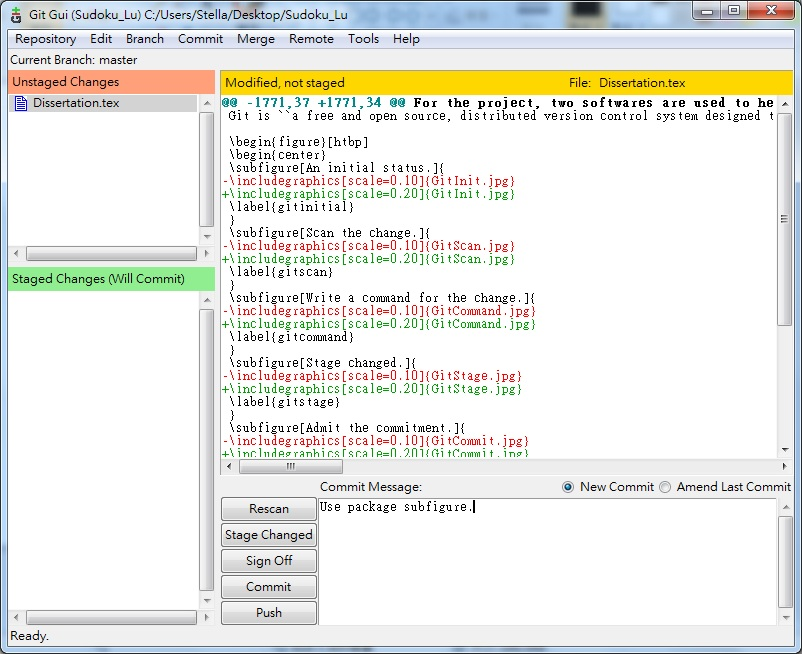
\includegraphics[scale=0.28]{GitScan.jpg}
\label{fig:gitscan}}
\subfigure[Write a command for the change.]{
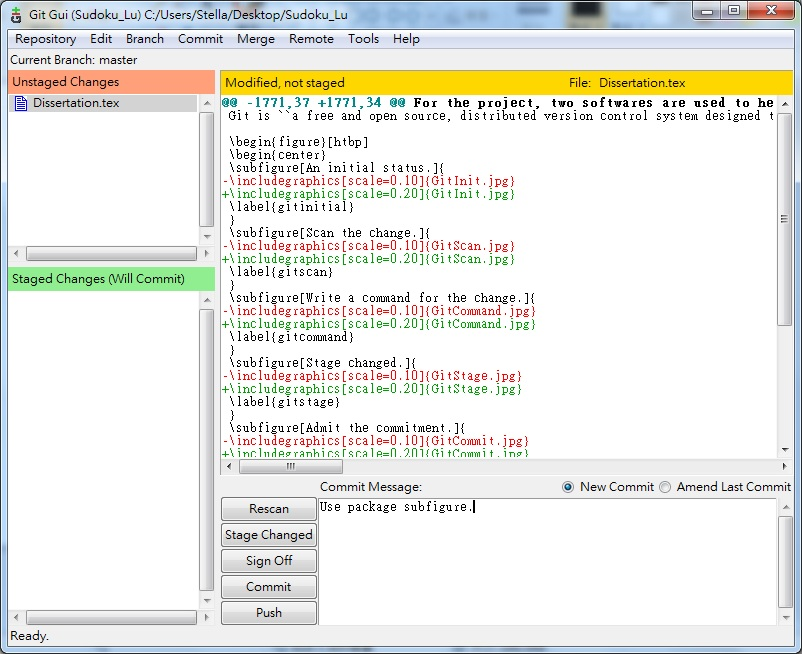
\includegraphics[scale=0.28]{GitCommand.jpg}
\label{fig:gitcommand}}
\subfigure[Stage changed.]{
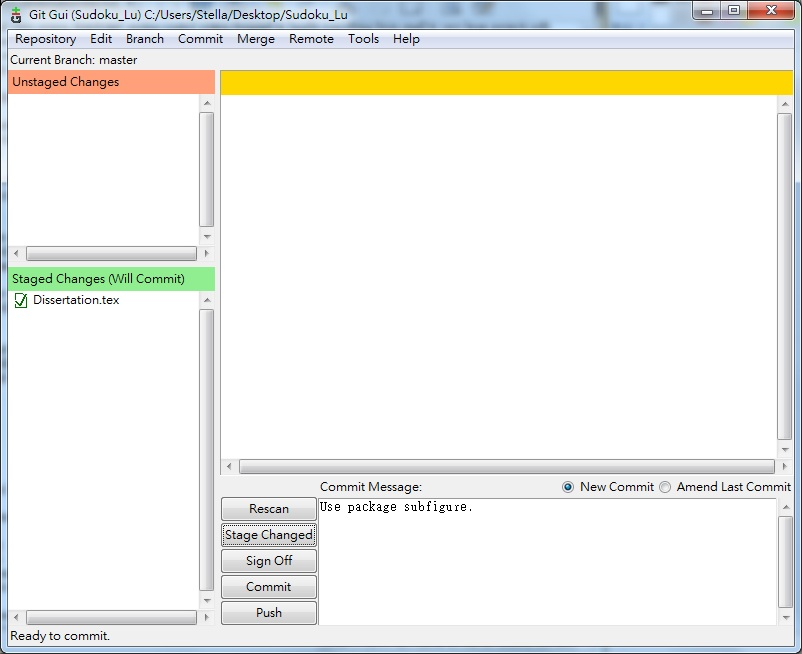
\includegraphics[scale=0.28]{GitStage.jpg}
\label{fig:gitstage}}
\subfigure[Admit the commitment.]{
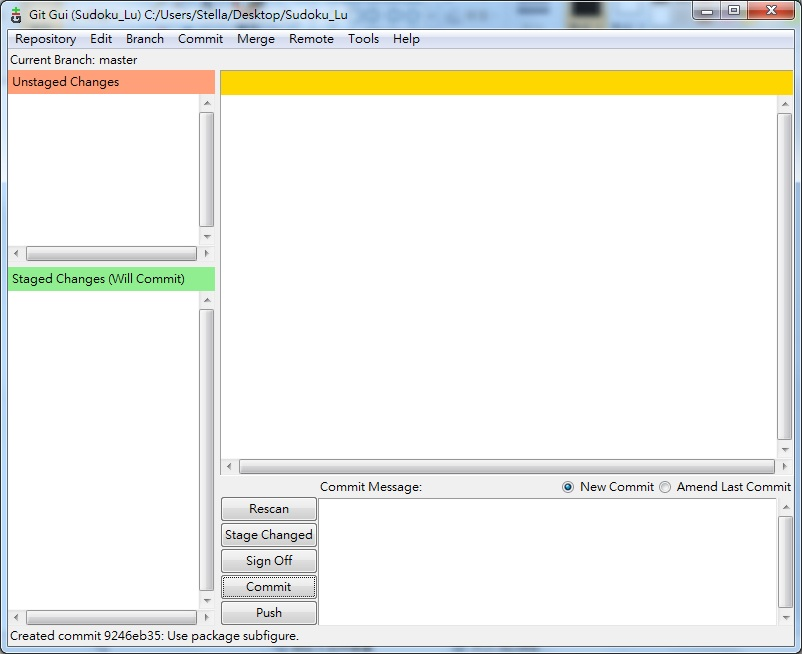
\includegraphics[scale=0.28]{GitCommit.jpg}
\label{fig:gitcommit}}
\end{center}
\end{figure}



\section{LaTex}
\label{sec:latex}
LaTeX is a document preparation system for high-quality typesetting. It is most often used for medium-to-large technical or scientific documents but it can be used for almost any form of publishing.

\subsection{Package usage}
\label{sec:packageusage}
\textbf{Usepackage} Use a package or a style.
\begin{verbatim}
\usepackage{package_name}
\end{verbatim}

\subsection{Sectioning}
\label{sec:sectioning}
Latex allows user to structure their document in order by chapters, sections, subsections and paragraphs. Here, we use chapters, sections, and subsections only by the commands:

\begin{verbatim}
\chapter{chapter}
\section{section}
\subsetion{subsection}
\end{verbatim}

\subsection{Figures, tables and pictures}
\label{sec:figurestablesandpictures}
\textbf{Pictures} Insert a picture into the document and specify the width.
\begin{verbatim}
\begin{figure}[location]
\includegraphics[width]{source}
\end{figure}
\end{verbatim}

\textbf{Sudoku} Which is import from a package ``Sudoku'' to generate a Sudoku matrix.
\begin{verbatim}
\begin{figure}[location]
\begin{sudoku}
\end{sudoku}
\end{figure}
\end{verbatim}

\subsection{Referencing and bibliography}
\label{sec:referencingandbibliography}

\textbf{Label} Give a mark to an object you want to reference.\\
\textbf{Ref} Reference the object you have previously marked.
\begin{verbatim}
\label{marker}
\ref{marker}
\end{verbatim}

\textbf{Footnote} providing extra information to the reader.
\begin{verbatim}
\footnote[num]{text}
\end{verbatim}

\textbf{Cite} Cite one of the references on your bibliography list. This can be done and providing the corresponding keyword that has already been assigned to an item in the bib file[\cite{Lamport1994LATEX}, 156].
\begin{verbatim}
\cite[page number]{item}
\end{verbatim}

A bib file provides many different entries to list referencing sources which is used to support the report. But in this report, we have only three type of entries used in the bib file, they are: three different source, book, journal, and website.

\textbf{Book} A book source which with an explicit publisher. Required fields: author, title, publisher, year. Optional fields: volume or number, series, address, edition, month, note. Here is an example:
\begin{verbatim}
@Book{Berthier2007Sudoku,
  author =	{Denis Berthier},
  title =	{The Hidden Logic of Sudoku},
  publisher =	{Lulu.com},
  year =	{2007},
  edition =	{Second},
  note =	{ISBN 978-1-84799-214-7},
}
\end{verbatim}
\textbf{Article} A article from a journal or magazine. Required fields: author, title, journal, year. Optional fields: volume, number, pages, month, note. Here is an example:
\begin{verbatim}
@Article{FelgenhauerJarvis2006SudokuI,
  author = 	 {Bertam Felgenhauer and Frazer Jarvis},
  title = 	 {Mathematics of {S}udoku {I}},
  journal = 	 {Mathematical Spectrum},
  year = 	 {2006},
  volume =	 {39},
  number =	 {1},
  pages =	 {15-22},
  month =	 {September},
  note =	 {Available at \url{http://www.afjarvis.staff.shef.ac.uk/maths/}}
}
\end{verbatim}
\textbf{Misc} Use this type when nothing else fits. Required fields: none. Optional fields: author, title, howpublished, month, year, note.Here is an example:
To add a website source to bibliographies:
\begin{verbatim}
@Misc{website:LeonhardEuler,
   author =	{Wikipedia},
   title =	{{Leonhard Euler --- Wikipedia{,} The Free Encyclopedia}},
   year =	{2011},
   url =		{http://en.wikipedia.org/wiki/Leonhard\_Euler},
   annote =	{Online; accessed 16-September-2011}
 }
\end{verbatim}


\chapter{Conclusion}
\label{cha:Conclusion}
The Sudoku puzzle might be solved by only one technique in some simple case Nevertheless, usually two or more are commonly needed in dealing general problem such like using both naked single and hidden single. The number of techniques used will increase according to the difficulty of the puzzle. The harder problem needs more complex technique to support it.
These special approaches for solving puzzle are simple and in fact popularly used in general problem solving. They are efficient to support player to eliminate the impossibilities in the cells, and leave the rest possibilities to get to the final solution.


\bibliographystyle{plain}

\bibliography{Sudoku}

\end{document}
